% Options for packages loaded elsewhere
\PassOptionsToPackage{unicode}{hyperref}
\PassOptionsToPackage{hyphens}{url}
\PassOptionsToPackage{dvipsnames,svgnames,x11names}{xcolor}
%
\documentclass[
  letterpaper,
  DIV=11,
  numbers=noendperiod]{scrartcl}

\usepackage{amsmath,amssymb}
\usepackage{iftex}
\ifPDFTeX
  \usepackage[T1]{fontenc}
  \usepackage[utf8]{inputenc}
  \usepackage{textcomp} % provide euro and other symbols
\else % if luatex or xetex
  \usepackage{unicode-math}
  \defaultfontfeatures{Scale=MatchLowercase}
  \defaultfontfeatures[\rmfamily]{Ligatures=TeX,Scale=1}
\fi
\usepackage{lmodern}
\ifPDFTeX\else  
    % xetex/luatex font selection
\fi
% Use upquote if available, for straight quotes in verbatim environments
\IfFileExists{upquote.sty}{\usepackage{upquote}}{}
\IfFileExists{microtype.sty}{% use microtype if available
  \usepackage[]{microtype}
  \UseMicrotypeSet[protrusion]{basicmath} % disable protrusion for tt fonts
}{}
\makeatletter
\@ifundefined{KOMAClassName}{% if non-KOMA class
  \IfFileExists{parskip.sty}{%
    \usepackage{parskip}
  }{% else
    \setlength{\parindent}{0pt}
    \setlength{\parskip}{6pt plus 2pt minus 1pt}}
}{% if KOMA class
  \KOMAoptions{parskip=half}}
\makeatother
\usepackage{xcolor}
\usepackage{soul}
\setlength{\emergencystretch}{3em} % prevent overfull lines
\setcounter{secnumdepth}{-\maxdimen} % remove section numbering
% Make \paragraph and \subparagraph free-standing
\ifx\paragraph\undefined\else
  \let\oldparagraph\paragraph
  \renewcommand{\paragraph}[1]{\oldparagraph{#1}\mbox{}}
\fi
\ifx\subparagraph\undefined\else
  \let\oldsubparagraph\subparagraph
  \renewcommand{\subparagraph}[1]{\oldsubparagraph{#1}\mbox{}}
\fi

\usepackage{color}
\usepackage{fancyvrb}
\newcommand{\VerbBar}{|}
\newcommand{\VERB}{\Verb[commandchars=\\\{\}]}
\DefineVerbatimEnvironment{Highlighting}{Verbatim}{commandchars=\\\{\}}
% Add ',fontsize=\small' for more characters per line
\usepackage{framed}
\definecolor{shadecolor}{RGB}{241,243,245}
\newenvironment{Shaded}{\begin{snugshade}}{\end{snugshade}}
\newcommand{\AlertTok}[1]{\textcolor[rgb]{0.68,0.00,0.00}{#1}}
\newcommand{\AnnotationTok}[1]{\textcolor[rgb]{0.37,0.37,0.37}{#1}}
\newcommand{\AttributeTok}[1]{\textcolor[rgb]{0.40,0.45,0.13}{#1}}
\newcommand{\BaseNTok}[1]{\textcolor[rgb]{0.68,0.00,0.00}{#1}}
\newcommand{\BuiltInTok}[1]{\textcolor[rgb]{0.00,0.23,0.31}{#1}}
\newcommand{\CharTok}[1]{\textcolor[rgb]{0.13,0.47,0.30}{#1}}
\newcommand{\CommentTok}[1]{\textcolor[rgb]{0.37,0.37,0.37}{#1}}
\newcommand{\CommentVarTok}[1]{\textcolor[rgb]{0.37,0.37,0.37}{\textit{#1}}}
\newcommand{\ConstantTok}[1]{\textcolor[rgb]{0.56,0.35,0.01}{#1}}
\newcommand{\ControlFlowTok}[1]{\textcolor[rgb]{0.00,0.23,0.31}{#1}}
\newcommand{\DataTypeTok}[1]{\textcolor[rgb]{0.68,0.00,0.00}{#1}}
\newcommand{\DecValTok}[1]{\textcolor[rgb]{0.68,0.00,0.00}{#1}}
\newcommand{\DocumentationTok}[1]{\textcolor[rgb]{0.37,0.37,0.37}{\textit{#1}}}
\newcommand{\ErrorTok}[1]{\textcolor[rgb]{0.68,0.00,0.00}{#1}}
\newcommand{\ExtensionTok}[1]{\textcolor[rgb]{0.00,0.23,0.31}{#1}}
\newcommand{\FloatTok}[1]{\textcolor[rgb]{0.68,0.00,0.00}{#1}}
\newcommand{\FunctionTok}[1]{\textcolor[rgb]{0.28,0.35,0.67}{#1}}
\newcommand{\ImportTok}[1]{\textcolor[rgb]{0.00,0.46,0.62}{#1}}
\newcommand{\InformationTok}[1]{\textcolor[rgb]{0.37,0.37,0.37}{#1}}
\newcommand{\KeywordTok}[1]{\textcolor[rgb]{0.00,0.23,0.31}{#1}}
\newcommand{\NormalTok}[1]{\textcolor[rgb]{0.00,0.23,0.31}{#1}}
\newcommand{\OperatorTok}[1]{\textcolor[rgb]{0.37,0.37,0.37}{#1}}
\newcommand{\OtherTok}[1]{\textcolor[rgb]{0.00,0.23,0.31}{#1}}
\newcommand{\PreprocessorTok}[1]{\textcolor[rgb]{0.68,0.00,0.00}{#1}}
\newcommand{\RegionMarkerTok}[1]{\textcolor[rgb]{0.00,0.23,0.31}{#1}}
\newcommand{\SpecialCharTok}[1]{\textcolor[rgb]{0.37,0.37,0.37}{#1}}
\newcommand{\SpecialStringTok}[1]{\textcolor[rgb]{0.13,0.47,0.30}{#1}}
\newcommand{\StringTok}[1]{\textcolor[rgb]{0.13,0.47,0.30}{#1}}
\newcommand{\VariableTok}[1]{\textcolor[rgb]{0.07,0.07,0.07}{#1}}
\newcommand{\VerbatimStringTok}[1]{\textcolor[rgb]{0.13,0.47,0.30}{#1}}
\newcommand{\WarningTok}[1]{\textcolor[rgb]{0.37,0.37,0.37}{\textit{#1}}}

\providecommand{\tightlist}{%
  \setlength{\itemsep}{0pt}\setlength{\parskip}{0pt}}\usepackage{longtable,booktabs,array}
\usepackage{calc} % for calculating minipage widths
% Correct order of tables after \paragraph or \subparagraph
\usepackage{etoolbox}
\makeatletter
\patchcmd\longtable{\par}{\if@noskipsec\mbox{}\fi\par}{}{}
\makeatother
% Allow footnotes in longtable head/foot
\IfFileExists{footnotehyper.sty}{\usepackage{footnotehyper}}{\usepackage{footnote}}
\makesavenoteenv{longtable}
\usepackage{graphicx}
\makeatletter
\def\maxwidth{\ifdim\Gin@nat@width>\linewidth\linewidth\else\Gin@nat@width\fi}
\def\maxheight{\ifdim\Gin@nat@height>\textheight\textheight\else\Gin@nat@height\fi}
\makeatother
% Scale images if necessary, so that they will not overflow the page
% margins by default, and it is still possible to overwrite the defaults
% using explicit options in \includegraphics[width, height, ...]{}
\setkeys{Gin}{width=\maxwidth,height=\maxheight,keepaspectratio}
% Set default figure placement to htbp
\makeatletter
\def\fps@figure{htbp}
\makeatother

\usepackage{booktabs}
\usepackage{caption}
\usepackage{longtable}
\usepackage{colortbl}
\usepackage{array}
\KOMAoption{captions}{tableheading}
\makeatletter
\makeatother
\makeatletter
\makeatother
\makeatletter
\@ifpackageloaded{caption}{}{\usepackage{caption}}
\AtBeginDocument{%
\ifdefined\contentsname
  \renewcommand*\contentsname{Table of contents}
\else
  \newcommand\contentsname{Table of contents}
\fi
\ifdefined\listfigurename
  \renewcommand*\listfigurename{List of Figures}
\else
  \newcommand\listfigurename{List of Figures}
\fi
\ifdefined\listtablename
  \renewcommand*\listtablename{List of Tables}
\else
  \newcommand\listtablename{List of Tables}
\fi
\ifdefined\figurename
  \renewcommand*\figurename{Figure}
\else
  \newcommand\figurename{Figure}
\fi
\ifdefined\tablename
  \renewcommand*\tablename{Table}
\else
  \newcommand\tablename{Table}
\fi
}
\@ifpackageloaded{float}{}{\usepackage{float}}
\floatstyle{ruled}
\@ifundefined{c@chapter}{\newfloat{codelisting}{h}{lop}}{\newfloat{codelisting}{h}{lop}[chapter]}
\floatname{codelisting}{Listing}
\newcommand*\listoflistings{\listof{codelisting}{List of Listings}}
\makeatother
\makeatletter
\@ifpackageloaded{caption}{}{\usepackage{caption}}
\@ifpackageloaded{subcaption}{}{\usepackage{subcaption}}
\makeatother
\makeatletter
\@ifpackageloaded{tcolorbox}{}{\usepackage[skins,breakable]{tcolorbox}}
\makeatother
\makeatletter
\@ifundefined{shadecolor}{\definecolor{shadecolor}{rgb}{.97, .97, .97}}
\makeatother
\makeatletter
\makeatother
\makeatletter
\makeatother
\ifLuaTeX
  \usepackage{selnolig}  % disable illegal ligatures
\fi
\IfFileExists{bookmark.sty}{\usepackage{bookmark}}{\usepackage{hyperref}}
\IfFileExists{xurl.sty}{\usepackage{xurl}}{} % add URL line breaks if available
\urlstyle{same} % disable monospaced font for URLs
\hypersetup{
  pdftitle={Machine Learning Project 2024},
  pdfauthor={Lucas Jakin; Saša Nanut; Luca Marega},
  colorlinks=true,
  linkcolor={blue},
  filecolor={Maroon},
  citecolor={Blue},
  urlcolor={Blue},
  pdfcreator={LaTeX via pandoc}}

\title{Machine Learning Project 2024}
\author{Lucas Jakin \and Saša Nanut \and Luca Marega}
\date{2024-06-04}

\begin{document}
\maketitle
\ifdefined\Shaded\renewenvironment{Shaded}{\begin{tcolorbox}[breakable, borderline west={3pt}{0pt}{shadecolor}, sharp corners, interior hidden, frame hidden, enhanced, boxrule=0pt]}{\end{tcolorbox}}\fi

\renewcommand*\contentsname{Table of contents}
{
\hypersetup{linkcolor=}
\setcounter{tocdepth}{3}
\tableofcontents
}
\hypertarget{predicting-next-day-rain-in-australia}{%
\section{Predicting next-day rain in
Australia}\label{predicting-next-day-rain-in-australia}}

\hypertarget{introduction}{%
\paragraph{Introduction}\label{introduction}}

As a group we decided to take on the \textbf{first project type}. The
project focuses on utilizing DM \& ML algorithms to address a specific
problem chosen from Kaggle.The Goal of the project is to address the
classification problem by utilizing more than one classification
algorithm, in order to do a systematic experimentation with different
algorithms to identify in what they differ and which one is the most
effective one for the chosen dataset. We will consider different
classification algorithms and make the comparison between three of them,
more precisely \emph{Artificial Neural Networks}, \emph{CatBoost} and
\emph{Logistic Regression}.\\

We will divide the work as the following: as a group we will perform a
brief analysis of the dataset and make some cleaning of it if needed.
Afterwards, each one of us will implement one of the previously
mentioned algorithms and then we will compare and interpret the results

\hypertarget{about-the-dataset}{%
\subsection{About the dataset}\label{about-the-dataset}}

The dataset found in
\href{https://www.kaggle.com/datasets/jsphyg/weather-dataset-rattle-package/code}{Kaggle}
consists of about 10 years of daily weather observations from numerous
locations across Australia.\\

The problem that is required to be solved from this dataset represents a
classification problem, in this case a \textbf{binary classification}
problem. The objective is to predict whether it will rain tomorrow or
not with high accuracy. The dataframe contains 145460 observations
(rows) and 23 attributes. The observations are weather conditions of
days of a specific region including: date, location, minimum and maximum
temperature, rain fall, humidity and so on.\\

The most important feature of the dataset is the last column
\textbf{``RainTomorrow''}, which is the target variable for our ML
models that we want to predict.

It has two values:

\begin{itemize}
\item
  Yes --\textgreater{} It will rain tomorrow
\item
  No --\textgreater{} It will not rain tomorrow.
\end{itemize}

\hypertarget{exploratory-data-analysis}{%
\subsection{Exploratory Data Analysis}\label{exploratory-data-analysis}}

\begin{Shaded}
\begin{Highlighting}[]
\FunctionTok{library}\NormalTok{(tidyverse)}
\FunctionTok{library}\NormalTok{(dplyr)}
\FunctionTok{library}\NormalTok{(skimr)}
\FunctionTok{library}\NormalTok{(ggcorrplot)}
\FunctionTok{library}\NormalTok{(gt)}
\FunctionTok{library}\NormalTok{(ggplot2)}

\CommentTok{\#use\_python("C:\textbackslash{}\textbackslash{}Python312\textbackslash{}python.exe", required = T)}
\NormalTok{weatherAus }\OtherTok{\textless{}{-}} \FunctionTok{read.csv}\NormalTok{(}\StringTok{"weatherAUS.csv"}\NormalTok{, }\AttributeTok{header =}\NormalTok{ T)}
\end{Highlighting}
\end{Shaded}

Setting up python into Rstudio:

\begin{Shaded}
\begin{Highlighting}[]
\CommentTok{\# SETTING UP PYTHON ON RSTUDIO}
\FunctionTok{library}\NormalTok{(reticulate)}

\FunctionTok{virtualenv\_create}\NormalTok{(}\StringTok{"my{-}python"}\NormalTok{, }\AttributeTok{python\_version =} \StringTok{"3.12"}\NormalTok{)}
\FunctionTok{use\_virtualenv}\NormalTok{(}\StringTok{"my{-}python"}\NormalTok{, }\AttributeTok{required =} \ConstantTok{TRUE}\NormalTok{)}

\CommentTok{\#virtualenv\_install(envname = "my{-}python", "matplotlib",ignore\_installed = FALSE, pip\_options = character())}

\CommentTok{\#virtualenv\_install(envname = "my{-}python", "catboost",ignore\_installed = FALSE, pip\_options = character())}

\CommentTok{\#virtualenv\_install(envname = "my{-}python", "numpy",ignore\_installed = FALSE, pip\_options = character())}

\CommentTok{\#virtualenv\_install(envname = "my{-}python", "pandas",ignore\_installed = FALSE, pip\_options = character())}

\CommentTok{\#virtualenv\_install(envname = "my{-}python", "seaborn",ignore\_installed = FALSE, pip\_options = character())}

\CommentTok{\#virtualenv\_install(envname = "my{-}python", "scikit{-}learn",ignore\_installed = FALSE, pip\_options = character())}

\CommentTok{\#virtualenv\_install(envname = "my{-}python", "tensorflow",ignore\_installed = FALSE, pip\_options = character())}
\end{Highlighting}
\end{Shaded}

\begin{center}\rule{0.5\linewidth}{0.5pt}\end{center}

As we start, we first load the weather data and look at the first rows
to identify the features:

\begin{Shaded}
\begin{Highlighting}[]
\FunctionTok{head}\NormalTok{(weatherAus) }\SpecialCharTok{\%\textgreater{}\%} \FunctionTok{gt}\NormalTok{()}
\end{Highlighting}
\end{Shaded}

\begin{longtable*}{rlrrrrrlrllrrrrrrrrrrll}
\toprule
Date & Location & MinTemp & MaxTemp & Rainfall & Evaporation & Sunshine & WindGustDir & WindGustSpeed & WindDir9am & WindDir3pm & WindSpeed9am & WindSpeed3pm & Humidity9am & Humidity3pm & Pressure9am & Pressure3pm & Cloud9am & Cloud3pm & Temp9am & Temp3pm & RainToday & RainTomorrow \\ 
\midrule\addlinespace[2.5pt]
2008-12-01 & Albury & 13.4 & 22.9 & 0.6 & NA & NA & W & 44 & W & WNW & 20 & 24 & 71 & 22 & 1007.7 & 1007.1 & 8 & NA & 16.9 & 21.8 & No & No \\ 
2008-12-02 & Albury & 7.4 & 25.1 & 0.0 & NA & NA & WNW & 44 & NNW & WSW & 4 & 22 & 44 & 25 & 1010.6 & 1007.8 & NA & NA & 17.2 & 24.3 & No & No \\ 
2008-12-03 & Albury & 12.9 & 25.7 & 0.0 & NA & NA & WSW & 46 & W & WSW & 19 & 26 & 38 & 30 & 1007.6 & 1008.7 & NA & 2 & 21.0 & 23.2 & No & No \\ 
2008-12-04 & Albury & 9.2 & 28.0 & 0.0 & NA & NA & NE & 24 & SE & E & 11 & 9 & 45 & 16 & 1017.6 & 1012.8 & NA & NA & 18.1 & 26.5 & No & No \\ 
2008-12-05 & Albury & 17.5 & 32.3 & 1.0 & NA & NA & W & 41 & ENE & NW & 7 & 20 & 82 & 33 & 1010.8 & 1006.0 & 7 & 8 & 17.8 & 29.7 & No & No \\ 
2008-12-06 & Albury & 14.6 & 29.7 & 0.2 & NA & NA & WNW & 56 & W & W & 19 & 24 & 55 & 23 & 1009.2 & 1005.4 & NA & NA & 20.6 & 28.9 & No & No \\ 
\bottomrule
\end{longtable*}

\hfill\break
In the next step we check out the summary statistics of the dataset and
identify the numerical and categorical attributes:

\begin{Shaded}
\begin{Highlighting}[]
\FunctionTok{skim}\NormalTok{(weatherAus)}
\end{Highlighting}
\end{Shaded}

\begin{longtable}[]{@{}ll@{}}
\caption{Data summary}\tabularnewline
\toprule\noalign{}
\endfirsthead
\endhead
\bottomrule\noalign{}
\endlastfoot
Name & weatherAus \\
Number of rows & 145460 \\
Number of columns & 23 \\
\_\_\_\_\_\_\_\_\_\_\_\_\_\_\_\_\_\_\_\_\_\_\_ & \\
Column type frequency: & \\
character & 7 \\
numeric & 16 \\
\_\_\_\_\_\_\_\_\_\_\_\_\_\_\_\_\_\_\_\_\_\_\_\_ & \\
Group variables & None \\
\end{longtable}

\textbf{Variable type: character}

\begin{longtable}[]{@{}
  >{\raggedright\arraybackslash}p{(\columnwidth - 14\tabcolsep) * \real{0.1944}}
  >{\raggedleft\arraybackslash}p{(\columnwidth - 14\tabcolsep) * \real{0.1389}}
  >{\raggedleft\arraybackslash}p{(\columnwidth - 14\tabcolsep) * \real{0.1944}}
  >{\raggedleft\arraybackslash}p{(\columnwidth - 14\tabcolsep) * \real{0.0556}}
  >{\raggedleft\arraybackslash}p{(\columnwidth - 14\tabcolsep) * \real{0.0556}}
  >{\raggedleft\arraybackslash}p{(\columnwidth - 14\tabcolsep) * \real{0.0833}}
  >{\raggedleft\arraybackslash}p{(\columnwidth - 14\tabcolsep) * \real{0.1250}}
  >{\raggedleft\arraybackslash}p{(\columnwidth - 14\tabcolsep) * \real{0.1528}}@{}}
\toprule\noalign{}
\begin{minipage}[b]{\linewidth}\raggedright
skim\_variable
\end{minipage} & \begin{minipage}[b]{\linewidth}\raggedleft
n\_missing
\end{minipage} & \begin{minipage}[b]{\linewidth}\raggedleft
complete\_rate
\end{minipage} & \begin{minipage}[b]{\linewidth}\raggedleft
min
\end{minipage} & \begin{minipage}[b]{\linewidth}\raggedleft
max
\end{minipage} & \begin{minipage}[b]{\linewidth}\raggedleft
empty
\end{minipage} & \begin{minipage}[b]{\linewidth}\raggedleft
n\_unique
\end{minipage} & \begin{minipage}[b]{\linewidth}\raggedleft
whitespace
\end{minipage} \\
\midrule\noalign{}
\endhead
\bottomrule\noalign{}
\endlastfoot
Date & 0 & 1.00 & 10 & 10 & 0 & 3436 & 0 \\
Location & 0 & 1.00 & 4 & 16 & 0 & 49 & 0 \\
WindGustDir & 10326 & 0.93 & 1 & 3 & 0 & 16 & 0 \\
WindDir9am & 10566 & 0.93 & 1 & 3 & 0 & 16 & 0 \\
WindDir3pm & 4228 & 0.97 & 1 & 3 & 0 & 16 & 0 \\
RainToday & 3261 & 0.98 & 2 & 3 & 0 & 2 & 0 \\
RainTomorrow & 3267 & 0.98 & 2 & 3 & 0 & 2 & 0 \\
\end{longtable}

\textbf{Variable type: numeric}

\begin{longtable}[]{@{}
  >{\raggedright\arraybackslash}p{(\columnwidth - 20\tabcolsep) * \real{0.1522}}
  >{\raggedleft\arraybackslash}p{(\columnwidth - 20\tabcolsep) * \real{0.1087}}
  >{\raggedleft\arraybackslash}p{(\columnwidth - 20\tabcolsep) * \real{0.1522}}
  >{\raggedleft\arraybackslash}p{(\columnwidth - 20\tabcolsep) * \real{0.0870}}
  >{\raggedleft\arraybackslash}p{(\columnwidth - 20\tabcolsep) * \real{0.0652}}
  >{\raggedleft\arraybackslash}p{(\columnwidth - 20\tabcolsep) * \real{0.0652}}
  >{\raggedleft\arraybackslash}p{(\columnwidth - 20\tabcolsep) * \real{0.0761}}
  >{\raggedleft\arraybackslash}p{(\columnwidth - 20\tabcolsep) * \real{0.0761}}
  >{\raggedleft\arraybackslash}p{(\columnwidth - 20\tabcolsep) * \real{0.0761}}
  >{\raggedleft\arraybackslash}p{(\columnwidth - 20\tabcolsep) * \real{0.0761}}
  >{\raggedright\arraybackslash}p{(\columnwidth - 20\tabcolsep) * \real{0.0652}}@{}}
\toprule\noalign{}
\begin{minipage}[b]{\linewidth}\raggedright
skim\_variable
\end{minipage} & \begin{minipage}[b]{\linewidth}\raggedleft
n\_missing
\end{minipage} & \begin{minipage}[b]{\linewidth}\raggedleft
complete\_rate
\end{minipage} & \begin{minipage}[b]{\linewidth}\raggedleft
mean
\end{minipage} & \begin{minipage}[b]{\linewidth}\raggedleft
sd
\end{minipage} & \begin{minipage}[b]{\linewidth}\raggedleft
p0
\end{minipage} & \begin{minipage}[b]{\linewidth}\raggedleft
p25
\end{minipage} & \begin{minipage}[b]{\linewidth}\raggedleft
p50
\end{minipage} & \begin{minipage}[b]{\linewidth}\raggedleft
p75
\end{minipage} & \begin{minipage}[b]{\linewidth}\raggedleft
p100
\end{minipage} & \begin{minipage}[b]{\linewidth}\raggedright
hist
\end{minipage} \\
\midrule\noalign{}
\endhead
\bottomrule\noalign{}
\endlastfoot
MinTemp & 1485 & 0.99 & 12.19 & 6.40 & -8.5 & 7.6 & 12.0 & 16.9 & 33.9 &
▁▅▇▅▁ \\
MaxTemp & 1261 & 0.99 & 23.22 & 7.12 & -4.8 & 17.9 & 22.6 & 28.2 & 48.1
& ▁▂▇▅▁ \\
Rainfall & 3261 & 0.98 & 2.36 & 8.48 & 0.0 & 0.0 & 0.0 & 0.8 & 371.0 &
▇▁▁▁▁ \\
Evaporation & 62790 & 0.57 & 5.47 & 4.19 & 0.0 & 2.6 & 4.8 & 7.4 & 145.0
& ▇▁▁▁▁ \\
Sunshine & 69835 & 0.52 & 7.61 & 3.79 & 0.0 & 4.8 & 8.4 & 10.6 & 14.5 &
▃▃▅▇▃ \\
WindGustSpeed & 10263 & 0.93 & 40.04 & 13.61 & 6.0 & 31.0 & 39.0 & 48.0
& 135.0 & ▅▇▁▁▁ \\
WindSpeed9am & 1767 & 0.99 & 14.04 & 8.92 & 0.0 & 7.0 & 13.0 & 19.0 &
130.0 & ▇▁▁▁▁ \\
WindSpeed3pm & 3062 & 0.98 & 18.66 & 8.81 & 0.0 & 13.0 & 19.0 & 24.0 &
87.0 & ▇▇▁▁▁ \\
Humidity9am & 2654 & 0.98 & 68.88 & 19.03 & 0.0 & 57.0 & 70.0 & 83.0 &
100.0 & ▁▁▅▇▆ \\
Humidity3pm & 4507 & 0.97 & 51.54 & 20.80 & 0.0 & 37.0 & 52.0 & 66.0 &
100.0 & ▂▅▇▆▂ \\
Pressure9am & 15065 & 0.90 & 1017.65 & 7.11 & 980.5 & 1012.9 & 1017.6 &
1022.4 & 1041.0 & ▁▁▇▇▁ \\
Pressure3pm & 15028 & 0.90 & 1015.26 & 7.04 & 977.1 & 1010.4 & 1015.2 &
1020.0 & 1039.6 & ▁▁▇▇▁ \\
Cloud9am & 55888 & 0.62 & 4.45 & 2.89 & 0.0 & 1.0 & 5.0 & 7.0 & 9.0 &
▇▃▃▇▅ \\
Cloud3pm & 59358 & 0.59 & 4.51 & 2.72 & 0.0 & 2.0 & 5.0 & 7.0 & 9.0 &
▆▅▃▇▃ \\
Temp9am & 1767 & 0.99 & 16.99 & 6.49 & -7.2 & 12.3 & 16.7 & 21.6 & 40.2
& ▁▃▇▃▁ \\
Temp3pm & 3609 & 0.98 & 21.68 & 6.94 & -5.4 & 16.6 & 21.1 & 26.4 & 46.7
& ▁▃▇▃▁ \\
\end{longtable}

As we can see from the figure above, there are 7 \textbf{categorical}
attributes and 16 \textbf{numerical} attributes.\\
Before taking a deeper look on all other attributes, we first did a
brief exploration of the target variable:

\begin{itemize}
\tightlist
\item
  \textbf{MISSING VALUES}
\end{itemize}

\begin{Shaded}
\begin{Highlighting}[]
\NormalTok{missingValues }\OtherTok{\textless{}{-}} \FunctionTok{sum}\NormalTok{(}\FunctionTok{is.na}\NormalTok{(weatherAus}\SpecialCharTok{$}\NormalTok{RainTomorrow))}
\NormalTok{missingValues}
\end{Highlighting}
\end{Shaded}

\begin{verbatim}
[1] 3267
\end{verbatim}

\begin{itemize}
\tightlist
\item
  \textbf{FREQUENCY DISTRIBUTION OF VALUES}
\end{itemize}

\begin{Shaded}
\begin{Highlighting}[]
\NormalTok{  weatherAus }\SpecialCharTok{\%\textgreater{}\%} \FunctionTok{select}\NormalTok{(RainTomorrow) }\SpecialCharTok{\%\textgreater{}\%}
  \FunctionTok{count}\NormalTok{(RainTomorrow) }\SpecialCharTok{\%\textgreater{}\%} \FunctionTok{drop\_na}\NormalTok{() }\SpecialCharTok{\%\textgreater{}\%}
  \FunctionTok{ggplot}\NormalTok{(., }\FunctionTok{aes}\NormalTok{(RainTomorrow, n, }\AttributeTok{fill=}\NormalTok{RainTomorrow)) }\SpecialCharTok{+}
  \FunctionTok{geom\_col}\NormalTok{(}\AttributeTok{width =} \FloatTok{0.5}\NormalTok{)}\SpecialCharTok{+}
  \FunctionTok{labs}\NormalTok{(}\AttributeTok{x =} \StringTok{"RainTomorrow"}\NormalTok{, }\AttributeTok{y =} \StringTok{"Count"}\NormalTok{)}\SpecialCharTok{+}
  \FunctionTok{theme\_minimal}\NormalTok{()}
\end{Highlighting}
\end{Shaded}

\begin{figure}[H]

{\centering 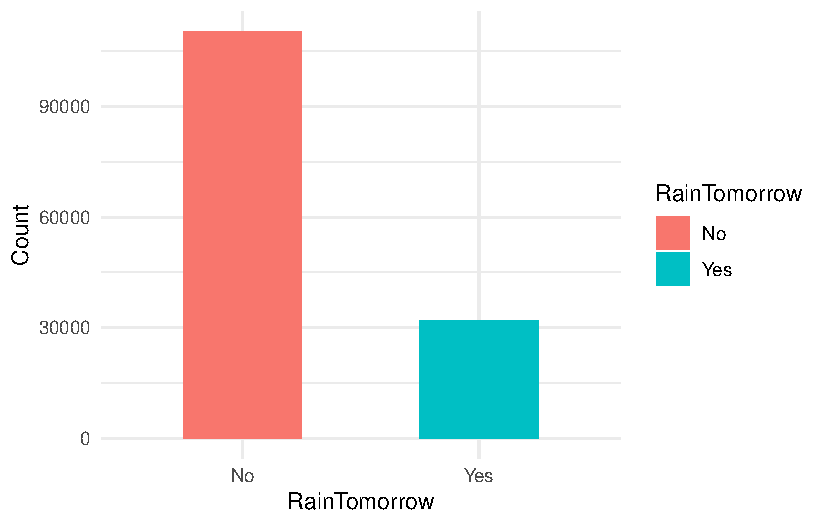
\includegraphics{RainAus_EDA_files/figure-pdf/unnamed-chunk-6-1.pdf}

}

\end{figure}

\begin{itemize}
\tightlist
\item
  \textbf{RATIO OF FREQUENCY DISTRIBUTION}
\end{itemize}

\begin{Shaded}
\begin{Highlighting}[]
\NormalTok{  weatherAus }\SpecialCharTok{\%\textgreater{}\%} \FunctionTok{select}\NormalTok{(RainTomorrow) }\SpecialCharTok{\%\textgreater{}\%}
  \FunctionTok{count}\NormalTok{(RainTomorrow) }\SpecialCharTok{\%\textgreater{}\%} \FunctionTok{drop\_na}\NormalTok{() }\SpecialCharTok{\%\textgreater{}\%}
  \FunctionTok{ggplot}\NormalTok{(., }\FunctionTok{aes}\NormalTok{(}\AttributeTok{x=}\StringTok{""}\NormalTok{, n, }\AttributeTok{fill =}\NormalTok{ RainTomorrow)) }\SpecialCharTok{+}
  \FunctionTok{geom\_bar}\NormalTok{(}\AttributeTok{width =} \DecValTok{1}\NormalTok{, }\AttributeTok{size =} \DecValTok{1}\NormalTok{, }\AttributeTok{color =} \StringTok{"white"}\NormalTok{,}\AttributeTok{stat =} \StringTok{"identity"}\NormalTok{) }\SpecialCharTok{+} \FunctionTok{coord\_polar}\NormalTok{(}\StringTok{"y"}\NormalTok{, }\AttributeTok{start =} \DecValTok{0}\NormalTok{) }\SpecialCharTok{+}
  \FunctionTok{geom\_text}\NormalTok{(}\FunctionTok{aes}\NormalTok{(}\AttributeTok{label =} \FunctionTok{paste0}\NormalTok{(}\FunctionTok{round}\NormalTok{((n}\SpecialCharTok{/}\DecValTok{145460}\NormalTok{)}\SpecialCharTok{*}\DecValTok{100}\NormalTok{),}\StringTok{"\%"}\NormalTok{)),}
            \AttributeTok{position =} \FunctionTok{position\_stack}\NormalTok{(}\AttributeTok{vjust =} \FloatTok{0.5}\NormalTok{)) }\SpecialCharTok{+}
  \FunctionTok{theme\_classic}\NormalTok{() }\SpecialCharTok{+}
  \FunctionTok{labs}\NormalTok{(}\AttributeTok{x =} \ConstantTok{NULL}\NormalTok{, }\AttributeTok{y =} \ConstantTok{NULL}\NormalTok{) }\SpecialCharTok{+}
  \FunctionTok{theme}\NormalTok{(}\AttributeTok{axis.line =} \FunctionTok{element\_blank}\NormalTok{())}
\end{Highlighting}
\end{Shaded}

\begin{figure}[H]

{\centering 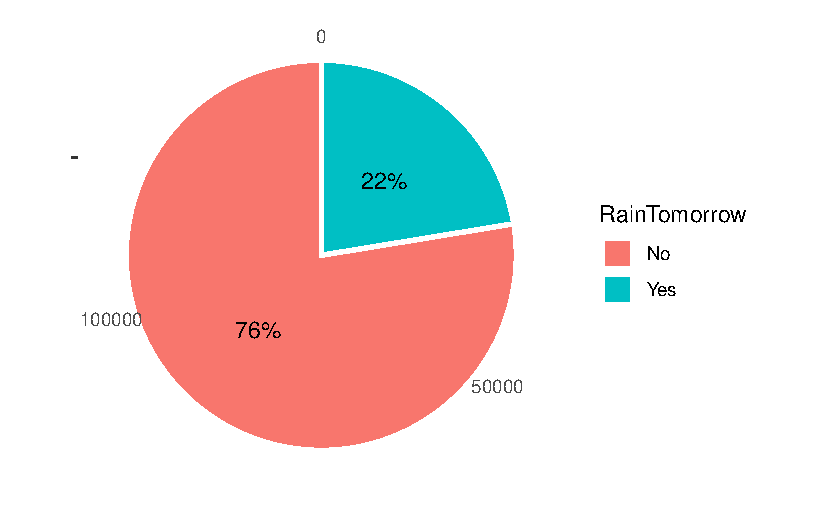
\includegraphics{RainAus_EDA_files/figure-pdf/unnamed-chunk-7-1.pdf}

}

\end{figure}

\hfill\break
From the plots drawn above, we can clearly see that RainTomorrow has 2
categories of values: \textbf{Yes} and \textbf{No}. There are far more
NEGATIVE values than POSITIVE.\emph{``No''} and \emph{``Yes''} appears
76\% of time and 22\% of time respectively after deleting all NA values
from the attribute.

\begin{Shaded}
\begin{Highlighting}[]
\NormalTok{  weatherAus }\SpecialCharTok{\%\textgreater{}\%} \FunctionTok{select}\NormalTok{(RainToday) }\SpecialCharTok{\%\textgreater{}\%}
  \FunctionTok{count}\NormalTok{(RainToday) }\SpecialCharTok{\%\textgreater{}\%} \FunctionTok{drop\_na}\NormalTok{() }\SpecialCharTok{\%\textgreater{}\%}
  \FunctionTok{ggplot}\NormalTok{(., }\FunctionTok{aes}\NormalTok{(}\AttributeTok{x=}\StringTok{""}\NormalTok{, n, }\AttributeTok{fill =}\NormalTok{ RainToday)) }\SpecialCharTok{+}
  \FunctionTok{geom\_bar}\NormalTok{(}\AttributeTok{width =} \DecValTok{1}\NormalTok{, }\AttributeTok{size =} \DecValTok{1}\NormalTok{, }\AttributeTok{color =} \StringTok{"white"}\NormalTok{,}\AttributeTok{stat =} \StringTok{"identity"}\NormalTok{) }\SpecialCharTok{+} \FunctionTok{coord\_polar}\NormalTok{(}\StringTok{"y"}\NormalTok{, }\AttributeTok{start =} \DecValTok{0}\NormalTok{) }\SpecialCharTok{+}
  \FunctionTok{geom\_text}\NormalTok{(}\FunctionTok{aes}\NormalTok{(}\AttributeTok{label =} \FunctionTok{paste0}\NormalTok{(}\FunctionTok{round}\NormalTok{((n}\SpecialCharTok{/}\DecValTok{145460}\NormalTok{)}\SpecialCharTok{*}\DecValTok{100}\NormalTok{),}\StringTok{"\%"}\NormalTok{)),}
            \AttributeTok{position =} \FunctionTok{position\_stack}\NormalTok{(}\AttributeTok{vjust =} \FloatTok{0.5}\NormalTok{)) }\SpecialCharTok{+}
  \FunctionTok{theme\_classic}\NormalTok{() }\SpecialCharTok{+}
  \FunctionTok{labs}\NormalTok{(}\AttributeTok{x =} \ConstantTok{NULL}\NormalTok{, }\AttributeTok{y =} \ConstantTok{NULL}\NormalTok{) }\SpecialCharTok{+}
  \FunctionTok{theme}\NormalTok{(}\AttributeTok{axis.line =} \FunctionTok{element\_blank}\NormalTok{())}
\end{Highlighting}
\end{Shaded}

\begin{figure}[H]

{\centering 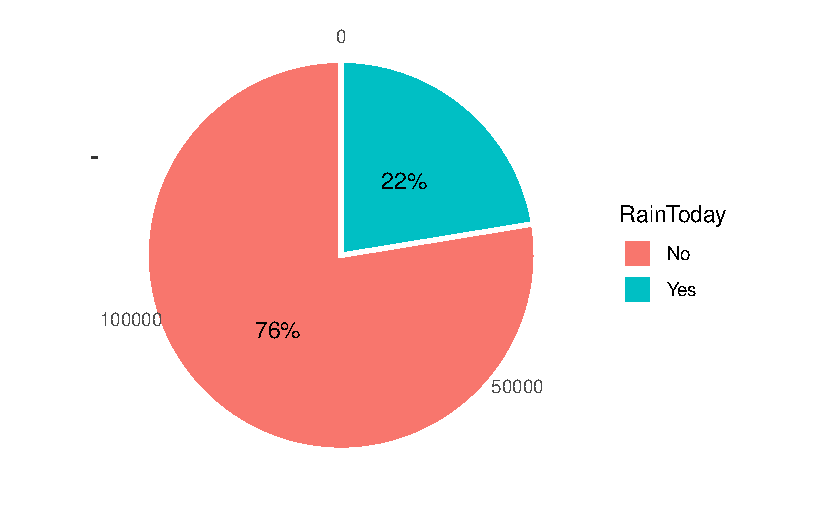
\includegraphics{RainAus_EDA_files/figure-pdf/unnamed-chunk-8-1.pdf}

}

\end{figure}

\hfill\break

The variable \textbf{RainToday} has a very similar value distribution as
the target variable. \ldots!!!!!!!!!!!!!!!!!!!!!

\begin{center}\rule{0.5\linewidth}{0.5pt}\end{center}

\hypertarget{categorical-values}{%
\subsubsection{Categorical values}\label{categorical-values}}

All together there are 6 categorical features + a Date column. In order
to make the information about the date more useful, we decided to
extract the year, the month and the day from the date into three
separate columns.\\
This is done here below:

\begin{Shaded}
\begin{Highlighting}[]
\NormalTok{weatherAusNew }\OtherTok{\textless{}{-}}\NormalTok{ weatherAus }\SpecialCharTok{\%\textgreater{}\%} \FunctionTok{mutate}\NormalTok{(}
  \AttributeTok{Year =} \FunctionTok{year}\NormalTok{(Date),}
  \AttributeTok{Month =} \FunctionTok{month}\NormalTok{(Date),}
  \AttributeTok{Day =} \FunctionTok{day}\NormalTok{(Date)}
\NormalTok{) }\SpecialCharTok{\%\textgreater{}\%} \FunctionTok{select}\NormalTok{(}\SpecialCharTok{{-}}\NormalTok{Date)}
\FunctionTok{as\_tibble}\NormalTok{(weatherAusNew)}
\end{Highlighting}
\end{Shaded}

\begin{verbatim}
# A tibble: 145,460 x 25
   Location MinTemp MaxTemp Rainfall Evaporation Sunshine WindGustDir
   <chr>      <dbl>   <dbl>    <dbl>       <dbl>    <dbl> <chr>      
 1 Albury      13.4    22.9      0.6          NA       NA W          
 2 Albury       7.4    25.1      0            NA       NA WNW        
 3 Albury      12.9    25.7      0            NA       NA WSW        
 4 Albury       9.2    28        0            NA       NA NE         
 5 Albury      17.5    32.3      1            NA       NA W          
 6 Albury      14.6    29.7      0.2          NA       NA WNW        
 7 Albury      14.3    25        0            NA       NA W          
 8 Albury       7.7    26.7      0            NA       NA W          
 9 Albury       9.7    31.9      0            NA       NA NNW        
10 Albury      13.1    30.1      1.4          NA       NA W          
# i 145,450 more rows
# i 18 more variables: WindGustSpeed <int>, WindDir9am <chr>, WindDir3pm <chr>,
#   WindSpeed9am <int>, WindSpeed3pm <int>, Humidity9am <int>,
#   Humidity3pm <int>, Pressure9am <dbl>, Pressure3pm <dbl>, Cloud9am <int>,
#   Cloud3pm <int>, Temp9am <dbl>, Temp3pm <dbl>, RainToday <chr>,
#   RainTomorrow <chr>, Year <dbl>, Month <dbl>, Day <int>
\end{verbatim}

\begin{center}\rule{0.5\linewidth}{0.5pt}\end{center}

\hypertarget{numerical-values}{%
\subsubsection{Numerical values}\label{numerical-values}}

There are 16 numerical attributes in the raw dataset, after adding three
columns for year, month and day, there are in total 19 numerical
attributes. The main goal when analyzing numerical data is to find the
outliers. Outliers are data information that differ significantly from
other observations.

The most efficient way to detect outliers is to draw box plots:

\begin{quote}
MinTemp
\end{quote}

\begin{Shaded}
\begin{Highlighting}[]
 \FunctionTok{boxplot}\NormalTok{(weatherAusNew}\SpecialCharTok{$}\NormalTok{MinTemp, }\AttributeTok{col =} \StringTok{"blue"}\NormalTok{, }\AttributeTok{border =} \StringTok{"black"}\NormalTok{)}
\end{Highlighting}
\end{Shaded}

\begin{figure}[H]

{\centering 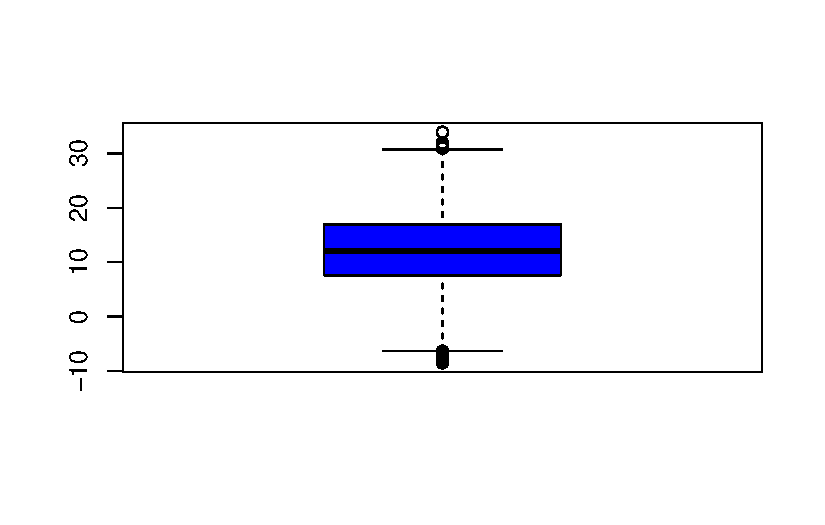
\includegraphics{RainAus_EDA_files/figure-pdf/unnamed-chunk-10-1.pdf}

}

\end{figure}

\begin{quote}
MaxTemp
\end{quote}

\begin{Shaded}
\begin{Highlighting}[]
 \FunctionTok{boxplot}\NormalTok{(weatherAusNew}\SpecialCharTok{$}\NormalTok{MaxTemp, }\AttributeTok{col =} \StringTok{"blue"}\NormalTok{, }\AttributeTok{border =} \StringTok{"black"}\NormalTok{)}
\end{Highlighting}
\end{Shaded}

\begin{figure}[H]

{\centering 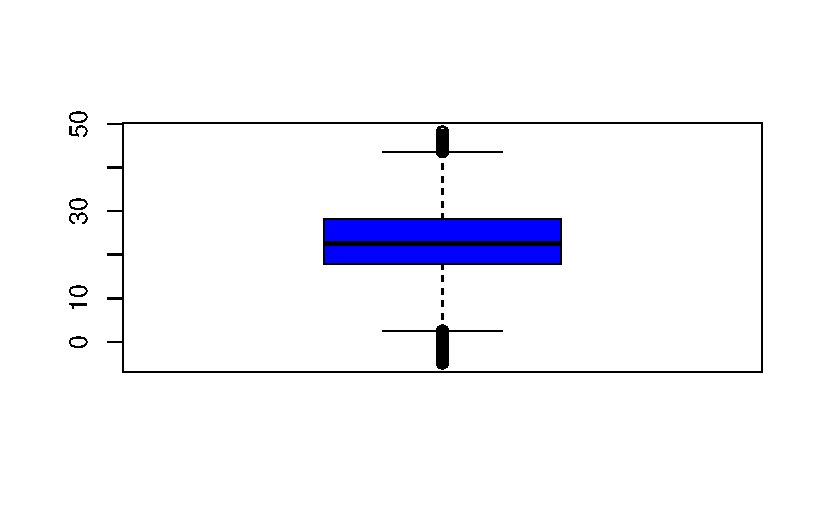
\includegraphics{RainAus_EDA_files/figure-pdf/unnamed-chunk-11-1.pdf}

}

\end{figure}

\begin{quote}
Rainfall
\end{quote}

\begin{Shaded}
\begin{Highlighting}[]
 \FunctionTok{boxplot}\NormalTok{(weatherAusNew}\SpecialCharTok{$}\NormalTok{Rainfall, }\AttributeTok{col =} \StringTok{"blue"}\NormalTok{, }\AttributeTok{border =} \StringTok{"black"}\NormalTok{)}
\end{Highlighting}
\end{Shaded}

\begin{figure}[H]

{\centering 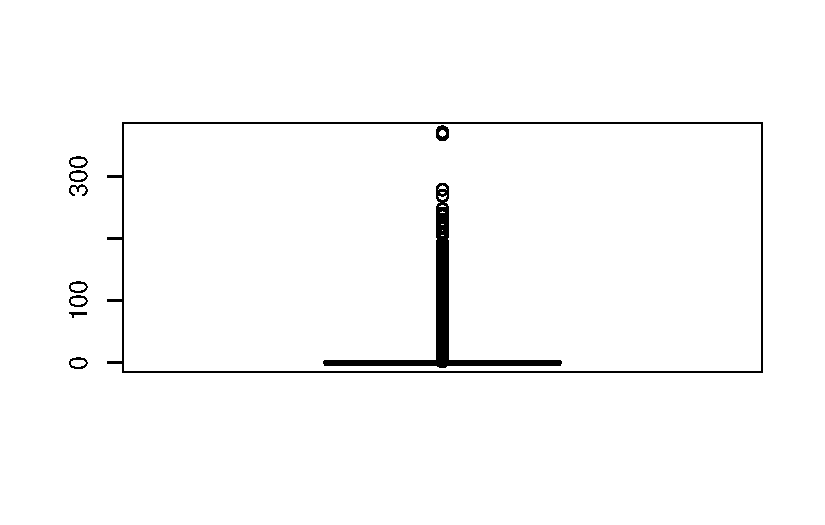
\includegraphics{RainAus_EDA_files/figure-pdf/unnamed-chunk-12-1.pdf}

}

\end{figure}

\begin{quote}
Evaporation
\end{quote}

\begin{Shaded}
\begin{Highlighting}[]
 \FunctionTok{boxplot}\NormalTok{(weatherAusNew}\SpecialCharTok{$}\NormalTok{Evaporation, }\AttributeTok{col =} \StringTok{"blue"}\NormalTok{, }\AttributeTok{border =} \StringTok{"black"}\NormalTok{)}
\end{Highlighting}
\end{Shaded}

\begin{figure}[H]

{\centering 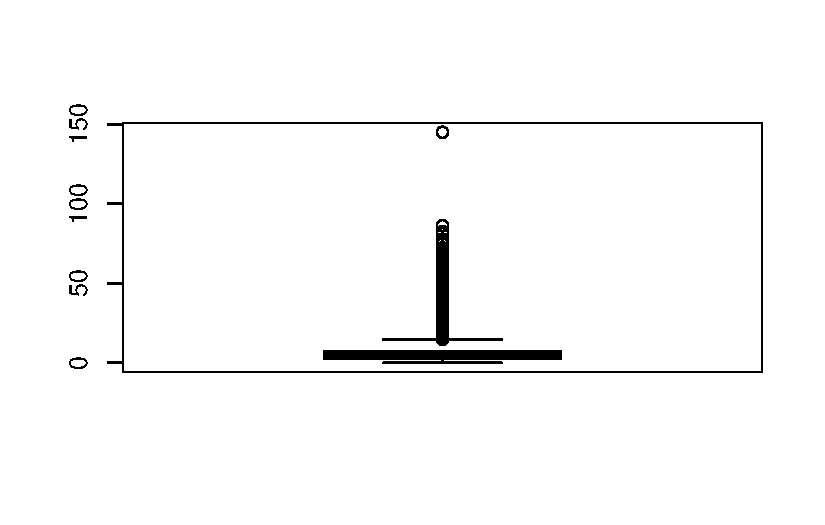
\includegraphics{RainAus_EDA_files/figure-pdf/unnamed-chunk-13-1.pdf}

}

\end{figure}

\begin{quote}
Sunshine
\end{quote}

\begin{Shaded}
\begin{Highlighting}[]
 \FunctionTok{boxplot}\NormalTok{(weatherAusNew}\SpecialCharTok{$}\NormalTok{Sunshine, }\AttributeTok{col =} \StringTok{"blue"}\NormalTok{, }\AttributeTok{border =} \StringTok{"black"}\NormalTok{)}
\end{Highlighting}
\end{Shaded}

\begin{figure}[H]

{\centering 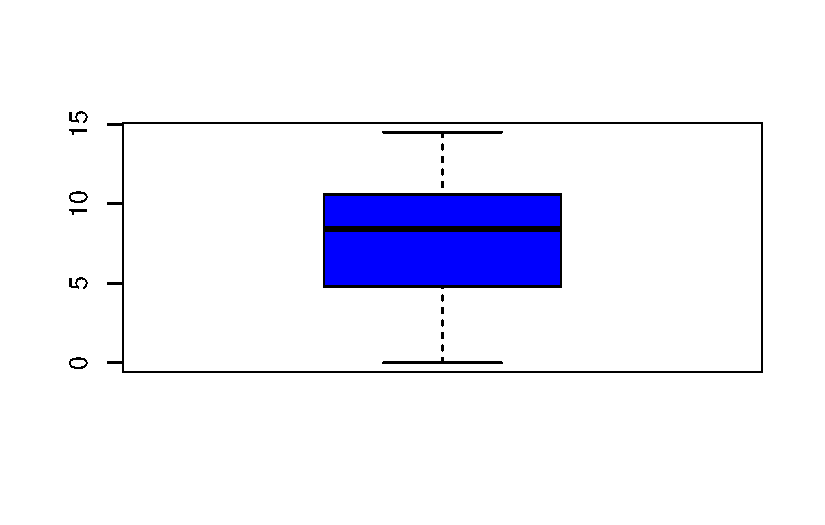
\includegraphics{RainAus_EDA_files/figure-pdf/unnamed-chunk-14-1.pdf}

}

\end{figure}

\begin{quote}
WindGustSpeed
\end{quote}

\begin{Shaded}
\begin{Highlighting}[]
 \FunctionTok{boxplot}\NormalTok{(weatherAusNew}\SpecialCharTok{$}\NormalTok{WindGustSpeed, }\AttributeTok{col =} \StringTok{"blue"}\NormalTok{, }\AttributeTok{border =} \StringTok{"black"}\NormalTok{)}
\end{Highlighting}
\end{Shaded}

\begin{figure}[H]

{\centering 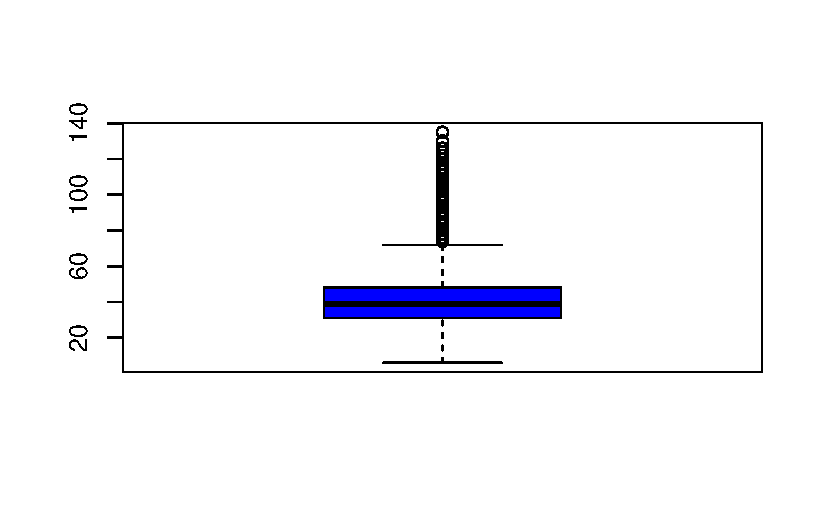
\includegraphics{RainAus_EDA_files/figure-pdf/unnamed-chunk-15-1.pdf}

}

\end{figure}

\begin{quote}
WindSpeed9am
\end{quote}

\begin{Shaded}
\begin{Highlighting}[]
 \FunctionTok{boxplot}\NormalTok{(weatherAusNew}\SpecialCharTok{$}\NormalTok{WindSpeed9am, }\AttributeTok{col =} \StringTok{"blue"}\NormalTok{, }\AttributeTok{border =} \StringTok{"black"}\NormalTok{)}
\end{Highlighting}
\end{Shaded}

\begin{figure}[H]

{\centering 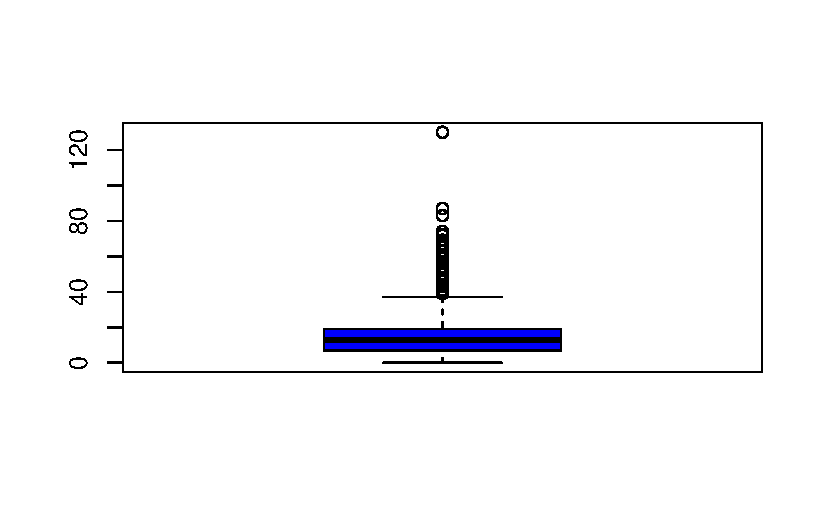
\includegraphics{RainAus_EDA_files/figure-pdf/unnamed-chunk-16-1.pdf}

}

\end{figure}

\begin{quote}
WindSpeed3pm
\end{quote}

\begin{Shaded}
\begin{Highlighting}[]
 \FunctionTok{boxplot}\NormalTok{(weatherAusNew}\SpecialCharTok{$}\NormalTok{WindSpeed3pm, }\AttributeTok{col =} \StringTok{"blue"}\NormalTok{, }\AttributeTok{border =} \StringTok{"black"}\NormalTok{)}
\end{Highlighting}
\end{Shaded}

\begin{figure}[H]

{\centering 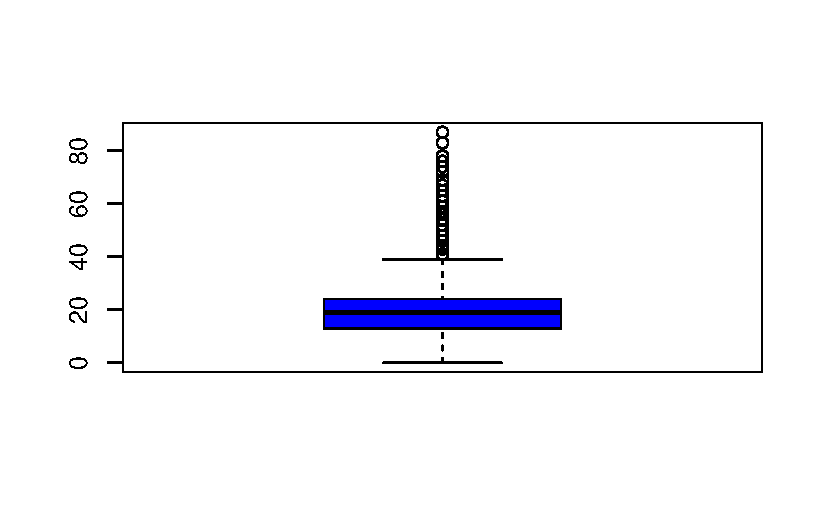
\includegraphics{RainAus_EDA_files/figure-pdf/unnamed-chunk-17-1.pdf}

}

\end{figure}

\begin{quote}
Humidity9am
\end{quote}

\begin{Shaded}
\begin{Highlighting}[]
 \FunctionTok{boxplot}\NormalTok{(weatherAusNew}\SpecialCharTok{$}\NormalTok{Humidity9am, }\AttributeTok{col =} \StringTok{"blue"}\NormalTok{, }\AttributeTok{border =} \StringTok{"black"}\NormalTok{)}
\end{Highlighting}
\end{Shaded}

\begin{figure}[H]

{\centering 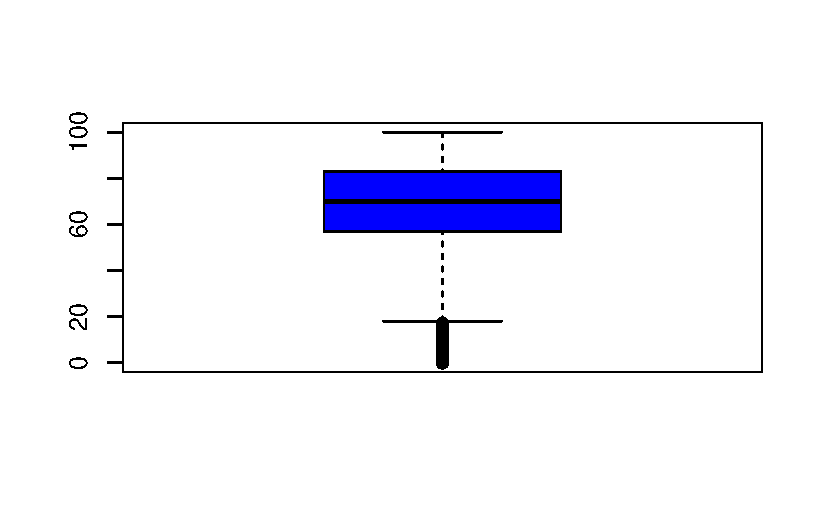
\includegraphics{RainAus_EDA_files/figure-pdf/unnamed-chunk-18-1.pdf}

}

\end{figure}

\begin{quote}
Humidity3pm
\end{quote}

\begin{Shaded}
\begin{Highlighting}[]
 \FunctionTok{boxplot}\NormalTok{(weatherAusNew}\SpecialCharTok{$}\NormalTok{Humidity3pm, }\AttributeTok{col =} \StringTok{"blue"}\NormalTok{, }\AttributeTok{border =} \StringTok{"black"}\NormalTok{)}
\end{Highlighting}
\end{Shaded}

\begin{figure}[H]

{\centering 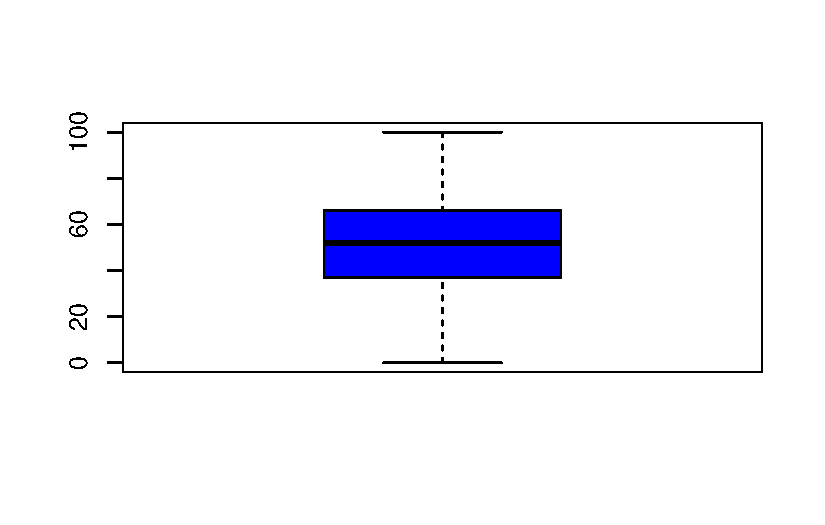
\includegraphics{RainAus_EDA_files/figure-pdf/unnamed-chunk-19-1.pdf}

}

\end{figure}

\begin{quote}
Pressure9am
\end{quote}

\begin{Shaded}
\begin{Highlighting}[]
 \FunctionTok{boxplot}\NormalTok{(weatherAusNew}\SpecialCharTok{$}\NormalTok{Pressure9am, }\AttributeTok{col =} \StringTok{"blue"}\NormalTok{, }\AttributeTok{border =} \StringTok{"black"}\NormalTok{)}
\end{Highlighting}
\end{Shaded}

\begin{figure}[H]

{\centering 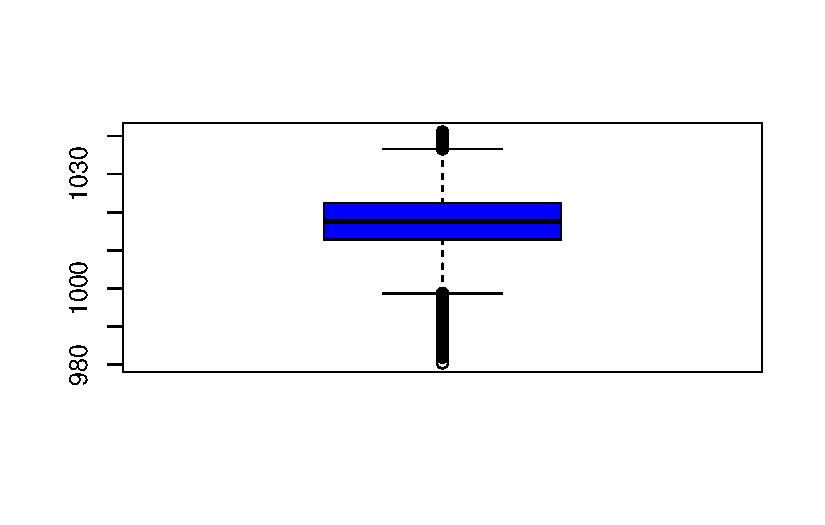
\includegraphics{RainAus_EDA_files/figure-pdf/unnamed-chunk-20-1.pdf}

}

\end{figure}

\begin{quote}
Pressure3pm
\end{quote}

\begin{Shaded}
\begin{Highlighting}[]
 \FunctionTok{boxplot}\NormalTok{(weatherAusNew}\SpecialCharTok{$}\NormalTok{Pressure3pm, }\AttributeTok{col =} \StringTok{"blue"}\NormalTok{, }\AttributeTok{border =} \StringTok{"black"}\NormalTok{)}
\end{Highlighting}
\end{Shaded}

\begin{figure}[H]

{\centering 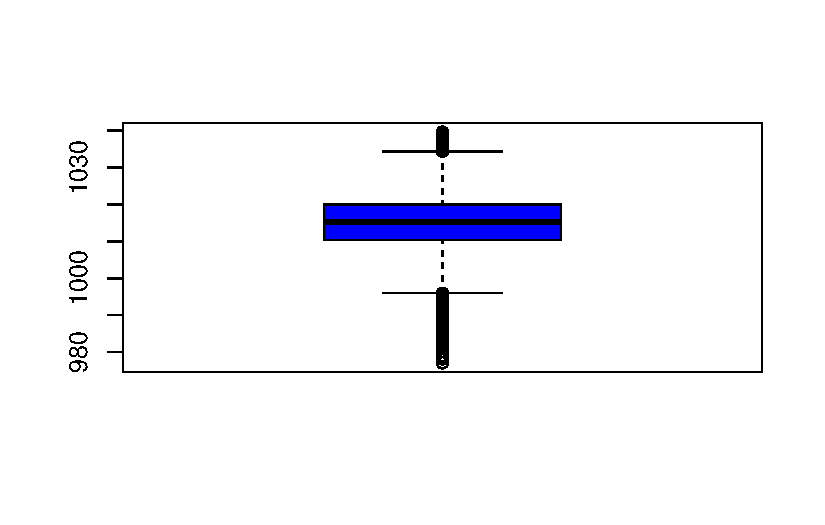
\includegraphics{RainAus_EDA_files/figure-pdf/unnamed-chunk-21-1.pdf}

}

\end{figure}

\begin{quote}
Cloud9am
\end{quote}

\begin{Shaded}
\begin{Highlighting}[]
 \FunctionTok{boxplot}\NormalTok{(weatherAusNew}\SpecialCharTok{$}\NormalTok{Cloud9am, }\AttributeTok{col =} \StringTok{"blue"}\NormalTok{, }\AttributeTok{border =} \StringTok{"black"}\NormalTok{)}
\end{Highlighting}
\end{Shaded}

\begin{figure}[H]

{\centering 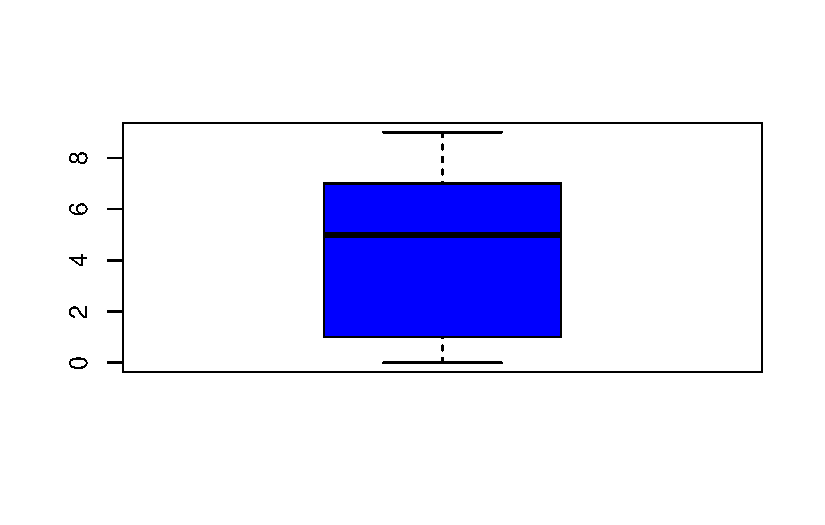
\includegraphics{RainAus_EDA_files/figure-pdf/unnamed-chunk-22-1.pdf}

}

\end{figure}

\begin{quote}
Cloud3pm
\end{quote}

\begin{Shaded}
\begin{Highlighting}[]
 \FunctionTok{boxplot}\NormalTok{(weatherAusNew}\SpecialCharTok{$}\NormalTok{Cloud3pm, }\AttributeTok{col =} \StringTok{"blue"}\NormalTok{, }\AttributeTok{border =} \StringTok{"black"}\NormalTok{)}
\end{Highlighting}
\end{Shaded}

\begin{figure}[H]

{\centering 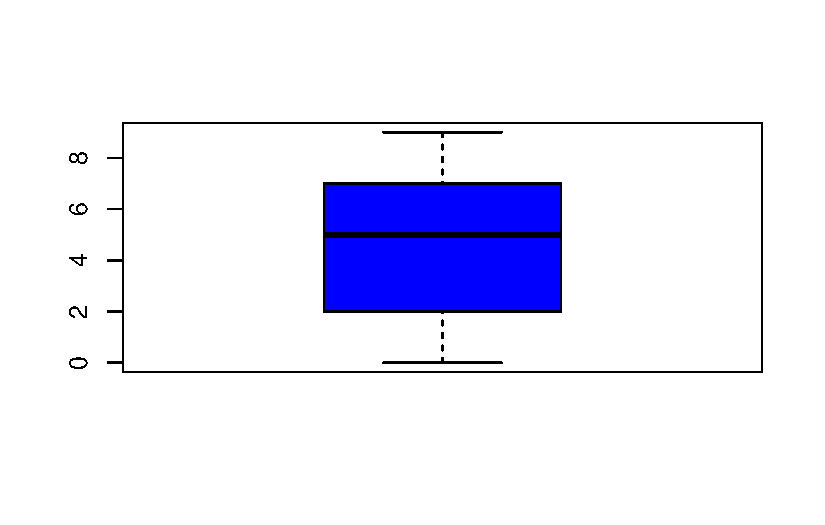
\includegraphics{RainAus_EDA_files/figure-pdf/unnamed-chunk-23-1.pdf}

}

\end{figure}

\begin{quote}
Temp9am
\end{quote}

\begin{Shaded}
\begin{Highlighting}[]
 \FunctionTok{boxplot}\NormalTok{(weatherAusNew}\SpecialCharTok{$}\NormalTok{Temp9am, }\AttributeTok{col =} \StringTok{"blue"}\NormalTok{, }\AttributeTok{border =} \StringTok{"black"}\NormalTok{)}
\end{Highlighting}
\end{Shaded}

\begin{figure}[H]

{\centering 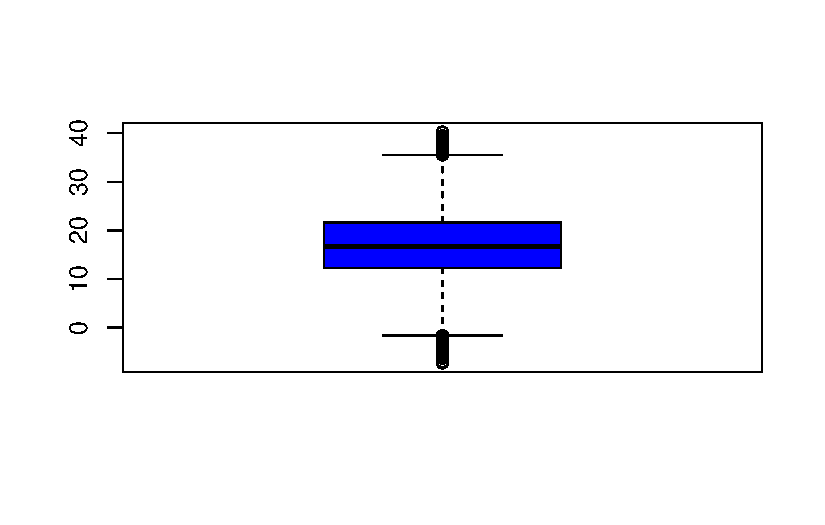
\includegraphics{RainAus_EDA_files/figure-pdf/unnamed-chunk-24-1.pdf}

}

\end{figure}

\begin{quote}
Temp3pm
\end{quote}

\begin{Shaded}
\begin{Highlighting}[]
 \FunctionTok{boxplot}\NormalTok{(weatherAusNew}\SpecialCharTok{$}\NormalTok{Temp3pm, }\AttributeTok{col =} \StringTok{"blue"}\NormalTok{, }\AttributeTok{border =} \StringTok{"black"}\NormalTok{)}
\end{Highlighting}
\end{Shaded}

\begin{figure}[H]

{\centering 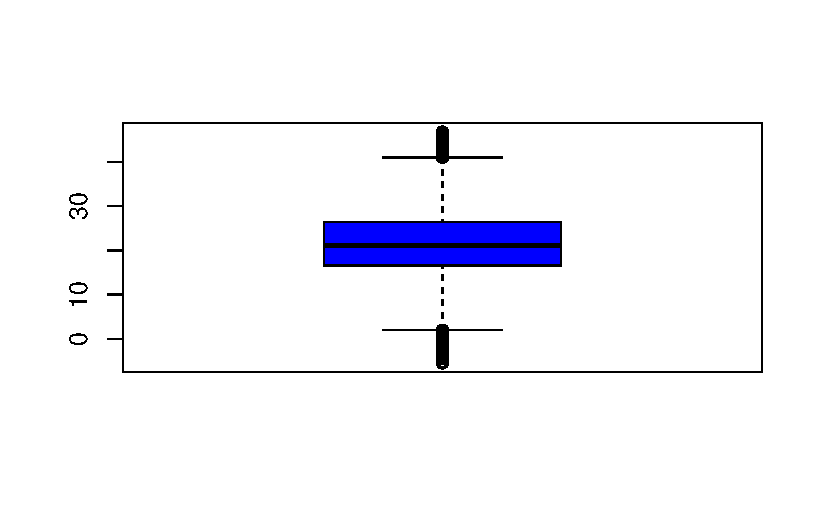
\includegraphics{RainAus_EDA_files/figure-pdf/unnamed-chunk-25-1.pdf}

}

\end{figure}

\begin{quote}
Year
\end{quote}

\begin{Shaded}
\begin{Highlighting}[]
 \FunctionTok{boxplot}\NormalTok{(weatherAusNew}\SpecialCharTok{$}\NormalTok{Year, }\AttributeTok{col =} \StringTok{"blue"}\NormalTok{, }\AttributeTok{border =} \StringTok{"black"}\NormalTok{)}
\end{Highlighting}
\end{Shaded}

\begin{figure}[H]

{\centering 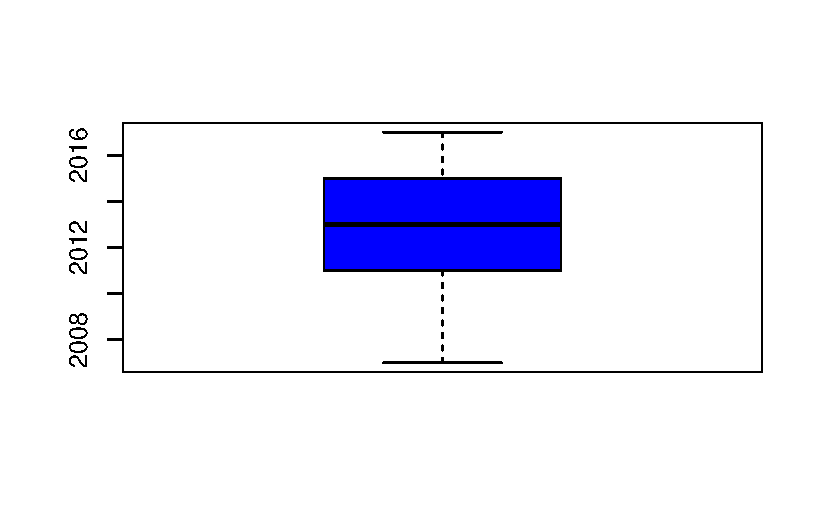
\includegraphics{RainAus_EDA_files/figure-pdf/unnamed-chunk-26-1.pdf}

}

\end{figure}

\begin{quote}
Month
\end{quote}

\begin{Shaded}
\begin{Highlighting}[]
 \FunctionTok{boxplot}\NormalTok{(weatherAusNew}\SpecialCharTok{$}\NormalTok{Month, }\AttributeTok{col =} \StringTok{"blue"}\NormalTok{, }\AttributeTok{border =} \StringTok{"black"}\NormalTok{)}
\end{Highlighting}
\end{Shaded}

\begin{figure}[H]

{\centering 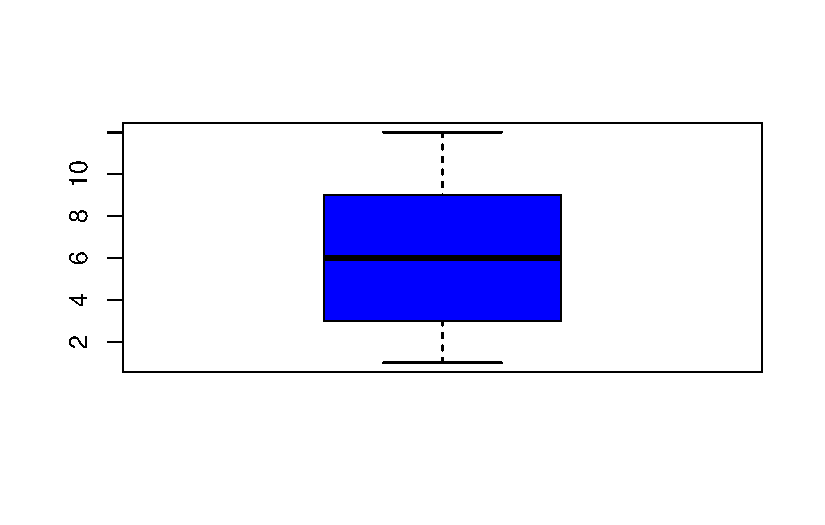
\includegraphics{RainAus_EDA_files/figure-pdf/unnamed-chunk-27-1.pdf}

}

\end{figure}

\begin{quote}
Day
\end{quote}

\begin{Shaded}
\begin{Highlighting}[]
 \FunctionTok{boxplot}\NormalTok{(weatherAusNew}\SpecialCharTok{$}\NormalTok{Day, }\AttributeTok{col =} \StringTok{"blue"}\NormalTok{, }\AttributeTok{border =} \StringTok{"black"}\NormalTok{)}
\end{Highlighting}
\end{Shaded}

\begin{figure}[H]

{\centering 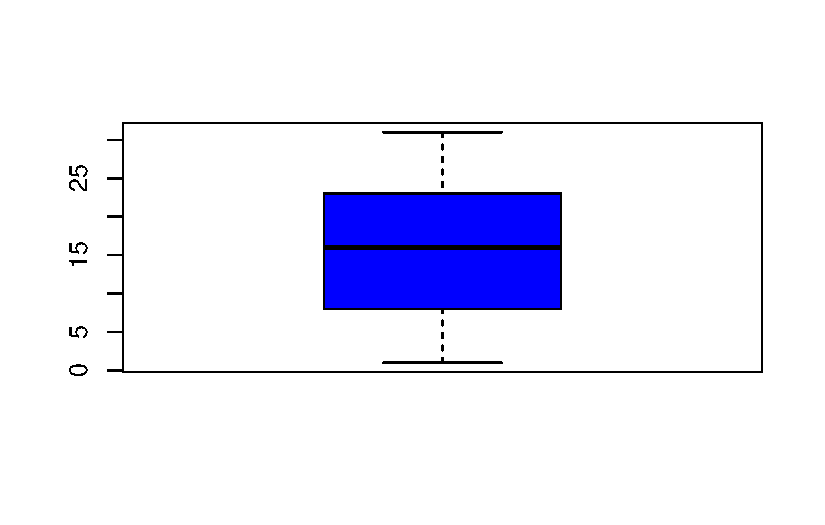
\includegraphics{RainAus_EDA_files/figure-pdf/unnamed-chunk-28-1.pdf}

}

\end{figure}

\hypertarget{multicollinearity}{%
\subsubsection{Multicollinearity}\label{multicollinearity}}

\begin{Shaded}
\begin{Highlighting}[]
\NormalTok{weatherAusNew }\SpecialCharTok{\%\textgreater{}\%} \FunctionTok{select}\NormalTok{(}\FunctionTok{where}\NormalTok{(is.numeric)) }\SpecialCharTok{\%\textgreater{}\%} \FunctionTok{model.matrix}\NormalTok{(}\SpecialCharTok{\textasciitilde{}}\DecValTok{0}\SpecialCharTok{+}\NormalTok{.,}
              \AttributeTok{data=}\NormalTok{.) }\SpecialCharTok{\%\textgreater{}\%}
    \FunctionTok{cor}\NormalTok{(}\AttributeTok{use=}\StringTok{"pairwise.complete.obs"}\NormalTok{) }\SpecialCharTok{\%\textgreater{}\%} 
    \FunctionTok{ggcorrplot}\NormalTok{(}\AttributeTok{show.diag =} \ConstantTok{FALSE}\NormalTok{, }\AttributeTok{type=}\StringTok{"full"}\NormalTok{,}
               \AttributeTok{lab=}\ConstantTok{TRUE}\NormalTok{,}\AttributeTok{legend.title =} \StringTok{"Correlation"}\NormalTok{ ,lab\_size}
               \OtherTok{=} \DecValTok{2}\NormalTok{,}\AttributeTok{lab\_col =} \StringTok{"black"}\NormalTok{ ,}\AttributeTok{ggtheme =}
\NormalTok{                 ggplot2}\SpecialCharTok{::}\NormalTok{theme\_gray,}
               \AttributeTok{colors =} \FunctionTok{c}\NormalTok{(}\StringTok{"white"}\NormalTok{,}\StringTok{"green"}\NormalTok{,}\StringTok{"darkgreen"}\NormalTok{),}
               \AttributeTok{outline.color =} \StringTok{"black"}\NormalTok{)}

\FunctionTok{write.csv}\NormalTok{(weatherAusNew, }\AttributeTok{file =} \StringTok{"weatherNewToPython.csv"}\NormalTok{, }\AttributeTok{row.names =} \ConstantTok{FALSE}\NormalTok{)}
\FunctionTok{colnames}\NormalTok{(weatherAusNew)}
\end{Highlighting}
\end{Shaded}

\begin{verbatim}
 [1] "Location"      "MinTemp"       "MaxTemp"       "Rainfall"     
 [5] "Evaporation"   "Sunshine"      "WindGustDir"   "WindGustSpeed"
 [9] "WindDir9am"    "WindDir3pm"    "WindSpeed9am"  "WindSpeed3pm" 
[13] "Humidity9am"   "Humidity3pm"   "Pressure9am"   "Pressure3pm"  
[17] "Cloud9am"      "Cloud3pm"      "Temp9am"       "Temp3pm"      
[21] "RainToday"     "RainTomorrow"  "Year"          "Month"        
[25] "Day"          
\end{verbatim}

\begin{figure}[H]

{\centering 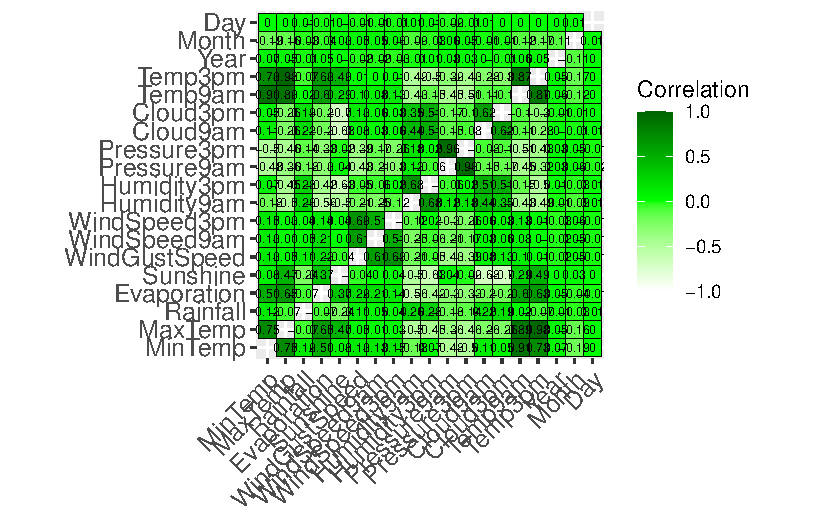
\includegraphics{RainAus_EDA_files/figure-pdf/fig-absences-1.pdf}

}

\caption{\label{fig-absences}Correlation Heatmap}

\end{figure}

\hypertarget{outliers-missing-values}{%
\paragraph{Outliers \& Missing Values}\label{outliers-missing-values}}

\begin{quote}
Outliers
\end{quote}

After drawing a boxplot for each numerical attribute in the dataset, we
compared the mean of each column with the min/max value and we have
noticed that that attributes \textbf{Rainfall}, \textbf{Evaporation},
\textbf{WindSpeed9am} and \textbf{WindSpeed3pm} might have a large
number of outliers as there's a considerable difference between average
value and max value. This also can be seen from their plots, as there is
a huge amount of points (values) that differ from the average.\\
Outliers can be identified by using some visualization tools as we have
seen above, or also with some statistical methods. Once detected,
outliers can be addressed by removing them, transforming the data, or
using robust models less sensitive to outliers.

When implementing the models, we will split the dataset into training
and testing sets. The training set will be used to train machine
learning models, allowing the algorithms to learn from the data. The
testing set, on the other hand, will be used to evaluate the models'
performance on unseen data, ensuring that the models generalize well and
provide accurate predictions in real-world scenarios.

\begin{quote}
Missing Values
\end{quote}

Addressing missing values is crucial during data preprocessing. Missing
values can result from data entry errors, collection issues, and they
can degrade performance. Because of this we are going to impute the
missing values at each implementation of the three models.
\textbf{Missing values in categorical columns} will be filled up using
the Python function \textbf{mode()} that fills in the cells with the
most common/occuring element from all other instances. \textbf{Missing
values in numerical columns} will be filled up with the median value
from all the values of the other instances.

\begin{center}\rule{0.5\linewidth}{0.5pt}\end{center}

\hypertarget{modeling}{%
\subsection{Modeling}\label{modeling}}

After performing the Exploratory Data Analysis, we will proceed to the
modeling part. In this phase we will implement three models:
\textbf{Artificial Neural Network}, \textbf{CatBoost}, and
\textbf{Logistic Regression}.

Till now the analysis was made using code chunks performed in R
langauge. For this implementation part the models will be implemented in
Python.

\hypertarget{artificial-neural-network}{%
\subsubsection{Artificial Neural
Network}\label{artificial-neural-network}}

\begin{itemize}
\item
  The ANN model derives from Biological neural networks that have the
  structure of the human brain. It contains neurons(nodes)
  interconnected to one another in various layers of the network. It
  consists of three layers: Input layer, Hidden layers (can be several
  of them) and Output layer. The input layer accepts inputs in several
  formats, the hidden layer is in-between the inputs and outputs and
  performs calculations to find hidden features and patterns. The output
  layer outputs the results of calculations.

  \begin{figure}

  {\centering 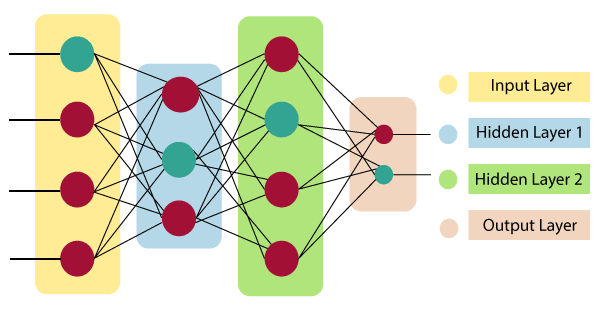
\includegraphics{ANNPicture.png}

  }

  \caption{ANN layers}

  \end{figure}
\end{itemize}

\hfill\break

\begin{itemize}
\item
  \emph{ADVANTAGES}

  \begin{itemize}
  \item
    \textbf{Parallel processing}
  \item
    Information can produce \textbf{output} even with \textbf{inadequate
    data}
  \item
    \textbf{Success} proportional to \textbf{chosen instances}
  \end{itemize}
\item
  \emph{DISADVANTAGES}

  \begin{itemize}
  \item
    Depends on \textbf{hardware}
  \item
    ANNs work with \textbf{numerical data}
  \item
    Duration of network is \textbf{unknown}
  \end{itemize}
\item
  \textbf{FUNCTIONING}

  Each input is multiplied by its corresponding weights (strength of
  interconnections between neurons). All weighted inputs are summarized
  inside the computing unit. Each neuron has its \textbf{bias,} which is
  added to the weighted sum to make it non-zero, so the total sum of
  weighted inputs can be from 0 to plus infinity. The maximum value is
  \textbf{benchmarked} to keep the response in the limits. This is
  performed in \emph{TRANSFER FUNCTIONS.}

  \emph{ACTIVATION FUNCTIONS} choose whether a node should fire or not.
  Only those who are \emph{fired} make it to the output layer.
  Activation functions are distinctive depending on the task that is
  performed.
\item
  \textbf{FEED-BACK}

  \begin{itemize}
  \tightlist
  \item
    Feed-back networks feed information back to itself
  \end{itemize}
\item
  \textbf{FEED-FORWARD}

  \begin{itemize}
  \item
    Assessment of ouputs by reviewing its inputs
  \item
    Input --\textgreater{} Neuron layer --\textgreater{} Output
  \end{itemize}
\end{itemize}

\begin{center}\rule{0.5\linewidth}{0.5pt}\end{center}

\begin{Shaded}
\begin{Highlighting}[]
\CommentTok{\# ANN IMPLEMENTATIONN}
\ImportTok{import}\NormalTok{ pandas }\ImportTok{as}\NormalTok{ pd}
\ImportTok{import}\NormalTok{ numpy }\ImportTok{as}\NormalTok{ np}
\ImportTok{import}\NormalTok{ seaborn }\ImportTok{as}\NormalTok{ sns}
\ImportTok{from}\NormalTok{ catboost }\ImportTok{import}\NormalTok{ CatBoostClassifier, Pool}
\ImportTok{from}\NormalTok{ sklearn.impute }\ImportTok{import}\NormalTok{ SimpleImputer}
\ImportTok{from}\NormalTok{ sklearn.compose }\ImportTok{import}\NormalTok{ ColumnTransformer}
\ImportTok{from}\NormalTok{ sklearn.pipeline }\ImportTok{import}\NormalTok{ Pipeline}
\ImportTok{from}\NormalTok{ sklearn.linear\_model }\ImportTok{import}\NormalTok{ LogisticRegression}
\ImportTok{from}\NormalTok{ matplotlib }\ImportTok{import}\NormalTok{ pyplot }\ImportTok{as}\NormalTok{ plt}
\ImportTok{from}\NormalTok{ sklearn.model\_selection }\ImportTok{import}\NormalTok{ train\_test\_split}
\ImportTok{from}\NormalTok{ sklearn.metrics }\ImportTok{import}\NormalTok{ classification\_report, confusion\_matrix, accuracy\_score}
\ImportTok{from}\NormalTok{ sklearn.preprocessing }\ImportTok{import}\NormalTok{ StandardScaler}
\ImportTok{from}\NormalTok{ keras.layers }\ImportTok{import}\NormalTok{ Dense, BatchNormalization, Dropout}
\ImportTok{from}\NormalTok{ keras.models }\ImportTok{import}\NormalTok{ Sequential}
\ImportTok{from}\NormalTok{ keras }\ImportTok{import}\NormalTok{ callbacks}
\ImportTok{from}\NormalTok{ keras.optimizers }\ImportTok{import}\NormalTok{ Adam}
\ImportTok{from}\NormalTok{ sklearn.preprocessing }\ImportTok{import}\NormalTok{ LabelEncoder, StandardScaler, OneHotEncoder}

\NormalTok{df }\OperatorTok{=}\NormalTok{ pd.read\_csv(}\StringTok{\textquotesingle{}weatherNewToPython.csv\textquotesingle{}}\NormalTok{)}

\CommentTok{\# Categorical columns}
\NormalTok{s }\OperatorTok{=}\NormalTok{ (df.dtypes }\OperatorTok{==} \StringTok{"object"}\NormalTok{)}
\NormalTok{cat\_cols }\OperatorTok{=} \BuiltInTok{list}\NormalTok{(s[s].index)}

\BuiltInTok{print}\NormalTok{(}\StringTok{"Categorial variables"}\NormalTok{)}
\end{Highlighting}
\end{Shaded}

\begin{verbatim}
Categorial variables
\end{verbatim}

\begin{Shaded}
\begin{Highlighting}[]
\BuiltInTok{print}\NormalTok{(cat\_cols)}
\end{Highlighting}
\end{Shaded}

\begin{verbatim}
['Location', 'WindGustDir', 'WindDir9am', 'WindDir3pm', 'RainToday', 'RainTomorrow']
\end{verbatim}

\begin{Shaded}
\begin{Highlighting}[]
\ControlFlowTok{for}\NormalTok{ cols }\KeywordTok{in}\NormalTok{ cat\_cols:}
    
\NormalTok{    df[cols] }\OperatorTok{=}\NormalTok{ df[cols].fillna(df[cols].mode()[}\DecValTok{0}\NormalTok{])}

\CommentTok{\# Numerical columns}
\NormalTok{t }\OperatorTok{=}\NormalTok{ (df.dtypes }\OperatorTok{==} \StringTok{"float64"}\NormalTok{)}
\NormalTok{num\_cols }\OperatorTok{=} \BuiltInTok{list}\NormalTok{(t[t].index)}

\BuiltInTok{print}\NormalTok{(}\StringTok{"Numeric variables:"}\NormalTok{)}
\end{Highlighting}
\end{Shaded}

\begin{verbatim}
Numeric variables:
\end{verbatim}

\begin{Shaded}
\begin{Highlighting}[]
\BuiltInTok{print}\NormalTok{(num\_cols)}
\end{Highlighting}
\end{Shaded}

\begin{verbatim}
['MinTemp', 'MaxTemp', 'Rainfall', 'Evaporation', 'Sunshine', 'WindGustSpeed', 'WindSpeed9am', 'WindSpeed3pm', 'Humidity9am', 'Humidity3pm', 'Pressure9am', 'Pressure3pm', 'Cloud9am', 'Cloud3pm', 'Temp9am', 'Temp3pm']
\end{verbatim}

\begin{Shaded}
\begin{Highlighting}[]
\ControlFlowTok{for}\NormalTok{ cols }\KeywordTok{in}\NormalTok{ num\_cols:}
    
\NormalTok{    df[cols] }\OperatorTok{=}\NormalTok{ df[cols].fillna(df[cols].median())}
\NormalTok{df.info()}
\end{Highlighting}
\end{Shaded}

\begin{verbatim}
<class 'pandas.core.frame.DataFrame'>
RangeIndex: 145460 entries, 0 to 145459
Data columns (total 25 columns):
 #   Column         Non-Null Count   Dtype  
---  ------         --------------   -----  
 0   Location       145460 non-null  object 
 1   MinTemp        145460 non-null  float64
 2   MaxTemp        145460 non-null  float64
 3   Rainfall       145460 non-null  float64
 4   Evaporation    145460 non-null  float64
 5   Sunshine       145460 non-null  float64
 6   WindGustDir    145460 non-null  object 
 7   WindGustSpeed  145460 non-null  float64
 8   WindDir9am     145460 non-null  object 
 9   WindDir3pm     145460 non-null  object 
 10  WindSpeed9am   145460 non-null  float64
 11  WindSpeed3pm   145460 non-null  float64
 12  Humidity9am    145460 non-null  float64
 13  Humidity3pm    145460 non-null  float64
 14  Pressure9am    145460 non-null  float64
 15  Pressure3pm    145460 non-null  float64
 16  Cloud9am       145460 non-null  float64
 17  Cloud3pm       145460 non-null  float64
 18  Temp9am        145460 non-null  float64
 19  Temp3pm        145460 non-null  float64
 20  RainToday      145460 non-null  object 
 21  RainTomorrow   145460 non-null  object 
 22  Year           145460 non-null  int64  
 23  Month          145460 non-null  int64  
 24  Day            145460 non-null  int64  
dtypes: float64(16), int64(3), object(6)
memory usage: 27.7+ MB
\end{verbatim}

\begin{Shaded}
\begin{Highlighting}[]
\NormalTok{df.head(}\DecValTok{10}\NormalTok{)}
\end{Highlighting}
\end{Shaded}

\begin{verbatim}
  Location  MinTemp  MaxTemp  Rainfall  ...  RainTomorrow  Year Month  Day
0   Albury     13.4     22.9       0.6  ...            No  2008    12    1
1   Albury      7.4     25.1       0.0  ...            No  2008    12    2
2   Albury     12.9     25.7       0.0  ...            No  2008    12    3
3   Albury      9.2     28.0       0.0  ...            No  2008    12    4
4   Albury     17.5     32.3       1.0  ...            No  2008    12    5
5   Albury     14.6     29.7       0.2  ...            No  2008    12    6
6   Albury     14.3     25.0       0.0  ...            No  2008    12    7
7   Albury      7.7     26.7       0.0  ...            No  2008    12    8
8   Albury      9.7     31.9       0.0  ...           Yes  2008    12    9
9   Albury     13.1     30.1       1.4  ...            No  2008    12   10

[10 rows x 25 columns]
\end{verbatim}

\begin{Shaded}
\begin{Highlighting}[]
\CommentTok{\# Categorical columns of type "object" into "float64"}
\NormalTok{label\_encoder }\OperatorTok{=}\NormalTok{ LabelEncoder()}
\ControlFlowTok{for}\NormalTok{ cols }\KeywordTok{in}\NormalTok{ cat\_cols: }
\NormalTok{    df[cols] }\OperatorTok{=}\NormalTok{ label\_encoder.fit\_transform(df[cols])}

    
\NormalTok{df.info()}
\end{Highlighting}
\end{Shaded}

\begin{verbatim}
<class 'pandas.core.frame.DataFrame'>
RangeIndex: 145460 entries, 0 to 145459
Data columns (total 25 columns):
 #   Column         Non-Null Count   Dtype  
---  ------         --------------   -----  
 0   Location       145460 non-null  int32  
 1   MinTemp        145460 non-null  float64
 2   MaxTemp        145460 non-null  float64
 3   Rainfall       145460 non-null  float64
 4   Evaporation    145460 non-null  float64
 5   Sunshine       145460 non-null  float64
 6   WindGustDir    145460 non-null  int32  
 7   WindGustSpeed  145460 non-null  float64
 8   WindDir9am     145460 non-null  int32  
 9   WindDir3pm     145460 non-null  int32  
 10  WindSpeed9am   145460 non-null  float64
 11  WindSpeed3pm   145460 non-null  float64
 12  Humidity9am    145460 non-null  float64
 13  Humidity3pm    145460 non-null  float64
 14  Pressure9am    145460 non-null  float64
 15  Pressure3pm    145460 non-null  float64
 16  Cloud9am       145460 non-null  float64
 17  Cloud3pm       145460 non-null  float64
 18  Temp9am        145460 non-null  float64
 19  Temp3pm        145460 non-null  float64
 20  RainToday      145460 non-null  int32  
 21  RainTomorrow   145460 non-null  int32  
 22  Year           145460 non-null  int64  
 23  Month          145460 non-null  int64  
 24  Day            145460 non-null  int64  
dtypes: float64(16), int32(6), int64(3)
memory usage: 24.4 MB
\end{verbatim}

\begin{Shaded}
\begin{Highlighting}[]
\CommentTok{\# dropping target and extra columns}
\NormalTok{features }\OperatorTok{=}\NormalTok{ df.drop([}\StringTok{\textquotesingle{}RainTomorrow\textquotesingle{}}\NormalTok{, }\StringTok{\textquotesingle{}Year\textquotesingle{}}\NormalTok{,}\StringTok{\textquotesingle{}Month\textquotesingle{}}\NormalTok{, }\StringTok{\textquotesingle{}Day\textquotesingle{}}\NormalTok{], axis}\OperatorTok{=}\DecValTok{1}\NormalTok{) }
\NormalTok{target }\OperatorTok{=}\NormalTok{ df[}\StringTok{\textquotesingle{}RainTomorrow\textquotesingle{}}\NormalTok{]}

\NormalTok{X }\OperatorTok{=}\NormalTok{ features}
\NormalTok{y }\OperatorTok{=}\NormalTok{ target}

\CommentTok{\# Splitting test and training sets}
\NormalTok{X\_train, X\_test, y\_train, y\_test }\OperatorTok{=}\NormalTok{ train\_test\_split(X, y, test\_size }\OperatorTok{=} \FloatTok{0.2}\NormalTok{, random\_state }\OperatorTok{=} \DecValTok{42}\NormalTok{)}

\NormalTok{X.shape}
\end{Highlighting}
\end{Shaded}

\begin{verbatim}
(145460, 21)
\end{verbatim}

\begin{Shaded}
\begin{Highlighting}[]
\CommentTok{\#Early stopping}
\NormalTok{early\_stopping }\OperatorTok{=}\NormalTok{ callbacks.EarlyStopping(}
\NormalTok{    min\_delta}\OperatorTok{=}\FloatTok{0.001}\NormalTok{, }\CommentTok{\# minimium amount of change to count as an improvement}
\NormalTok{    patience}\OperatorTok{=}\DecValTok{20}\NormalTok{, }\CommentTok{\# how many epochs to wait before stopping}
\NormalTok{    restore\_best\_weights}\OperatorTok{=}\VariableTok{True}\NormalTok{,}
\NormalTok{)}

\CommentTok{\# Initialising the Neural Network}
\NormalTok{model }\OperatorTok{=}\NormalTok{ Sequential()}

\CommentTok{\# Adding layers to the network}
\NormalTok{model.add(Dense(units }\OperatorTok{=} \DecValTok{32}\NormalTok{, kernel\_initializer }\OperatorTok{=} \StringTok{\textquotesingle{}uniform\textquotesingle{}}\NormalTok{, activation }\OperatorTok{=} \StringTok{\textquotesingle{}relu\textquotesingle{}}\NormalTok{, input\_dim }\OperatorTok{=} \DecValTok{21}\NormalTok{))}
\NormalTok{model.add(Dense(units }\OperatorTok{=} \DecValTok{32}\NormalTok{, kernel\_initializer }\OperatorTok{=} \StringTok{\textquotesingle{}uniform\textquotesingle{}}\NormalTok{, activation }\OperatorTok{=} \StringTok{\textquotesingle{}relu\textquotesingle{}}\NormalTok{))}
\NormalTok{model.add(Dense(units }\OperatorTok{=} \DecValTok{16}\NormalTok{, kernel\_initializer }\OperatorTok{=} \StringTok{\textquotesingle{}uniform\textquotesingle{}}\NormalTok{, activation }\OperatorTok{=} \StringTok{\textquotesingle{}relu\textquotesingle{}}\NormalTok{))}
\NormalTok{model.add(Dropout(}\FloatTok{0.25}\NormalTok{))}
\NormalTok{model.add(Dense(units }\OperatorTok{=} \DecValTok{8}\NormalTok{, kernel\_initializer }\OperatorTok{=} \StringTok{\textquotesingle{}uniform\textquotesingle{}}\NormalTok{, activation }\OperatorTok{=} \StringTok{\textquotesingle{}relu\textquotesingle{}}\NormalTok{))}
\NormalTok{model.add(Dropout(}\FloatTok{0.5}\NormalTok{))}
\NormalTok{model.add(Dense(units }\OperatorTok{=} \DecValTok{1}\NormalTok{, kernel\_initializer }\OperatorTok{=} \StringTok{\textquotesingle{}uniform\textquotesingle{}}\NormalTok{, activation }\OperatorTok{=} \StringTok{\textquotesingle{}sigmoid\textquotesingle{}}\NormalTok{))}

\CommentTok{\# Compiling the ANN}
\NormalTok{opt }\OperatorTok{=}\NormalTok{ Adam(learning\_rate}\OperatorTok{=}\FloatTok{0.001}\NormalTok{)}
\NormalTok{model.}\BuiltInTok{compile}\NormalTok{(optimizer }\OperatorTok{=}\NormalTok{ opt, loss }\OperatorTok{=} \StringTok{\textquotesingle{}binary\_crossentropy\textquotesingle{}}\NormalTok{, metrics }\OperatorTok{=}\NormalTok{ [}\StringTok{\textquotesingle{}accuracy\textquotesingle{}}\NormalTok{])}

\CommentTok{\# Train the ANN}
\NormalTok{history }\OperatorTok{=}\NormalTok{ model.fit(X\_train, y\_train, batch\_size }\OperatorTok{=} \DecValTok{32}\NormalTok{, epochs }\OperatorTok{=} \DecValTok{150}\NormalTok{, callbacks}\OperatorTok{=}\NormalTok{[early\_stopping], validation\_split}\OperatorTok{=}\FloatTok{0.2}\NormalTok{)}
\end{Highlighting}
\end{Shaded}

\begin{verbatim}
Epoch 1/150

   1/2910 ━━━━━━━━━━━━━━━━━━━━ 1:02:09 1s/step - accuracy: 0.3125 - loss: 0.6933
  43/2910 ━━━━━━━━━━━━━━━━━━━━ 3s 1ms/step - accuracy: 0.7393 - loss: 0.6680    
  99/2910 ━━━━━━━━━━━━━━━━━━━━ 2s 1ms/step - accuracy: 0.7683 - loss: 0.6172
 155/2910 ━━━━━━━━━━━━━━━━━━━━ 2s 986us/step - accuracy: 0.7768 - loss: 0.5959
 216/2910 ━━━━━━━━━━━━━━━━━━━━ 2s 946us/step - accuracy: 0.7803 - loss: 0.5838
 268/2910 ━━━━━━━━━━━━━━━━━━━━ 2s 952us/step - accuracy: 0.7820 - loss: 0.5767
 321/2910 ━━━━━━━━━━━━━━━━━━━━ 2s 955us/step - accuracy: 0.7832 - loss: 0.5712
 365/2910 ━━━━━━━━━━━━━━━━━━━━ 2s 977us/step - accuracy: 0.7837 - loss: 0.5673
 407/2910 ━━━━━━━━━━━━━━━━━━━━ 2s 1ms/step - accuracy: 0.7840 - loss: 0.5636  
 457/2910 ━━━━━━━━━━━━━━━━━━━━ 2s 1ms/step - accuracy: 0.7841 - loss: 0.5593
 511/2910 ━━━━━━━━━━━━━━━━━━━━ 2s 997us/step - accuracy: 0.7841 - loss: 0.5547
 567/2910 ━━━━━━━━━━━━━━━━━━━━ 2s 988us/step - accuracy: 0.7840 - loss: 0.5502
 614/2910 ━━━━━━━━━━━━━━━━━━━━ 2s 995us/step - accuracy: 0.7838 - loss: 0.5467
 652/2910 ━━━━━━━━━━━━━━━━━━━━ 2s 1ms/step - accuracy: 0.7836 - loss: 0.5440  
 688/2910 ━━━━━━━━━━━━━━━━━━━━ 2s 1ms/step - accuracy: 0.7835 - loss: 0.5416
 723/2910 ━━━━━━━━━━━━━━━━━━━━ 2s 1ms/step - accuracy: 0.7833 - loss: 0.5394
 757/2910 ━━━━━━━━━━━━━━━━━━━━ 2s 1ms/step - accuracy: 0.7832 - loss: 0.5373
 792/2910 ━━━━━━━━━━━━━━━━━━━━ 2s 1ms/step - accuracy: 0.7831 - loss: 0.5352
 830/2910 ━━━━━━━━━━━━━━━━━━━━ 2s 1ms/step - accuracy: 0.7829 - loss: 0.5329
 870/2910 ━━━━━━━━━━━━━━━━━━━━ 2s 1ms/step - accuracy: 0.7828 - loss: 0.5307
 924/2910 ━━━━━━━━━━━━━━━━━━━━ 2s 1ms/step - accuracy: 0.7826 - loss: 0.5279
 983/2910 ━━━━━━━━━━━━━━━━━━━━ 2s 1ms/step - accuracy: 0.7824 - loss: 0.5251
1042/2910 ━━━━━━━━━━━━━━━━━━━━ 2s 1ms/step - accuracy: 0.7822 - loss: 0.5225
1101/2910 ━━━━━━━━━━━━━━━━━━━━ 1s 1ms/step - accuracy: 0.7820 - loss: 0.5200
1159/2910 ━━━━━━━━━━━━━━━━━━━━ 1s 1ms/step - accuracy: 0.7819 - loss: 0.5176
1215/2910 ━━━━━━━━━━━━━━━━━━━━ 1s 1ms/step - accuracy: 0.7817 - loss: 0.5155
1273/2910 ━━━━━━━━━━━━━━━━━━━━ 1s 1ms/step - accuracy: 0.7816 - loss: 0.5134
1334/2910 ━━━━━━━━━━━━━━━━━━━━ 1s 1ms/step - accuracy: 0.7815 - loss: 0.5113
1390/2910 ━━━━━━━━━━━━━━━━━━━━ 1s 1ms/step - accuracy: 0.7815 - loss: 0.5095
1442/2910 ━━━━━━━━━━━━━━━━━━━━ 1s 1ms/step - accuracy: 0.7814 - loss: 0.5079
1495/2910 ━━━━━━━━━━━━━━━━━━━━ 1s 1ms/step - accuracy: 0.7813 - loss: 0.5063
1546/2910 ━━━━━━━━━━━━━━━━━━━━ 1s 1ms/step - accuracy: 0.7813 - loss: 0.5048
1601/2910 ━━━━━━━━━━━━━━━━━━━━ 1s 1ms/step - accuracy: 0.7812 - loss: 0.5033
1652/2910 ━━━━━━━━━━━━━━━━━━━━ 1s 1ms/step - accuracy: 0.7812 - loss: 0.5019
1708/2910 ━━━━━━━━━━━━━━━━━━━━ 1s 1ms/step - accuracy: 0.7812 - loss: 0.5005
1761/2910 ━━━━━━━━━━━━━━━━━━━━ 1s 1ms/step - accuracy: 0.7811 - loss: 0.4992
1810/2910 ━━━━━━━━━━━━━━━━━━━━ 1s 1ms/step - accuracy: 0.7811 - loss: 0.4980
1857/2910 ━━━━━━━━━━━━━━━━━━━━ 1s 1ms/step - accuracy: 0.7811 - loss: 0.4969
1896/2910 ━━━━━━━━━━━━━━━━━━━━ 1s 1ms/step - accuracy: 0.7811 - loss: 0.4960
1947/2910 ━━━━━━━━━━━━━━━━━━━━ 0s 1ms/step - accuracy: 0.7811 - loss: 0.4949
2004/2910 ━━━━━━━━━━━━━━━━━━━━ 0s 1ms/step - accuracy: 0.7810 - loss: 0.4938
2063/2910 ━━━━━━━━━━━━━━━━━━━━ 0s 1ms/step - accuracy: 0.7810 - loss: 0.4926
2116/2910 ━━━━━━━━━━━━━━━━━━━━ 0s 1ms/step - accuracy: 0.7810 - loss: 0.4916
2165/2910 ━━━━━━━━━━━━━━━━━━━━ 0s 1ms/step - accuracy: 0.7810 - loss: 0.4907
2212/2910 ━━━━━━━━━━━━━━━━━━━━ 0s 1ms/step - accuracy: 0.7810 - loss: 0.4898
2259/2910 ━━━━━━━━━━━━━━━━━━━━ 0s 1ms/step - accuracy: 0.7810 - loss: 0.4890
2305/2910 ━━━━━━━━━━━━━━━━━━━━ 0s 1ms/step - accuracy: 0.7810 - loss: 0.4882
2354/2910 ━━━━━━━━━━━━━━━━━━━━ 0s 1ms/step - accuracy: 0.7809 - loss: 0.4874
2405/2910 ━━━━━━━━━━━━━━━━━━━━ 0s 1ms/step - accuracy: 0.7809 - loss: 0.4866
2455/2910 ━━━━━━━━━━━━━━━━━━━━ 0s 1ms/step - accuracy: 0.7809 - loss: 0.4858
2506/2910 ━━━━━━━━━━━━━━━━━━━━ 0s 1ms/step - accuracy: 0.7809 - loss: 0.4851
2557/2910 ━━━━━━━━━━━━━━━━━━━━ 0s 1ms/step - accuracy: 0.7809 - loss: 0.4843
2606/2910 ━━━━━━━━━━━━━━━━━━━━ 0s 1ms/step - accuracy: 0.7809 - loss: 0.4836
2657/2910 ━━━━━━━━━━━━━━━━━━━━ 0s 1ms/step - accuracy: 0.7809 - loss: 0.4829
2701/2910 ━━━━━━━━━━━━━━━━━━━━ 0s 1ms/step - accuracy: 0.7809 - loss: 0.4823
2744/2910 ━━━━━━━━━━━━━━━━━━━━ 0s 1ms/step - accuracy: 0.7809 - loss: 0.4817
2794/2910 ━━━━━━━━━━━━━━━━━━━━ 0s 1ms/step - accuracy: 0.7809 - loss: 0.4811
2850/2910 ━━━━━━━━━━━━━━━━━━━━ 0s 1ms/step - accuracy: 0.7809 - loss: 0.4804
2909/2910 ━━━━━━━━━━━━━━━━━━━━ 0s 1ms/step - accuracy: 0.7809 - loss: 0.4797
2910/2910 ━━━━━━━━━━━━━━━━━━━━ 5s 1ms/step - accuracy: 0.7809 - loss: 0.4796 - val_accuracy: 0.7823 - val_loss: 0.3983
Epoch 2/150

   1/2910 ━━━━━━━━━━━━━━━━━━━━ 1:24 29ms/step - accuracy: 0.8125 - loss: 0.3972
  46/2910 ━━━━━━━━━━━━━━━━━━━━ 3s 1ms/step - accuracy: 0.7948 - loss: 0.3959   
  96/2910 ━━━━━━━━━━━━━━━━━━━━ 2s 1ms/step - accuracy: 0.7876 - loss: 0.4050
 146/2910 ━━━━━━━━━━━━━━━━━━━━ 2s 1ms/step - accuracy: 0.7843 - loss: 0.4090
 195/2910 ━━━━━━━━━━━━━━━━━━━━ 2s 1ms/step - accuracy: 0.7828 - loss: 0.4110
 249/2910 ━━━━━━━━━━━━━━━━━━━━ 2s 1ms/step - accuracy: 0.7824 - loss: 0.4116
 304/2910 ━━━━━━━━━━━━━━━━━━━━ 2s 1ms/step - accuracy: 0.7824 - loss: 0.4119
 353/2910 ━━━━━━━━━━━━━━━━━━━━ 2s 1ms/step - accuracy: 0.7826 - loss: 0.4123
 404/2910 ━━━━━━━━━━━━━━━━━━━━ 2s 1ms/step - accuracy: 0.7828 - loss: 0.4127
 453/2910 ━━━━━━━━━━━━━━━━━━━━ 2s 1ms/step - accuracy: 0.7830 - loss: 0.4131
 501/2910 ━━━━━━━━━━━━━━━━━━━━ 2s 1ms/step - accuracy: 0.7831 - loss: 0.4136
 547/2910 ━━━━━━━━━━━━━━━━━━━━ 2s 1ms/step - accuracy: 0.7832 - loss: 0.4138
 597/2910 ━━━━━━━━━━━━━━━━━━━━ 2s 1ms/step - accuracy: 0.7833 - loss: 0.4142
 645/2910 ━━━━━━━━━━━━━━━━━━━━ 2s 1ms/step - accuracy: 0.7833 - loss: 0.4146
 691/2910 ━━━━━━━━━━━━━━━━━━━━ 2s 1ms/step - accuracy: 0.7833 - loss: 0.4149
 736/2910 ━━━━━━━━━━━━━━━━━━━━ 2s 1ms/step - accuracy: 0.7833 - loss: 0.4150
 777/2910 ━━━━━━━━━━━━━━━━━━━━ 2s 1ms/step - accuracy: 0.7833 - loss: 0.4152
 819/2910 ━━━━━━━━━━━━━━━━━━━━ 2s 1ms/step - accuracy: 0.7835 - loss: 0.4153
 864/2910 ━━━━━━━━━━━━━━━━━━━━ 2s 1ms/step - accuracy: 0.7837 - loss: 0.4154
 914/2910 ━━━━━━━━━━━━━━━━━━━━ 2s 1ms/step - accuracy: 0.7841 - loss: 0.4155
 963/2910 ━━━━━━━━━━━━━━━━━━━━ 2s 1ms/step - accuracy: 0.7846 - loss: 0.4156
1013/2910 ━━━━━━━━━━━━━━━━━━━━ 1s 1ms/step - accuracy: 0.7851 - loss: 0.4157
1060/2910 ━━━━━━━━━━━━━━━━━━━━ 1s 1ms/step - accuracy: 0.7856 - loss: 0.4157
1104/2910 ━━━━━━━━━━━━━━━━━━━━ 1s 1ms/step - accuracy: 0.7861 - loss: 0.4158
1150/2910 ━━━━━━━━━━━━━━━━━━━━ 1s 1ms/step - accuracy: 0.7866 - loss: 0.4159
1191/2910 ━━━━━━━━━━━━━━━━━━━━ 1s 1ms/step - accuracy: 0.7870 - loss: 0.4160
1230/2910 ━━━━━━━━━━━━━━━━━━━━ 1s 1ms/step - accuracy: 0.7874 - loss: 0.4161
1261/2910 ━━━━━━━━━━━━━━━━━━━━ 1s 1ms/step - accuracy: 0.7878 - loss: 0.4162
1296/2910 ━━━━━━━━━━━━━━━━━━━━ 1s 1ms/step - accuracy: 0.7882 - loss: 0.4163
1329/2910 ━━━━━━━━━━━━━━━━━━━━ 1s 1ms/step - accuracy: 0.7886 - loss: 0.4164
1360/2910 ━━━━━━━━━━━━━━━━━━━━ 1s 1ms/step - accuracy: 0.7889 - loss: 0.4164
1394/2910 ━━━━━━━━━━━━━━━━━━━━ 1s 1ms/step - accuracy: 0.7893 - loss: 0.4165
1425/2910 ━━━━━━━━━━━━━━━━━━━━ 1s 1ms/step - accuracy: 0.7897 - loss: 0.4166
1457/2910 ━━━━━━━━━━━━━━━━━━━━ 1s 1ms/step - accuracy: 0.7900 - loss: 0.4167
1494/2910 ━━━━━━━━━━━━━━━━━━━━ 1s 1ms/step - accuracy: 0.7904 - loss: 0.4167
1532/2910 ━━━━━━━━━━━━━━━━━━━━ 1s 1ms/step - accuracy: 0.7908 - loss: 0.4168
1562/2910 ━━━━━━━━━━━━━━━━━━━━ 1s 1ms/step - accuracy: 0.7911 - loss: 0.4169
1591/2910 ━━━━━━━━━━━━━━━━━━━━ 1s 1ms/step - accuracy: 0.7914 - loss: 0.4170
1624/2910 ━━━━━━━━━━━━━━━━━━━━ 1s 1ms/step - accuracy: 0.7918 - loss: 0.4171
1675/2910 ━━━━━━━━━━━━━━━━━━━━ 1s 1ms/step - accuracy: 0.7923 - loss: 0.4172
1721/2910 ━━━━━━━━━━━━━━━━━━━━ 1s 1ms/step - accuracy: 0.7928 - loss: 0.4173
1769/2910 ━━━━━━━━━━━━━━━━━━━━ 1s 1ms/step - accuracy: 0.7932 - loss: 0.4174
1817/2910 ━━━━━━━━━━━━━━━━━━━━ 1s 1ms/step - accuracy: 0.7937 - loss: 0.4175
1867/2910 ━━━━━━━━━━━━━━━━━━━━ 1s 1ms/step - accuracy: 0.7942 - loss: 0.4176
1911/2910 ━━━━━━━━━━━━━━━━━━━━ 1s 1ms/step - accuracy: 0.7946 - loss: 0.4177
1954/2910 ━━━━━━━━━━━━━━━━━━━━ 1s 1ms/step - accuracy: 0.7949 - loss: 0.4178
2005/2910 ━━━━━━━━━━━━━━━━━━━━ 1s 1ms/step - accuracy: 0.7954 - loss: 0.4179
2053/2910 ━━━━━━━━━━━━━━━━━━━━ 0s 1ms/step - accuracy: 0.7958 - loss: 0.4181
2099/2910 ━━━━━━━━━━━━━━━━━━━━ 0s 1ms/step - accuracy: 0.7961 - loss: 0.4182
2147/2910 ━━━━━━━━━━━━━━━━━━━━ 0s 1ms/step - accuracy: 0.7965 - loss: 0.4183
2200/2910 ━━━━━━━━━━━━━━━━━━━━ 0s 1ms/step - accuracy: 0.7969 - loss: 0.4184
2250/2910 ━━━━━━━━━━━━━━━━━━━━ 0s 1ms/step - accuracy: 0.7973 - loss: 0.4185
2302/2910 ━━━━━━━━━━━━━━━━━━━━ 0s 1ms/step - accuracy: 0.7976 - loss: 0.4186
2352/2910 ━━━━━━━━━━━━━━━━━━━━ 0s 1ms/step - accuracy: 0.7980 - loss: 0.4186
2403/2910 ━━━━━━━━━━━━━━━━━━━━ 0s 1ms/step - accuracy: 0.7983 - loss: 0.4187
2458/2910 ━━━━━━━━━━━━━━━━━━━━ 0s 1ms/step - accuracy: 0.7986 - loss: 0.4188
2507/2910 ━━━━━━━━━━━━━━━━━━━━ 0s 1ms/step - accuracy: 0.7989 - loss: 0.4189
2552/2910 ━━━━━━━━━━━━━━━━━━━━ 0s 1ms/step - accuracy: 0.7992 - loss: 0.4190
2588/2910 ━━━━━━━━━━━━━━━━━━━━ 0s 1ms/step - accuracy: 0.7994 - loss: 0.4190
2622/2910 ━━━━━━━━━━━━━━━━━━━━ 0s 1ms/step - accuracy: 0.7996 - loss: 0.4191
2661/2910 ━━━━━━━━━━━━━━━━━━━━ 0s 1ms/step - accuracy: 0.7998 - loss: 0.4191
2715/2910 ━━━━━━━━━━━━━━━━━━━━ 0s 1ms/step - accuracy: 0.8001 - loss: 0.4192
2769/2910 ━━━━━━━━━━━━━━━━━━━━ 0s 1ms/step - accuracy: 0.8004 - loss: 0.4193
2822/2910 ━━━━━━━━━━━━━━━━━━━━ 0s 1ms/step - accuracy: 0.8007 - loss: 0.4193
2873/2910 ━━━━━━━━━━━━━━━━━━━━ 0s 1ms/step - accuracy: 0.8010 - loss: 0.4194
2910/2910 ━━━━━━━━━━━━━━━━━━━━ 4s 1ms/step - accuracy: 0.8012 - loss: 0.4194 - val_accuracy: 0.8393 - val_loss: 0.3930
Epoch 3/150

   1/2910 ━━━━━━━━━━━━━━━━━━━━ 1:18 27ms/step - accuracy: 0.7812 - loss: 0.5668
  53/2910 ━━━━━━━━━━━━━━━━━━━━ 2s 981us/step - accuracy: 0.8195 - loss: 0.4295 
 105/2910 ━━━━━━━━━━━━━━━━━━━━ 2s 980us/step - accuracy: 0.8160 - loss: 0.4279
 157/2910 ━━━━━━━━━━━━━━━━━━━━ 2s 977us/step - accuracy: 0.8169 - loss: 0.4259
 211/2910 ━━━━━━━━━━━━━━━━━━━━ 2s 964us/step - accuracy: 0.8186 - loss: 0.4221
 258/2910 ━━━━━━━━━━━━━━━━━━━━ 2s 987us/step - accuracy: 0.8205 - loss: 0.4195
 311/2910 ━━━━━━━━━━━━━━━━━━━━ 2s 982us/step - accuracy: 0.8223 - loss: 0.4175
 372/2910 ━━━━━━━━━━━━━━━━━━━━ 2s 957us/step - accuracy: 0.8237 - loss: 0.4162
 436/2910 ━━━━━━━━━━━━━━━━━━━━ 2s 933us/step - accuracy: 0.8248 - loss: 0.4155
 498/2910 ━━━━━━━━━━━━━━━━━━━━ 2s 919us/step - accuracy: 0.8257 - loss: 0.4148
 558/2910 ━━━━━━━━━━━━━━━━━━━━ 2s 911us/step - accuracy: 0.8263 - loss: 0.4144
 615/2910 ━━━━━━━━━━━━━━━━━━━━ 2s 909us/step - accuracy: 0.8268 - loss: 0.4142
 672/2910 ━━━━━━━━━━━━━━━━━━━━ 2s 907us/step - accuracy: 0.8272 - loss: 0.4140
 730/2910 ━━━━━━━━━━━━━━━━━━━━ 1s 904us/step - accuracy: 0.8277 - loss: 0.4138
 790/2910 ━━━━━━━━━━━━━━━━━━━━ 1s 900us/step - accuracy: 0.8281 - loss: 0.4136
 842/2910 ━━━━━━━━━━━━━━━━━━━━ 1s 904us/step - accuracy: 0.8285 - loss: 0.4136
 896/2910 ━━━━━━━━━━━━━━━━━━━━ 1s 906us/step - accuracy: 0.8289 - loss: 0.4135
 948/2910 ━━━━━━━━━━━━━━━━━━━━ 1s 909us/step - accuracy: 0.8291 - loss: 0.4135
 997/2910 ━━━━━━━━━━━━━━━━━━━━ 1s 916us/step - accuracy: 0.8294 - loss: 0.4135
1047/2910 ━━━━━━━━━━━━━━━━━━━━ 1s 920us/step - accuracy: 0.8296 - loss: 0.4135
1098/2910 ━━━━━━━━━━━━━━━━━━━━ 1s 924us/step - accuracy: 0.8297 - loss: 0.4136
1143/2910 ━━━━━━━━━━━━━━━━━━━━ 1s 931us/step - accuracy: 0.8299 - loss: 0.4136
1198/2910 ━━━━━━━━━━━━━━━━━━━━ 1s 931us/step - accuracy: 0.8300 - loss: 0.4136
1254/2910 ━━━━━━━━━━━━━━━━━━━━ 1s 930us/step - accuracy: 0.8302 - loss: 0.4137
1311/2910 ━━━━━━━━━━━━━━━━━━━━ 1s 927us/step - accuracy: 0.8304 - loss: 0.4137
1366/2910 ━━━━━━━━━━━━━━━━━━━━ 1s 927us/step - accuracy: 0.8305 - loss: 0.4137
1422/2910 ━━━━━━━━━━━━━━━━━━━━ 1s 926us/step - accuracy: 0.8307 - loss: 0.4138
1480/2910 ━━━━━━━━━━━━━━━━━━━━ 1s 924us/step - accuracy: 0.8308 - loss: 0.4138
1538/2910 ━━━━━━━━━━━━━━━━━━━━ 1s 921us/step - accuracy: 0.8310 - loss: 0.4138
1595/2910 ━━━━━━━━━━━━━━━━━━━━ 1s 920us/step - accuracy: 0.8311 - loss: 0.4138
1653/2910 ━━━━━━━━━━━━━━━━━━━━ 1s 918us/step - accuracy: 0.8312 - loss: 0.4139
1708/2910 ━━━━━━━━━━━━━━━━━━━━ 1s 918us/step - accuracy: 0.8312 - loss: 0.4139
1766/2910 ━━━━━━━━━━━━━━━━━━━━ 1s 916us/step - accuracy: 0.8313 - loss: 0.4139
1819/2910 ━━━━━━━━━━━━━━━━━━━━ 1s 917us/step - accuracy: 0.8313 - loss: 0.4140
1879/2910 ━━━━━━━━━━━━━━━━━━━━ 0s 914us/step - accuracy: 0.8314 - loss: 0.4141
1935/2910 ━━━━━━━━━━━━━━━━━━━━ 0s 914us/step - accuracy: 0.8314 - loss: 0.4141
1991/2910 ━━━━━━━━━━━━━━━━━━━━ 0s 914us/step - accuracy: 0.8314 - loss: 0.4142
2045/2910 ━━━━━━━━━━━━━━━━━━━━ 0s 914us/step - accuracy: 0.8314 - loss: 0.4142
2101/2910 ━━━━━━━━━━━━━━━━━━━━ 0s 914us/step - accuracy: 0.8314 - loss: 0.4142
2159/2910 ━━━━━━━━━━━━━━━━━━━━ 0s 913us/step - accuracy: 0.8315 - loss: 0.4143
2209/2910 ━━━━━━━━━━━━━━━━━━━━ 0s 916us/step - accuracy: 0.8315 - loss: 0.4143
2268/2910 ━━━━━━━━━━━━━━━━━━━━ 0s 914us/step - accuracy: 0.8315 - loss: 0.4144
2329/2910 ━━━━━━━━━━━━━━━━━━━━ 0s 912us/step - accuracy: 0.8315 - loss: 0.4144
2388/2910 ━━━━━━━━━━━━━━━━━━━━ 0s 911us/step - accuracy: 0.8314 - loss: 0.4145
2442/2910 ━━━━━━━━━━━━━━━━━━━━ 0s 911us/step - accuracy: 0.8314 - loss: 0.4146
2494/2910 ━━━━━━━━━━━━━━━━━━━━ 0s 912us/step - accuracy: 0.8314 - loss: 0.4147
2545/2910 ━━━━━━━━━━━━━━━━━━━━ 0s 914us/step - accuracy: 0.8314 - loss: 0.4147
2595/2910 ━━━━━━━━━━━━━━━━━━━━ 0s 916us/step - accuracy: 0.8313 - loss: 0.4148
2642/2910 ━━━━━━━━━━━━━━━━━━━━ 0s 919us/step - accuracy: 0.8313 - loss: 0.4149
2698/2910 ━━━━━━━━━━━━━━━━━━━━ 0s 918us/step - accuracy: 0.8313 - loss: 0.4150
2749/2910 ━━━━━━━━━━━━━━━━━━━━ 0s 920us/step - accuracy: 0.8312 - loss: 0.4151
2803/2910 ━━━━━━━━━━━━━━━━━━━━ 0s 920us/step - accuracy: 0.8312 - loss: 0.4151
2857/2910 ━━━━━━━━━━━━━━━━━━━━ 0s 920us/step - accuracy: 0.8311 - loss: 0.4152
2910/2910 ━━━━━━━━━━━━━━━━━━━━ 3s 1ms/step - accuracy: 0.8311 - loss: 0.4153 - val_accuracy: 0.8383 - val_loss: 0.3937
Epoch 4/150

   1/2910 ━━━━━━━━━━━━━━━━━━━━ 1:07 23ms/step - accuracy: 0.7812 - loss: 0.4617
  54/2910 ━━━━━━━━━━━━━━━━━━━━ 2s 958us/step - accuracy: 0.8379 - loss: 0.4128 
 108/2910 ━━━━━━━━━━━━━━━━━━━━ 2s 945us/step - accuracy: 0.8303 - loss: 0.4170
 164/2910 ━━━━━━━━━━━━━━━━━━━━ 2s 930us/step - accuracy: 0.8259 - loss: 0.4207
 219/2910 ━━━━━━━━━━━━━━━━━━━━ 2s 928us/step - accuracy: 0.8246 - loss: 0.4208
 273/2910 ━━━━━━━━━━━━━━━━━━━━ 2s 930us/step - accuracy: 0.8241 - loss: 0.4205
 328/2910 ━━━━━━━━━━━━━━━━━━━━ 2s 927us/step - accuracy: 0.8239 - loss: 0.4203
 385/2910 ━━━━━━━━━━━━━━━━━━━━ 2s 923us/step - accuracy: 0.8239 - loss: 0.4204
 430/2910 ━━━━━━━━━━━━━━━━━━━━ 2s 943us/step - accuracy: 0.8239 - loss: 0.4207
 484/2910 ━━━━━━━━━━━━━━━━━━━━ 2s 942us/step - accuracy: 0.8239 - loss: 0.4211
 539/2910 ━━━━━━━━━━━━━━━━━━━━ 2s 939us/step - accuracy: 0.8242 - loss: 0.4212
 595/2910 ━━━━━━━━━━━━━━━━━━━━ 2s 936us/step - accuracy: 0.8243 - loss: 0.4212
 650/2910 ━━━━━━━━━━━━━━━━━━━━ 2s 936us/step - accuracy: 0.8245 - loss: 0.4212
 702/2910 ━━━━━━━━━━━━━━━━━━━━ 2s 938us/step - accuracy: 0.8247 - loss: 0.4212
 754/2910 ━━━━━━━━━━━━━━━━━━━━ 2s 940us/step - accuracy: 0.8249 - loss: 0.4211
 805/2910 ━━━━━━━━━━━━━━━━━━━━ 1s 943us/step - accuracy: 0.8251 - loss: 0.4209
 850/2910 ━━━━━━━━━━━━━━━━━━━━ 1s 952us/step - accuracy: 0.8253 - loss: 0.4207
 899/2910 ━━━━━━━━━━━━━━━━━━━━ 1s 957us/step - accuracy: 0.8255 - loss: 0.4206
 951/2910 ━━━━━━━━━━━━━━━━━━━━ 1s 957us/step - accuracy: 0.8257 - loss: 0.4205
1001/2910 ━━━━━━━━━━━━━━━━━━━━ 1s 960us/step - accuracy: 0.8258 - loss: 0.4205
1051/2910 ━━━━━━━━━━━━━━━━━━━━ 1s 963us/step - accuracy: 0.8260 - loss: 0.4205
1105/2910 ━━━━━━━━━━━━━━━━━━━━ 1s 962us/step - accuracy: 0.8261 - loss: 0.4205
1162/2910 ━━━━━━━━━━━━━━━━━━━━ 1s 958us/step - accuracy: 0.8263 - loss: 0.4205
1217/2910 ━━━━━━━━━━━━━━━━━━━━ 1s 957us/step - accuracy: 0.8264 - loss: 0.4204
1270/2910 ━━━━━━━━━━━━━━━━━━━━ 1s 956us/step - accuracy: 0.8266 - loss: 0.4203
1322/2910 ━━━━━━━━━━━━━━━━━━━━ 1s 957us/step - accuracy: 0.8268 - loss: 0.4201
1375/2910 ━━━━━━━━━━━━━━━━━━━━ 1s 957us/step - accuracy: 0.8269 - loss: 0.4201
1430/2910 ━━━━━━━━━━━━━━━━━━━━ 1s 955us/step - accuracy: 0.8271 - loss: 0.4200
1486/2910 ━━━━━━━━━━━━━━━━━━━━ 1s 953us/step - accuracy: 0.8272 - loss: 0.4199
1541/2910 ━━━━━━━━━━━━━━━━━━━━ 1s 952us/step - accuracy: 0.8273 - loss: 0.4198
1593/2910 ━━━━━━━━━━━━━━━━━━━━ 1s 952us/step - accuracy: 0.8274 - loss: 0.4197
1648/2910 ━━━━━━━━━━━━━━━━━━━━ 1s 951us/step - accuracy: 0.8275 - loss: 0.4197
1701/2910 ━━━━━━━━━━━━━━━━━━━━ 1s 951us/step - accuracy: 0.8276 - loss: 0.4196
1755/2910 ━━━━━━━━━━━━━━━━━━━━ 1s 951us/step - accuracy: 0.8277 - loss: 0.4195
1809/2910 ━━━━━━━━━━━━━━━━━━━━ 1s 950us/step - accuracy: 0.8278 - loss: 0.4194
1860/2910 ━━━━━━━━━━━━━━━━━━━━ 0s 951us/step - accuracy: 0.8279 - loss: 0.4194
1904/2910 ━━━━━━━━━━━━━━━━━━━━ 0s 956us/step - accuracy: 0.8279 - loss: 0.4193
1953/2910 ━━━━━━━━━━━━━━━━━━━━ 0s 958us/step - accuracy: 0.8280 - loss: 0.4193
2000/2910 ━━━━━━━━━━━━━━━━━━━━ 0s 960us/step - accuracy: 0.8280 - loss: 0.4192
2047/2910 ━━━━━━━━━━━━━━━━━━━━ 0s 963us/step - accuracy: 0.8281 - loss: 0.4192
2096/2910 ━━━━━━━━━━━━━━━━━━━━ 0s 965us/step - accuracy: 0.8282 - loss: 0.4191
2149/2910 ━━━━━━━━━━━━━━━━━━━━ 0s 964us/step - accuracy: 0.8282 - loss: 0.4191
2207/2910 ━━━━━━━━━━━━━━━━━━━━ 0s 962us/step - accuracy: 0.8282 - loss: 0.4191
2264/2910 ━━━━━━━━━━━━━━━━━━━━ 0s 960us/step - accuracy: 0.8283 - loss: 0.4191
2320/2910 ━━━━━━━━━━━━━━━━━━━━ 0s 959us/step - accuracy: 0.8283 - loss: 0.4191
2376/2910 ━━━━━━━━━━━━━━━━━━━━ 0s 957us/step - accuracy: 0.8283 - loss: 0.4190
2425/2910 ━━━━━━━━━━━━━━━━━━━━ 0s 959us/step - accuracy: 0.8283 - loss: 0.4190
2472/2910 ━━━━━━━━━━━━━━━━━━━━ 0s 961us/step - accuracy: 0.8283 - loss: 0.4190
2521/2910 ━━━━━━━━━━━━━━━━━━━━ 0s 962us/step - accuracy: 0.8284 - loss: 0.4190
2572/2910 ━━━━━━━━━━━━━━━━━━━━ 0s 963us/step - accuracy: 0.8284 - loss: 0.4190
2619/2910 ━━━━━━━━━━━━━━━━━━━━ 0s 965us/step - accuracy: 0.8284 - loss: 0.4190
2668/2910 ━━━━━━━━━━━━━━━━━━━━ 0s 966us/step - accuracy: 0.8284 - loss: 0.4190
2722/2910 ━━━━━━━━━━━━━━━━━━━━ 0s 965us/step - accuracy: 0.8285 - loss: 0.4189
2779/2910 ━━━━━━━━━━━━━━━━━━━━ 0s 964us/step - accuracy: 0.8285 - loss: 0.4189
2837/2910 ━━━━━━━━━━━━━━━━━━━━ 0s 962us/step - accuracy: 0.8285 - loss: 0.4189
2892/2910 ━━━━━━━━━━━━━━━━━━━━ 0s 961us/step - accuracy: 0.8286 - loss: 0.4189
2910/2910 ━━━━━━━━━━━━━━━━━━━━ 3s 1ms/step - accuracy: 0.8286 - loss: 0.4189 - val_accuracy: 0.8384 - val_loss: 0.4055
Epoch 5/150

   1/2910 ━━━━━━━━━━━━━━━━━━━━ 1:22 28ms/step - accuracy: 0.8750 - loss: 0.3167
  58/2910 ━━━━━━━━━━━━━━━━━━━━ 2s 877us/step - accuracy: 0.8320 - loss: 0.4614 
 118/2910 ━━━━━━━━━━━━━━━━━━━━ 2s 859us/step - accuracy: 0.8306 - loss: 0.4495
 173/2910 ━━━━━━━━━━━━━━━━━━━━ 2s 876us/step - accuracy: 0.8284 - loss: 0.4449
 225/2910 ━━━━━━━━━━━━━━━━━━━━ 2s 903us/step - accuracy: 0.8273 - loss: 0.4429
 265/2910 ━━━━━━━━━━━━━━━━━━━━ 2s 958us/step - accuracy: 0.8270 - loss: 0.4413
 302/2910 ━━━━━━━━━━━━━━━━━━━━ 2s 1ms/step - accuracy: 0.8270 - loss: 0.4399  
 337/2910 ━━━━━━━━━━━━━━━━━━━━ 2s 1ms/step - accuracy: 0.8271 - loss: 0.4388
 378/2910 ━━━━━━━━━━━━━━━━━━━━ 2s 1ms/step - accuracy: 0.8273 - loss: 0.4375
 424/2910 ━━━━━━━━━━━━━━━━━━━━ 2s 1ms/step - accuracy: 0.8271 - loss: 0.4366
 470/2910 ━━━━━━━━━━━━━━━━━━━━ 2s 1ms/step - accuracy: 0.8267 - loss: 0.4360
 521/2910 ━━━━━━━━━━━━━━━━━━━━ 2s 1ms/step - accuracy: 0.8262 - loss: 0.4353
 565/2910 ━━━━━━━━━━━━━━━━━━━━ 2s 1ms/step - accuracy: 0.8259 - loss: 0.4348
 607/2910 ━━━━━━━━━━━━━━━━━━━━ 2s 1ms/step - accuracy: 0.8257 - loss: 0.4344
 662/2910 ━━━━━━━━━━━━━━━━━━━━ 2s 1ms/step - accuracy: 0.8255 - loss: 0.4338
 720/2910 ━━━━━━━━━━━━━━━━━━━━ 2s 1ms/step - accuracy: 0.8255 - loss: 0.4332
 780/2910 ━━━━━━━━━━━━━━━━━━━━ 2s 1ms/step - accuracy: 0.8254 - loss: 0.4326
 839/2910 ━━━━━━━━━━━━━━━━━━━━ 2s 1ms/step - accuracy: 0.8254 - loss: 0.4320
 896/2910 ━━━━━━━━━━━━━━━━━━━━ 2s 1ms/step - accuracy: 0.8254 - loss: 0.4315
 944/2910 ━━━━━━━━━━━━━━━━━━━━ 2s 1ms/step - accuracy: 0.8254 - loss: 0.4311
1000/2910 ━━━━━━━━━━━━━━━━━━━━ 1s 1ms/step - accuracy: 0.8255 - loss: 0.4306
1059/2910 ━━━━━━━━━━━━━━━━━━━━ 1s 1ms/step - accuracy: 0.8255 - loss: 0.4301
1118/2910 ━━━━━━━━━━━━━━━━━━━━ 1s 995us/step - accuracy: 0.8256 - loss: 0.4297
1175/2910 ━━━━━━━━━━━━━━━━━━━━ 1s 990us/step - accuracy: 0.8257 - loss: 0.4293
1230/2910 ━━━━━━━━━━━━━━━━━━━━ 1s 987us/step - accuracy: 0.8258 - loss: 0.4289
1289/2910 ━━━━━━━━━━━━━━━━━━━━ 1s 980us/step - accuracy: 0.8259 - loss: 0.4285
1340/2910 ━━━━━━━━━━━━━━━━━━━━ 1s 981us/step - accuracy: 0.8259 - loss: 0.4282
1389/2910 ━━━━━━━━━━━━━━━━━━━━ 1s 983us/step - accuracy: 0.8260 - loss: 0.4279
1441/2910 ━━━━━━━━━━━━━━━━━━━━ 1s 982us/step - accuracy: 0.8261 - loss: 0.4276
1495/2910 ━━━━━━━━━━━━━━━━━━━━ 1s 981us/step - accuracy: 0.8261 - loss: 0.4274
1557/2910 ━━━━━━━━━━━━━━━━━━━━ 1s 974us/step - accuracy: 0.8262 - loss: 0.4271
1615/2910 ━━━━━━━━━━━━━━━━━━━━ 1s 971us/step - accuracy: 0.8263 - loss: 0.4268
1673/2910 ━━━━━━━━━━━━━━━━━━━━ 1s 967us/step - accuracy: 0.8263 - loss: 0.4266
1726/2910 ━━━━━━━━━━━━━━━━━━━━ 1s 967us/step - accuracy: 0.8264 - loss: 0.4264
1782/2910 ━━━━━━━━━━━━━━━━━━━━ 1s 965us/step - accuracy: 0.8264 - loss: 0.4262
1838/2910 ━━━━━━━━━━━━━━━━━━━━ 1s 963us/step - accuracy: 0.8265 - loss: 0.4261
1891/2910 ━━━━━━━━━━━━━━━━━━━━ 0s 963us/step - accuracy: 0.8265 - loss: 0.4259
1949/2910 ━━━━━━━━━━━━━━━━━━━━ 0s 960us/step - accuracy: 0.8266 - loss: 0.4258
2010/2910 ━━━━━━━━━━━━━━━━━━━━ 0s 956us/step - accuracy: 0.8266 - loss: 0.4256
2066/2910 ━━━━━━━━━━━━━━━━━━━━ 0s 954us/step - accuracy: 0.8266 - loss: 0.4255
2117/2910 ━━━━━━━━━━━━━━━━━━━━ 0s 955us/step - accuracy: 0.8267 - loss: 0.4254
2171/2910 ━━━━━━━━━━━━━━━━━━━━ 0s 954us/step - accuracy: 0.8267 - loss: 0.4253
2227/2910 ━━━━━━━━━━━━━━━━━━━━ 0s 953us/step - accuracy: 0.8267 - loss: 0.4253
2283/2910 ━━━━━━━━━━━━━━━━━━━━ 0s 952us/step - accuracy: 0.8267 - loss: 0.4252
2337/2910 ━━━━━━━━━━━━━━━━━━━━ 0s 951us/step - accuracy: 0.8267 - loss: 0.4251
2390/2910 ━━━━━━━━━━━━━━━━━━━━ 0s 951us/step - accuracy: 0.8267 - loss: 0.4250
2440/2910 ━━━━━━━━━━━━━━━━━━━━ 0s 953us/step - accuracy: 0.8267 - loss: 0.4250
2495/2910 ━━━━━━━━━━━━━━━━━━━━ 0s 952us/step - accuracy: 0.8268 - loss: 0.4249
2547/2910 ━━━━━━━━━━━━━━━━━━━━ 0s 952us/step - accuracy: 0.8268 - loss: 0.4248
2596/2910 ━━━━━━━━━━━━━━━━━━━━ 0s 954us/step - accuracy: 0.8268 - loss: 0.4247
2644/2910 ━━━━━━━━━━━━━━━━━━━━ 0s 956us/step - accuracy: 0.8268 - loss: 0.4246
2689/2910 ━━━━━━━━━━━━━━━━━━━━ 0s 959us/step - accuracy: 0.8268 - loss: 0.4245
2738/2910 ━━━━━━━━━━━━━━━━━━━━ 0s 960us/step - accuracy: 0.8268 - loss: 0.4244
2792/2910 ━━━━━━━━━━━━━━━━━━━━ 0s 959us/step - accuracy: 0.8268 - loss: 0.4243
2846/2910 ━━━━━━━━━━━━━━━━━━━━ 0s 959us/step - accuracy: 0.8269 - loss: 0.4242
2901/2910 ━━━━━━━━━━━━━━━━━━━━ 0s 958us/step - accuracy: 0.8269 - loss: 0.4241
2910/2910 ━━━━━━━━━━━━━━━━━━━━ 3s 1ms/step - accuracy: 0.8269 - loss: 0.4241 - val_accuracy: 0.8350 - val_loss: 0.3990
Epoch 6/150

   1/2910 ━━━━━━━━━━━━━━━━━━━━ 1:25 30ms/step - accuracy: 0.8750 - loss: 0.3622
  48/2910 ━━━━━━━━━━━━━━━━━━━━ 3s 1ms/step - accuracy: 0.8369 - loss: 0.4225   
  94/2910 ━━━━━━━━━━━━━━━━━━━━ 3s 1ms/step - accuracy: 0.8290 - loss: 0.4233
 134/2910 ━━━━━━━━━━━━━━━━━━━━ 3s 1ms/step - accuracy: 0.8243 - loss: 0.4248
 169/2910 ━━━━━━━━━━━━━━━━━━━━ 3s 1ms/step - accuracy: 0.8234 - loss: 0.4243
 205/2910 ━━━━━━━━━━━━━━━━━━━━ 3s 1ms/step - accuracy: 0.8240 - loss: 0.4228
 245/2910 ━━━━━━━━━━━━━━━━━━━━ 3s 1ms/step - accuracy: 0.8245 - loss: 0.4215
 292/2910 ━━━━━━━━━━━━━━━━━━━━ 3s 1ms/step - accuracy: 0.8247 - loss: 0.4202
 351/2910 ━━━━━━━━━━━━━━━━━━━━ 2s 1ms/step - accuracy: 0.8245 - loss: 0.4197
 410/2910 ━━━━━━━━━━━━━━━━━━━━ 2s 1ms/step - accuracy: 0.8246 - loss: 0.4192
 469/2910 ━━━━━━━━━━━━━━━━━━━━ 2s 1ms/step - accuracy: 0.8246 - loss: 0.4188
 525/2910 ━━━━━━━━━━━━━━━━━━━━ 2s 1ms/step - accuracy: 0.8245 - loss: 0.4184
 583/2910 ━━━━━━━━━━━━━━━━━━━━ 2s 1ms/step - accuracy: 0.8244 - loss: 0.4180
 638/2910 ━━━━━━━━━━━━━━━━━━━━ 2s 1ms/step - accuracy: 0.8245 - loss: 0.4176
 695/2910 ━━━━━━━━━━━━━━━━━━━━ 2s 1ms/step - accuracy: 0.8246 - loss: 0.4172
 743/2910 ━━━━━━━━━━━━━━━━━━━━ 2s 1ms/step - accuracy: 0.8247 - loss: 0.4170
 796/2910 ━━━━━━━━━━━━━━━━━━━━ 2s 1ms/step - accuracy: 0.8248 - loss: 0.4169
 846/2910 ━━━━━━━━━━━━━━━━━━━━ 2s 1ms/step - accuracy: 0.8248 - loss: 0.4168
 883/2910 ━━━━━━━━━━━━━━━━━━━━ 2s 1ms/step - accuracy: 0.8248 - loss: 0.4167
 916/2910 ━━━━━━━━━━━━━━━━━━━━ 2s 1ms/step - accuracy: 0.8248 - loss: 0.4167
 953/2910 ━━━━━━━━━━━━━━━━━━━━ 2s 1ms/step - accuracy: 0.8249 - loss: 0.4166
1001/2910 ━━━━━━━━━━━━━━━━━━━━ 2s 1ms/step - accuracy: 0.8249 - loss: 0.4165
1048/2910 ━━━━━━━━━━━━━━━━━━━━ 1s 1ms/step - accuracy: 0.8249 - loss: 0.4165
1098/2910 ━━━━━━━━━━━━━━━━━━━━ 1s 1ms/step - accuracy: 0.8250 - loss: 0.4165
1150/2910 ━━━━━━━━━━━━━━━━━━━━ 1s 1ms/step - accuracy: 0.8251 - loss: 0.4165
1196/2910 ━━━━━━━━━━━━━━━━━━━━ 1s 1ms/step - accuracy: 0.8251 - loss: 0.4165
1261/2910 ━━━━━━━━━━━━━━━━━━━━ 1s 1ms/step - accuracy: 0.8251 - loss: 0.4165
1330/2910 ━━━━━━━━━━━━━━━━━━━━ 1s 1ms/step - accuracy: 0.8252 - loss: 0.4165
1392/2910 ━━━━━━━━━━━━━━━━━━━━ 1s 1ms/step - accuracy: 0.8253 - loss: 0.4165
1454/2910 ━━━━━━━━━━━━━━━━━━━━ 1s 1ms/step - accuracy: 0.8254 - loss: 0.4165
1502/2910 ━━━━━━━━━━━━━━━━━━━━ 1s 1ms/step - accuracy: 0.8254 - loss: 0.4165
1555/2910 ━━━━━━━━━━━━━━━━━━━━ 1s 1ms/step - accuracy: 0.8255 - loss: 0.4165
1616/2910 ━━━━━━━━━━━━━━━━━━━━ 1s 1ms/step - accuracy: 0.8255 - loss: 0.4166
1671/2910 ━━━━━━━━━━━━━━━━━━━━ 1s 1000us/step - accuracy: 0.8256 - loss: 0.4166
1727/2910 ━━━━━━━━━━━━━━━━━━━━ 1s 997us/step - accuracy: 0.8256 - loss: 0.4166 
1788/2910 ━━━━━━━━━━━━━━━━━━━━ 1s 991us/step - accuracy: 0.8257 - loss: 0.4166
1847/2910 ━━━━━━━━━━━━━━━━━━━━ 1s 987us/step - accuracy: 0.8257 - loss: 0.4166
1911/2910 ━━━━━━━━━━━━━━━━━━━━ 0s 980us/step - accuracy: 0.8258 - loss: 0.4166
1980/2910 ━━━━━━━━━━━━━━━━━━━━ 0s 971us/step - accuracy: 0.8259 - loss: 0.4166
2050/2910 ━━━━━━━━━━━━━━━━━━━━ 0s 963us/step - accuracy: 0.8259 - loss: 0.4166
2111/2910 ━━━━━━━━━━━━━━━━━━━━ 0s 959us/step - accuracy: 0.8260 - loss: 0.4166
2165/2910 ━━━━━━━━━━━━━━━━━━━━ 0s 958us/step - accuracy: 0.8260 - loss: 0.4166
2230/2910 ━━━━━━━━━━━━━━━━━━━━ 0s 953us/step - accuracy: 0.8260 - loss: 0.4166
2291/2910 ━━━━━━━━━━━━━━━━━━━━ 0s 950us/step - accuracy: 0.8261 - loss: 0.4166
2349/2910 ━━━━━━━━━━━━━━━━━━━━ 0s 947us/step - accuracy: 0.8261 - loss: 0.4166
2407/2910 ━━━━━━━━━━━━━━━━━━━━ 0s 946us/step - accuracy: 0.8261 - loss: 0.4166
2470/2910 ━━━━━━━━━━━━━━━━━━━━ 0s 942us/step - accuracy: 0.8262 - loss: 0.4166
2535/2910 ━━━━━━━━━━━━━━━━━━━━ 0s 938us/step - accuracy: 0.8262 - loss: 0.4166
2597/2910 ━━━━━━━━━━━━━━━━━━━━ 0s 935us/step - accuracy: 0.8262 - loss: 0.4166
2655/2910 ━━━━━━━━━━━━━━━━━━━━ 0s 934us/step - accuracy: 0.8263 - loss: 0.4166
2719/2910 ━━━━━━━━━━━━━━━━━━━━ 0s 931us/step - accuracy: 0.8263 - loss: 0.4166
2787/2910 ━━━━━━━━━━━━━━━━━━━━ 0s 926us/step - accuracy: 0.8263 - loss: 0.4166
2849/2910 ━━━━━━━━━━━━━━━━━━━━ 0s 924us/step - accuracy: 0.8264 - loss: 0.4166
2910/2910 ━━━━━━━━━━━━━━━━━━━━ 3s 1ms/step - accuracy: 0.8264 - loss: 0.4166 - val_accuracy: 0.8369 - val_loss: 0.3956
Epoch 7/150

   1/2910 ━━━━━━━━━━━━━━━━━━━━ 1:01 21ms/step - accuracy: 0.6875 - loss: 0.5680
  71/2910 ━━━━━━━━━━━━━━━━━━━━ 2s 715us/step - accuracy: 0.8153 - loss: 0.4208 
 142/2910 ━━━━━━━━━━━━━━━━━━━━ 1s 714us/step - accuracy: 0.8202 - loss: 0.4160
 210/2910 ━━━━━━━━━━━━━━━━━━━━ 1s 724us/step - accuracy: 0.8209 - loss: 0.4168
 277/2910 ━━━━━━━━━━━━━━━━━━━━ 1s 732us/step - accuracy: 0.8220 - loss: 0.4171
 344/2910 ━━━━━━━━━━━━━━━━━━━━ 1s 735us/step - accuracy: 0.8226 - loss: 0.4174
 410/2910 ━━━━━━━━━━━━━━━━━━━━ 1s 740us/step - accuracy: 0.8231 - loss: 0.4177
 478/2910 ━━━━━━━━━━━━━━━━━━━━ 1s 741us/step - accuracy: 0.8237 - loss: 0.4179
 547/2910 ━━━━━━━━━━━━━━━━━━━━ 1s 740us/step - accuracy: 0.8244 - loss: 0.4177
 611/2910 ━━━━━━━━━━━━━━━━━━━━ 1s 745us/step - accuracy: 0.8251 - loss: 0.4174
 679/2910 ━━━━━━━━━━━━━━━━━━━━ 1s 745us/step - accuracy: 0.8258 - loss: 0.4172
 751/2910 ━━━━━━━━━━━━━━━━━━━━ 1s 742us/step - accuracy: 0.8264 - loss: 0.4168
 823/2910 ━━━━━━━━━━━━━━━━━━━━ 1s 738us/step - accuracy: 0.8270 - loss: 0.4165
 892/2910 ━━━━━━━━━━━━━━━━━━━━ 1s 738us/step - accuracy: 0.8275 - loss: 0.4163
 960/2910 ━━━━━━━━━━━━━━━━━━━━ 1s 739us/step - accuracy: 0.8278 - loss: 0.4162
1026/2910 ━━━━━━━━━━━━━━━━━━━━ 1s 741us/step - accuracy: 0.8282 - loss: 0.4161
1096/2910 ━━━━━━━━━━━━━━━━━━━━ 1s 740us/step - accuracy: 0.8285 - loss: 0.4159
1165/2910 ━━━━━━━━━━━━━━━━━━━━ 1s 739us/step - accuracy: 0.8287 - loss: 0.4158
1231/2910 ━━━━━━━━━━━━━━━━━━━━ 1s 741us/step - accuracy: 0.8289 - loss: 0.4156
1297/2910 ━━━━━━━━━━━━━━━━━━━━ 1s 742us/step - accuracy: 0.8291 - loss: 0.4155
1362/2910 ━━━━━━━━━━━━━━━━━━━━ 1s 744us/step - accuracy: 0.8292 - loss: 0.4154
1430/2910 ━━━━━━━━━━━━━━━━━━━━ 1s 744us/step - accuracy: 0.8294 - loss: 0.4153
1503/2910 ━━━━━━━━━━━━━━━━━━━━ 1s 741us/step - accuracy: 0.8295 - loss: 0.4153
1570/2910 ━━━━━━━━━━━━━━━━━━━━ 0s 742us/step - accuracy: 0.8296 - loss: 0.4153
1632/2910 ━━━━━━━━━━━━━━━━━━━━ 0s 745us/step - accuracy: 0.8297 - loss: 0.4152
1700/2910 ━━━━━━━━━━━━━━━━━━━━ 0s 745us/step - accuracy: 0.8298 - loss: 0.4152
1771/2910 ━━━━━━━━━━━━━━━━━━━━ 0s 744us/step - accuracy: 0.8299 - loss: 0.4152
1836/2910 ━━━━━━━━━━━━━━━━━━━━ 0s 745us/step - accuracy: 0.8300 - loss: 0.4151
1902/2910 ━━━━━━━━━━━━━━━━━━━━ 0s 746us/step - accuracy: 0.8301 - loss: 0.4150
1966/2910 ━━━━━━━━━━━━━━━━━━━━ 0s 747us/step - accuracy: 0.8301 - loss: 0.4150
2033/2910 ━━━━━━━━━━━━━━━━━━━━ 0s 748us/step - accuracy: 0.8302 - loss: 0.4150
2100/2910 ━━━━━━━━━━━━━━━━━━━━ 0s 748us/step - accuracy: 0.8302 - loss: 0.4149
2163/2910 ━━━━━━━━━━━━━━━━━━━━ 0s 749us/step - accuracy: 0.8303 - loss: 0.4149
2228/2910 ━━━━━━━━━━━━━━━━━━━━ 0s 750us/step - accuracy: 0.8303 - loss: 0.4149
2284/2910 ━━━━━━━━━━━━━━━━━━━━ 0s 754us/step - accuracy: 0.8303 - loss: 0.4149
2346/2910 ━━━━━━━━━━━━━━━━━━━━ 0s 755us/step - accuracy: 0.8303 - loss: 0.4149
2417/2910 ━━━━━━━━━━━━━━━━━━━━ 0s 754us/step - accuracy: 0.8303 - loss: 0.4149
2484/2910 ━━━━━━━━━━━━━━━━━━━━ 0s 754us/step - accuracy: 0.8303 - loss: 0.4149
2544/2910 ━━━━━━━━━━━━━━━━━━━━ 0s 756us/step - accuracy: 0.8303 - loss: 0.4149
2607/2910 ━━━━━━━━━━━━━━━━━━━━ 0s 757us/step - accuracy: 0.8304 - loss: 0.4149
2676/2910 ━━━━━━━━━━━━━━━━━━━━ 0s 757us/step - accuracy: 0.8304 - loss: 0.4149
2743/2910 ━━━━━━━━━━━━━━━━━━━━ 0s 757us/step - accuracy: 0.8304 - loss: 0.4149
2814/2910 ━━━━━━━━━━━━━━━━━━━━ 0s 756us/step - accuracy: 0.8303 - loss: 0.4150
2886/2910 ━━━━━━━━━━━━━━━━━━━━ 0s 754us/step - accuracy: 0.8303 - loss: 0.4150
2910/2910 ━━━━━━━━━━━━━━━━━━━━ 3s 875us/step - accuracy: 0.8303 - loss: 0.4150 - val_accuracy: 0.8384 - val_loss: 0.3893
Epoch 8/150

   1/2910 ━━━━━━━━━━━━━━━━━━━━ 1:11 25ms/step - accuracy: 0.9062 - loss: 0.2499
  66/2910 ━━━━━━━━━━━━━━━━━━━━ 2s 782us/step - accuracy: 0.8320 - loss: 0.4110 
 114/2910 ━━━━━━━━━━━━━━━━━━━━ 2s 894us/step - accuracy: 0.8329 - loss: 0.4103
 178/2910 ━━━━━━━━━━━━━━━━━━━━ 2s 857us/step - accuracy: 0.8340 - loss: 0.4100
 246/2910 ━━━━━━━━━━━━━━━━━━━━ 2s 826us/step - accuracy: 0.8339 - loss: 0.4106
 313/2910 ━━━━━━━━━━━━━━━━━━━━ 2s 812us/step - accuracy: 0.8337 - loss: 0.4108
 380/2910 ━━━━━━━━━━━━━━━━━━━━ 2s 803us/step - accuracy: 0.8335 - loss: 0.4113
 447/2910 ━━━━━━━━━━━━━━━━━━━━ 1s 795us/step - accuracy: 0.8332 - loss: 0.4119
 510/2910 ━━━━━━━━━━━━━━━━━━━━ 1s 795us/step - accuracy: 0.8330 - loss: 0.4126
 569/2910 ━━━━━━━━━━━━━━━━━━━━ 1s 801us/step - accuracy: 0.8328 - loss: 0.4131
 627/2910 ━━━━━━━━━━━━━━━━━━━━ 1s 807us/step - accuracy: 0.8327 - loss: 0.4133
 692/2910 ━━━━━━━━━━━━━━━━━━━━ 1s 805us/step - accuracy: 0.8326 - loss: 0.4135
 758/2910 ━━━━━━━━━━━━━━━━━━━━ 1s 802us/step - accuracy: 0.8324 - loss: 0.4137
 830/2910 ━━━━━━━━━━━━━━━━━━━━ 1s 793us/step - accuracy: 0.8324 - loss: 0.4140
 903/2910 ━━━━━━━━━━━━━━━━━━━━ 1s 786us/step - accuracy: 0.8324 - loss: 0.4142
 973/2910 ━━━━━━━━━━━━━━━━━━━━ 1s 781us/step - accuracy: 0.8323 - loss: 0.4143
1033/2910 ━━━━━━━━━━━━━━━━━━━━ 1s 785us/step - accuracy: 0.8323 - loss: 0.4143
1090/2910 ━━━━━━━━━━━━━━━━━━━━ 1s 790us/step - accuracy: 0.8323 - loss: 0.4144
1143/2910 ━━━━━━━━━━━━━━━━━━━━ 1s 798us/step - accuracy: 0.8323 - loss: 0.4144
1200/2910 ━━━━━━━━━━━━━━━━━━━━ 1s 802us/step - accuracy: 0.8322 - loss: 0.4145
1265/2910 ━━━━━━━━━━━━━━━━━━━━ 1s 801us/step - accuracy: 0.8322 - loss: 0.4146
1337/2910 ━━━━━━━━━━━━━━━━━━━━ 1s 796us/step - accuracy: 0.8322 - loss: 0.4146
1408/2910 ━━━━━━━━━━━━━━━━━━━━ 1s 792us/step - accuracy: 0.8321 - loss: 0.4147
1479/2910 ━━━━━━━━━━━━━━━━━━━━ 1s 788us/step - accuracy: 0.8320 - loss: 0.4148
1551/2910 ━━━━━━━━━━━━━━━━━━━━ 1s 784us/step - accuracy: 0.8320 - loss: 0.4148
1624/2910 ━━━━━━━━━━━━━━━━━━━━ 1s 780us/step - accuracy: 0.8319 - loss: 0.4149
1692/2910 ━━━━━━━━━━━━━━━━━━━━ 0s 778us/step - accuracy: 0.8319 - loss: 0.4149
1756/2910 ━━━━━━━━━━━━━━━━━━━━ 0s 778us/step - accuracy: 0.8319 - loss: 0.4149
1817/2910 ━━━━━━━━━━━━━━━━━━━━ 0s 780us/step - accuracy: 0.8319 - loss: 0.4149
1884/2910 ━━━━━━━━━━━━━━━━━━━━ 0s 779us/step - accuracy: 0.8318 - loss: 0.4149
1949/2910 ━━━━━━━━━━━━━━━━━━━━ 0s 779us/step - accuracy: 0.8319 - loss: 0.4149
2012/2910 ━━━━━━━━━━━━━━━━━━━━ 0s 780us/step - accuracy: 0.8319 - loss: 0.4149
2077/2910 ━━━━━━━━━━━━━━━━━━━━ 0s 780us/step - accuracy: 0.8319 - loss: 0.4149
2146/2910 ━━━━━━━━━━━━━━━━━━━━ 0s 778us/step - accuracy: 0.8319 - loss: 0.4148
2214/2910 ━━━━━━━━━━━━━━━━━━━━ 0s 777us/step - accuracy: 0.8318 - loss: 0.4148
2285/2910 ━━━━━━━━━━━━━━━━━━━━ 0s 775us/step - accuracy: 0.8318 - loss: 0.4148
2355/2910 ━━━━━━━━━━━━━━━━━━━━ 0s 773us/step - accuracy: 0.8318 - loss: 0.4148
2425/2910 ━━━━━━━━━━━━━━━━━━━━ 0s 772us/step - accuracy: 0.8318 - loss: 0.4148
2493/2910 ━━━━━━━━━━━━━━━━━━━━ 0s 771us/step - accuracy: 0.8318 - loss: 0.4147
2561/2910 ━━━━━━━━━━━━━━━━━━━━ 0s 771us/step - accuracy: 0.8318 - loss: 0.4147
2630/2910 ━━━━━━━━━━━━━━━━━━━━ 0s 769us/step - accuracy: 0.8318 - loss: 0.4147
2696/2910 ━━━━━━━━━━━━━━━━━━━━ 0s 769us/step - accuracy: 0.8318 - loss: 0.4147
2763/2910 ━━━━━━━━━━━━━━━━━━━━ 0s 769us/step - accuracy: 0.8318 - loss: 0.4147
2826/2910 ━━━━━━━━━━━━━━━━━━━━ 0s 769us/step - accuracy: 0.8318 - loss: 0.4147
2893/2910 ━━━━━━━━━━━━━━━━━━━━ 0s 769us/step - accuracy: 0.8318 - loss: 0.4147
2910/2910 ━━━━━━━━━━━━━━━━━━━━ 3s 903us/step - accuracy: 0.8318 - loss: 0.4147 - val_accuracy: 0.8217 - val_loss: 0.4048
Epoch 9/150

   1/2910 ━━━━━━━━━━━━━━━━━━━━ 1:07 23ms/step - accuracy: 0.7812 - loss: 0.4189
  59/2910 ━━━━━━━━━━━━━━━━━━━━ 2s 868us/step - accuracy: 0.8207 - loss: 0.4105 
  87/2910 ━━━━━━━━━━━━━━━━━━━━ 3s 1ms/step - accuracy: 0.8254 - loss: 0.4092  
 121/2910 ━━━━━━━━━━━━━━━━━━━━ 3s 1ms/step - accuracy: 0.8295 - loss: 0.4082
 159/2910 ━━━━━━━━━━━━━━━━━━━━ 3s 1ms/step - accuracy: 0.8320 - loss: 0.4066
 212/2910 ━━━━━━━━━━━━━━━━━━━━ 3s 1ms/step - accuracy: 0.8318 - loss: 0.4068
 276/2910 ━━━━━━━━━━━━━━━━━━━━ 2s 1ms/step - accuracy: 0.8319 - loss: 0.4071
 344/2910 ━━━━━━━━━━━━━━━━━━━━ 2s 1ms/step - accuracy: 0.8320 - loss: 0.4071
 413/2910 ━━━━━━━━━━━━━━━━━━━━ 2s 977us/step - accuracy: 0.8320 - loss: 0.4075
 481/2910 ━━━━━━━━━━━━━━━━━━━━ 2s 945us/step - accuracy: 0.8318 - loss: 0.4080
 552/2910 ━━━━━━━━━━━━━━━━━━━━ 2s 915us/step - accuracy: 0.8317 - loss: 0.4085
 619/2910 ━━━━━━━━━━━━━━━━━━━━ 2s 897us/step - accuracy: 0.8316 - loss: 0.4090
 690/2910 ━━━━━━━━━━━━━━━━━━━━ 1s 877us/step - accuracy: 0.8315 - loss: 0.4094
 761/2910 ━━━━━━━━━━━━━━━━━━━━ 1s 862us/step - accuracy: 0.8315 - loss: 0.4097
 823/2910 ━━━━━━━━━━━━━━━━━━━━ 1s 859us/step - accuracy: 0.8315 - loss: 0.4099
 888/2910 ━━━━━━━━━━━━━━━━━━━━ 1s 853us/step - accuracy: 0.8315 - loss: 0.4101
 941/2910 ━━━━━━━━━━━━━━━━━━━━ 1s 858us/step - accuracy: 0.8315 - loss: 0.4102
 996/2910 ━━━━━━━━━━━━━━━━━━━━ 1s 861us/step - accuracy: 0.8314 - loss: 0.4104
1064/2910 ━━━━━━━━━━━━━━━━━━━━ 1s 853us/step - accuracy: 0.8314 - loss: 0.4105
1137/2910 ━━━━━━━━━━━━━━━━━━━━ 1s 843us/step - accuracy: 0.8314 - loss: 0.4106
1207/2910 ━━━━━━━━━━━━━━━━━━━━ 1s 836us/step - accuracy: 0.8314 - loss: 0.4106
1276/2910 ━━━━━━━━━━━━━━━━━━━━ 1s 830us/step - accuracy: 0.8314 - loss: 0.4108
1340/2910 ━━━━━━━━━━━━━━━━━━━━ 1s 828us/step - accuracy: 0.8314 - loss: 0.4108
1403/2910 ━━━━━━━━━━━━━━━━━━━━ 1s 827us/step - accuracy: 0.8314 - loss: 0.4109
1462/2910 ━━━━━━━━━━━━━━━━━━━━ 1s 828us/step - accuracy: 0.8314 - loss: 0.4110
1521/2910 ━━━━━━━━━━━━━━━━━━━━ 1s 829us/step - accuracy: 0.8313 - loss: 0.4111
1587/2910 ━━━━━━━━━━━━━━━━━━━━ 1s 826us/step - accuracy: 0.8313 - loss: 0.4112
1656/2910 ━━━━━━━━━━━━━━━━━━━━ 1s 822us/step - accuracy: 0.8313 - loss: 0.4112
1718/2910 ━━━━━━━━━━━━━━━━━━━━ 0s 822us/step - accuracy: 0.8313 - loss: 0.4113
1779/2910 ━━━━━━━━━━━━━━━━━━━━ 0s 822us/step - accuracy: 0.8313 - loss: 0.4113
1838/2910 ━━━━━━━━━━━━━━━━━━━━ 0s 823us/step - accuracy: 0.8313 - loss: 0.4114
1898/2910 ━━━━━━━━━━━━━━━━━━━━ 0s 823us/step - accuracy: 0.8313 - loss: 0.4114
1952/2910 ━━━━━━━━━━━━━━━━━━━━ 0s 826us/step - accuracy: 0.8313 - loss: 0.4115
2015/2910 ━━━━━━━━━━━━━━━━━━━━ 0s 826us/step - accuracy: 0.8313 - loss: 0.4115
2084/2910 ━━━━━━━━━━━━━━━━━━━━ 0s 822us/step - accuracy: 0.8313 - loss: 0.4116
2153/2910 ━━━━━━━━━━━━━━━━━━━━ 0s 819us/step - accuracy: 0.8313 - loss: 0.4116
2222/2910 ━━━━━━━━━━━━━━━━━━━━ 0s 816us/step - accuracy: 0.8314 - loss: 0.4117
2297/2910 ━━━━━━━━━━━━━━━━━━━━ 0s 812us/step - accuracy: 0.8313 - loss: 0.4118
2367/2910 ━━━━━━━━━━━━━━━━━━━━ 0s 809us/step - accuracy: 0.8313 - loss: 0.4118
2438/2910 ━━━━━━━━━━━━━━━━━━━━ 0s 806us/step - accuracy: 0.8313 - loss: 0.4119
2505/2910 ━━━━━━━━━━━━━━━━━━━━ 0s 805us/step - accuracy: 0.8314 - loss: 0.4119
2569/2910 ━━━━━━━━━━━━━━━━━━━━ 0s 805us/step - accuracy: 0.8314 - loss: 0.4119
2635/2910 ━━━━━━━━━━━━━━━━━━━━ 0s 804us/step - accuracy: 0.8314 - loss: 0.4120
2706/2910 ━━━━━━━━━━━━━━━━━━━━ 0s 801us/step - accuracy: 0.8314 - loss: 0.4120
2770/2910 ━━━━━━━━━━━━━━━━━━━━ 0s 801us/step - accuracy: 0.8314 - loss: 0.4120
2823/2910 ━━━━━━━━━━━━━━━━━━━━ 0s 804us/step - accuracy: 0.8314 - loss: 0.4120
2881/2910 ━━━━━━━━━━━━━━━━━━━━ 0s 805us/step - accuracy: 0.8314 - loss: 0.4121
2910/2910 ━━━━━━━━━━━━━━━━━━━━ 3s 924us/step - accuracy: 0.8314 - loss: 0.4121 - val_accuracy: 0.8361 - val_loss: 0.3980
Epoch 10/150

   1/2910 ━━━━━━━━━━━━━━━━━━━━ 1:08 23ms/step - accuracy: 0.8438 - loss: 0.3636
  65/2910 ━━━━━━━━━━━━━━━━━━━━ 2s 788us/step - accuracy: 0.8366 - loss: 0.4138 
 129/2910 ━━━━━━━━━━━━━━━━━━━━ 2s 786us/step - accuracy: 0.8342 - loss: 0.4180
 199/2910 ━━━━━━━━━━━━━━━━━━━━ 2s 765us/step - accuracy: 0.8339 - loss: 0.4171
 266/2910 ━━━━━━━━━━━━━━━━━━━━ 2s 762us/step - accuracy: 0.8337 - loss: 0.4168
 337/2910 ━━━━━━━━━━━━━━━━━━━━ 1s 751us/step - accuracy: 0.8336 - loss: 0.4161
 400/2910 ━━━━━━━━━━━━━━━━━━━━ 1s 760us/step - accuracy: 0.8334 - loss: 0.4156
 467/2910 ━━━━━━━━━━━━━━━━━━━━ 1s 759us/step - accuracy: 0.8336 - loss: 0.4151
 527/2910 ━━━━━━━━━━━━━━━━━━━━ 1s 769us/step - accuracy: 0.8337 - loss: 0.4149
 590/2910 ━━━━━━━━━━━━━━━━━━━━ 1s 773us/step - accuracy: 0.8339 - loss: 0.4148
 641/2910 ━━━━━━━━━━━━━━━━━━━━ 1s 790us/step - accuracy: 0.8340 - loss: 0.4146
 688/2910 ━━━━━━━━━━━━━━━━━━━━ 1s 810us/step - accuracy: 0.8340 - loss: 0.4144
 733/2910 ━━━━━━━━━━━━━━━━━━━━ 1s 829us/step - accuracy: 0.8341 - loss: 0.4144
 780/2910 ━━━━━━━━━━━━━━━━━━━━ 1s 843us/step - accuracy: 0.8341 - loss: 0.4143
 846/2910 ━━━━━━━━━━━━━━━━━━━━ 1s 837us/step - accuracy: 0.8342 - loss: 0.4141
 918/2910 ━━━━━━━━━━━━━━━━━━━━ 1s 826us/step - accuracy: 0.8342 - loss: 0.4140
 988/2910 ━━━━━━━━━━━━━━━━━━━━ 1s 819us/step - accuracy: 0.8342 - loss: 0.4138
1054/2910 ━━━━━━━━━━━━━━━━━━━━ 1s 816us/step - accuracy: 0.8343 - loss: 0.4137
1109/2910 ━━━━━━━━━━━━━━━━━━━━ 1s 821us/step - accuracy: 0.8343 - loss: 0.4136
1167/2910 ━━━━━━━━━━━━━━━━━━━━ 1s 824us/step - accuracy: 0.8343 - loss: 0.4136
1216/2910 ━━━━━━━━━━━━━━━━━━━━ 1s 832us/step - accuracy: 0.8344 - loss: 0.4136
1275/2910 ━━━━━━━━━━━━━━━━━━━━ 1s 833us/step - accuracy: 0.8344 - loss: 0.4135
1346/2910 ━━━━━━━━━━━━━━━━━━━━ 1s 827us/step - accuracy: 0.8344 - loss: 0.4135
1413/2910 ━━━━━━━━━━━━━━━━━━━━ 1s 823us/step - accuracy: 0.8343 - loss: 0.4135
1486/2910 ━━━━━━━━━━━━━━━━━━━━ 1s 817us/step - accuracy: 0.8343 - loss: 0.4135
1547/2910 ━━━━━━━━━━━━━━━━━━━━ 1s 817us/step - accuracy: 0.8343 - loss: 0.4134
1613/2910 ━━━━━━━━━━━━━━━━━━━━ 1s 815us/step - accuracy: 0.8342 - loss: 0.4133
1668/2910 ━━━━━━━━━━━━━━━━━━━━ 1s 819us/step - accuracy: 0.8342 - loss: 0.4133
1722/2910 ━━━━━━━━━━━━━━━━━━━━ 0s 823us/step - accuracy: 0.8342 - loss: 0.4132
1786/2910 ━━━━━━━━━━━━━━━━━━━━ 0s 822us/step - accuracy: 0.8342 - loss: 0.4131
1851/2910 ━━━━━━━━━━━━━━━━━━━━ 0s 820us/step - accuracy: 0.8342 - loss: 0.4131
1912/2910 ━━━━━━━━━━━━━━━━━━━━ 0s 821us/step - accuracy: 0.8342 - loss: 0.4130
1961/2910 ━━━━━━━━━━━━━━━━━━━━ 0s 826us/step - accuracy: 0.8342 - loss: 0.4130
2018/2910 ━━━━━━━━━━━━━━━━━━━━ 0s 828us/step - accuracy: 0.8342 - loss: 0.4129
2068/2910 ━━━━━━━━━━━━━━━━━━━━ 0s 833us/step - accuracy: 0.8341 - loss: 0.4129
2118/2910 ━━━━━━━━━━━━━━━━━━━━ 0s 837us/step - accuracy: 0.8341 - loss: 0.4129
2177/2910 ━━━━━━━━━━━━━━━━━━━━ 0s 837us/step - accuracy: 0.8341 - loss: 0.4129
2248/2910 ━━━━━━━━━━━━━━━━━━━━ 0s 834us/step - accuracy: 0.8340 - loss: 0.4129
2319/2910 ━━━━━━━━━━━━━━━━━━━━ 0s 830us/step - accuracy: 0.8340 - loss: 0.4130
2376/2910 ━━━━━━━━━━━━━━━━━━━━ 0s 831us/step - accuracy: 0.8339 - loss: 0.4130
2432/2910 ━━━━━━━━━━━━━━━━━━━━ 0s 833us/step - accuracy: 0.8339 - loss: 0.4130
2482/2910 ━━━━━━━━━━━━━━━━━━━━ 0s 836us/step - accuracy: 0.8338 - loss: 0.4130
2524/2910 ━━━━━━━━━━━━━━━━━━━━ 0s 843us/step - accuracy: 0.8338 - loss: 0.4130
2567/2910 ━━━━━━━━━━━━━━━━━━━━ 0s 848us/step - accuracy: 0.8338 - loss: 0.4130
2632/2910 ━━━━━━━━━━━━━━━━━━━━ 0s 846us/step - accuracy: 0.8337 - loss: 0.4131
2696/2910 ━━━━━━━━━━━━━━━━━━━━ 0s 845us/step - accuracy: 0.8337 - loss: 0.4131
2750/2910 ━━━━━━━━━━━━━━━━━━━━ 0s 847us/step - accuracy: 0.8336 - loss: 0.4131
2807/2910 ━━━━━━━━━━━━━━━━━━━━ 0s 848us/step - accuracy: 0.8336 - loss: 0.4131
2852/2910 ━━━━━━━━━━━━━━━━━━━━ 0s 852us/step - accuracy: 0.8335 - loss: 0.4131
2891/2910 ━━━━━━━━━━━━━━━━━━━━ 0s 858us/step - accuracy: 0.8335 - loss: 0.4131
2910/2910 ━━━━━━━━━━━━━━━━━━━━ 3s 1ms/step - accuracy: 0.8335 - loss: 0.4131 - val_accuracy: 0.8373 - val_loss: 0.3999
Epoch 11/150

   1/2910 ━━━━━━━━━━━━━━━━━━━━ 1:12 25ms/step - accuracy: 0.7188 - loss: 0.4480
  49/2910 ━━━━━━━━━━━━━━━━━━━━ 3s 1ms/step - accuracy: 0.8418 - loss: 0.3818   
 102/2910 ━━━━━━━━━━━━━━━━━━━━ 2s 1ms/step - accuracy: 0.8432 - loss: 0.3780
 150/2910 ━━━━━━━━━━━━━━━━━━━━ 2s 1ms/step - accuracy: 0.8421 - loss: 0.3804
 198/2910 ━━━━━━━━━━━━━━━━━━━━ 2s 1ms/step - accuracy: 0.8407 - loss: 0.3838
 252/2910 ━━━━━━━━━━━━━━━━━━━━ 2s 1ms/step - accuracy: 0.8400 - loss: 0.3873
 303/2910 ━━━━━━━━━━━━━━━━━━━━ 2s 1ms/step - accuracy: 0.8393 - loss: 0.3906
 359/2910 ━━━━━━━━━━━━━━━━━━━━ 2s 996us/step - accuracy: 0.8385 - loss: 0.3939
 412/2910 ━━━━━━━━━━━━━━━━━━━━ 2s 991us/step - accuracy: 0.8379 - loss: 0.3964
 460/2910 ━━━━━━━━━━━━━━━━━━━━ 2s 996us/step - accuracy: 0.8375 - loss: 0.3979
 514/2910 ━━━━━━━━━━━━━━━━━━━━ 2s 989us/step - accuracy: 0.8368 - loss: 0.3994
 568/2910 ━━━━━━━━━━━━━━━━━━━━ 2s 984us/step - accuracy: 0.8358 - loss: 0.4008
 627/2910 ━━━━━━━━━━━━━━━━━━━━ 2s 971us/step - accuracy: 0.8347 - loss: 0.4024
 684/2910 ━━━━━━━━━━━━━━━━━━━━ 2s 963us/step - accuracy: 0.8337 - loss: 0.4038
 741/2910 ━━━━━━━━━━━━━━━━━━━━ 2s 958us/step - accuracy: 0.8329 - loss: 0.4050
 794/2910 ━━━━━━━━━━━━━━━━━━━━ 2s 958us/step - accuracy: 0.8323 - loss: 0.4060
 844/2910 ━━━━━━━━━━━━━━━━━━━━ 1s 961us/step - accuracy: 0.8318 - loss: 0.4067
 888/2910 ━━━━━━━━━━━━━━━━━━━━ 1s 970us/step - accuracy: 0.8315 - loss: 0.4073
 936/2910 ━━━━━━━━━━━━━━━━━━━━ 1s 974us/step - accuracy: 0.8312 - loss: 0.4079
 976/2910 ━━━━━━━━━━━━━━━━━━━━ 1s 987us/step - accuracy: 0.8309 - loss: 0.4084
1027/2910 ━━━━━━━━━━━━━━━━━━━━ 1s 987us/step - accuracy: 0.8306 - loss: 0.4089
1077/2910 ━━━━━━━━━━━━━━━━━━━━ 1s 988us/step - accuracy: 0.8304 - loss: 0.4094
1128/2910 ━━━━━━━━━━━━━━━━━━━━ 1s 988us/step - accuracy: 0.8302 - loss: 0.4099
1175/2910 ━━━━━━━━━━━━━━━━━━━━ 1s 993us/step - accuracy: 0.8300 - loss: 0.4102
1222/2910 ━━━━━━━━━━━━━━━━━━━━ 1s 996us/step - accuracy: 0.8298 - loss: 0.4105
1274/2910 ━━━━━━━━━━━━━━━━━━━━ 1s 995us/step - accuracy: 0.8297 - loss: 0.4108
1327/2910 ━━━━━━━━━━━━━━━━━━━━ 1s 994us/step - accuracy: 0.8296 - loss: 0.4111
1384/2910 ━━━━━━━━━━━━━━━━━━━━ 1s 989us/step - accuracy: 0.8295 - loss: 0.4113
1440/2910 ━━━━━━━━━━━━━━━━━━━━ 1s 987us/step - accuracy: 0.8294 - loss: 0.4115
1490/2910 ━━━━━━━━━━━━━━━━━━━━ 1s 988us/step - accuracy: 0.8293 - loss: 0.4117
1539/2910 ━━━━━━━━━━━━━━━━━━━━ 1s 989us/step - accuracy: 0.8292 - loss: 0.4119
1587/2910 ━━━━━━━━━━━━━━━━━━━━ 1s 991us/step - accuracy: 0.8292 - loss: 0.4120
1644/2910 ━━━━━━━━━━━━━━━━━━━━ 1s 987us/step - accuracy: 0.8291 - loss: 0.4122
1700/2910 ━━━━━━━━━━━━━━━━━━━━ 1s 984us/step - accuracy: 0.8291 - loss: 0.4123
1751/2910 ━━━━━━━━━━━━━━━━━━━━ 1s 985us/step - accuracy: 0.8290 - loss: 0.4124
1800/2910 ━━━━━━━━━━━━━━━━━━━━ 1s 986us/step - accuracy: 0.8290 - loss: 0.4125
1849/2910 ━━━━━━━━━━━━━━━━━━━━ 1s 987us/step - accuracy: 0.8290 - loss: 0.4126
1895/2910 ━━━━━━━━━━━━━━━━━━━━ 1s 990us/step - accuracy: 0.8290 - loss: 0.4127
1935/2910 ━━━━━━━━━━━━━━━━━━━━ 0s 995us/step - accuracy: 0.8290 - loss: 0.4128
1975/2910 ━━━━━━━━━━━━━━━━━━━━ 0s 1ms/step - accuracy: 0.8290 - loss: 0.4128  
2016/2910 ━━━━━━━━━━━━━━━━━━━━ 0s 1ms/step - accuracy: 0.8290 - loss: 0.4129
2062/2910 ━━━━━━━━━━━━━━━━━━━━ 0s 1ms/step - accuracy: 0.8290 - loss: 0.4130
2110/2910 ━━━━━━━━━━━━━━━━━━━━ 0s 1ms/step - accuracy: 0.8290 - loss: 0.4131
2162/2910 ━━━━━━━━━━━━━━━━━━━━ 0s 1ms/step - accuracy: 0.8290 - loss: 0.4131
2206/2910 ━━━━━━━━━━━━━━━━━━━━ 0s 1ms/step - accuracy: 0.8290 - loss: 0.4132
2255/2910 ━━━━━━━━━━━━━━━━━━━━ 0s 1ms/step - accuracy: 0.8290 - loss: 0.4132
2303/2910 ━━━━━━━━━━━━━━━━━━━━ 0s 1ms/step - accuracy: 0.8290 - loss: 0.4133
2352/2910 ━━━━━━━━━━━━━━━━━━━━ 0s 1ms/step - accuracy: 0.8290 - loss: 0.4133
2399/2910 ━━━━━━━━━━━━━━━━━━━━ 0s 1ms/step - accuracy: 0.8290 - loss: 0.4134
2443/2910 ━━━━━━━━━━━━━━━━━━━━ 0s 1ms/step - accuracy: 0.8290 - loss: 0.4134
2487/2910 ━━━━━━━━━━━━━━━━━━━━ 0s 1ms/step - accuracy: 0.8290 - loss: 0.4135
2524/2910 ━━━━━━━━━━━━━━━━━━━━ 0s 1ms/step - accuracy: 0.8291 - loss: 0.4135
2572/2910 ━━━━━━━━━━━━━━━━━━━━ 0s 1ms/step - accuracy: 0.8291 - loss: 0.4136
2625/2910 ━━━━━━━━━━━━━━━━━━━━ 0s 1ms/step - accuracy: 0.8291 - loss: 0.4136
2682/2910 ━━━━━━━━━━━━━━━━━━━━ 0s 1ms/step - accuracy: 0.8291 - loss: 0.4137
2731/2910 ━━━━━━━━━━━━━━━━━━━━ 0s 1ms/step - accuracy: 0.8291 - loss: 0.4138
2780/2910 ━━━━━━━━━━━━━━━━━━━━ 0s 1ms/step - accuracy: 0.8291 - loss: 0.4138
2827/2910 ━━━━━━━━━━━━━━━━━━━━ 0s 1ms/step - accuracy: 0.8291 - loss: 0.4139
2871/2910 ━━━━━━━━━━━━━━━━━━━━ 0s 1ms/step - accuracy: 0.8291 - loss: 0.4139
2910/2910 ━━━━━━━━━━━━━━━━━━━━ 4s 1ms/step - accuracy: 0.8291 - loss: 0.4139 - val_accuracy: 0.8301 - val_loss: 0.3941
Epoch 12/150

   1/2910 ━━━━━━━━━━━━━━━━━━━━ 1:17 27ms/step - accuracy: 0.7500 - loss: 0.6293
  44/2910 ━━━━━━━━━━━━━━━━━━━━ 3s 1ms/step - accuracy: 0.8190 - loss: 0.4368   
  89/2910 ━━━━━━━━━━━━━━━━━━━━ 3s 1ms/step - accuracy: 0.8220 - loss: 0.4318
 138/2910 ━━━━━━━━━━━━━━━━━━━━ 3s 1ms/step - accuracy: 0.8243 - loss: 0.4287
 188/2910 ━━━━━━━━━━━━━━━━━━━━ 2s 1ms/step - accuracy: 0.8257 - loss: 0.4254
 240/2910 ━━━━━━━━━━━━━━━━━━━━ 2s 1ms/step - accuracy: 0.8273 - loss: 0.4230
 287/2910 ━━━━━━━━━━━━━━━━━━━━ 2s 1ms/step - accuracy: 0.8282 - loss: 0.4214
 336/2910 ━━━━━━━━━━━━━━━━━━━━ 2s 1ms/step - accuracy: 0.8288 - loss: 0.4200
 380/2910 ━━━━━━━━━━━━━━━━━━━━ 2s 1ms/step - accuracy: 0.8294 - loss: 0.4189
 421/2910 ━━━━━━━━━━━━━━━━━━━━ 2s 1ms/step - accuracy: 0.8299 - loss: 0.4179
 459/2910 ━━━━━━━━━━━━━━━━━━━━ 2s 1ms/step - accuracy: 0.8303 - loss: 0.4172
 501/2910 ━━━━━━━━━━━━━━━━━━━━ 2s 1ms/step - accuracy: 0.8307 - loss: 0.4165
 550/2910 ━━━━━━━━━━━━━━━━━━━━ 2s 1ms/step - accuracy: 0.8312 - loss: 0.4160
 597/2910 ━━━━━━━━━━━━━━━━━━━━ 2s 1ms/step - accuracy: 0.8316 - loss: 0.4155
 643/2910 ━━━━━━━━━━━━━━━━━━━━ 2s 1ms/step - accuracy: 0.8318 - loss: 0.4153
 689/2910 ━━━━━━━━━━━━━━━━━━━━ 2s 1ms/step - accuracy: 0.8321 - loss: 0.4151
 742/2910 ━━━━━━━━━━━━━━━━━━━━ 2s 1ms/step - accuracy: 0.8324 - loss: 0.4148
 793/2910 ━━━━━━━━━━━━━━━━━━━━ 2s 1ms/step - accuracy: 0.8326 - loss: 0.4146
 845/2910 ━━━━━━━━━━━━━━━━━━━━ 2s 1ms/step - accuracy: 0.8328 - loss: 0.4144
 892/2910 ━━━━━━━━━━━━━━━━━━━━ 2s 1ms/step - accuracy: 0.8329 - loss: 0.4143
 936/2910 ━━━━━━━━━━━━━━━━━━━━ 2s 1ms/step - accuracy: 0.8330 - loss: 0.4143
 979/2910 ━━━━━━━━━━━━━━━━━━━━ 2s 1ms/step - accuracy: 0.8330 - loss: 0.4142
1017/2910 ━━━━━━━━━━━━━━━━━━━━ 2s 1ms/step - accuracy: 0.8331 - loss: 0.4141
1058/2910 ━━━━━━━━━━━━━━━━━━━━ 2s 1ms/step - accuracy: 0.8331 - loss: 0.4140
1095/2910 ━━━━━━━━━━━━━━━━━━━━ 2s 1ms/step - accuracy: 0.8331 - loss: 0.4140
1137/2910 ━━━━━━━━━━━━━━━━━━━━ 1s 1ms/step - accuracy: 0.8331 - loss: 0.4139
1189/2910 ━━━━━━━━━━━━━━━━━━━━ 1s 1ms/step - accuracy: 0.8332 - loss: 0.4138
1240/2910 ━━━━━━━━━━━━━━━━━━━━ 1s 1ms/step - accuracy: 0.8332 - loss: 0.4138
1284/2910 ━━━━━━━━━━━━━━━━━━━━ 1s 1ms/step - accuracy: 0.8332 - loss: 0.4138
1325/2910 ━━━━━━━━━━━━━━━━━━━━ 1s 1ms/step - accuracy: 0.8332 - loss: 0.4138
1372/2910 ━━━━━━━━━━━━━━━━━━━━ 1s 1ms/step - accuracy: 0.8332 - loss: 0.4138
1420/2910 ━━━━━━━━━━━━━━━━━━━━ 1s 1ms/step - accuracy: 0.8332 - loss: 0.4137
1462/2910 ━━━━━━━━━━━━━━━━━━━━ 1s 1ms/step - accuracy: 0.8332 - loss: 0.4137
1504/2910 ━━━━━━━━━━━━━━━━━━━━ 1s 1ms/step - accuracy: 0.8332 - loss: 0.4138
1539/2910 ━━━━━━━━━━━━━━━━━━━━ 1s 1ms/step - accuracy: 0.8332 - loss: 0.4138
1572/2910 ━━━━━━━━━━━━━━━━━━━━ 1s 1ms/step - accuracy: 0.8332 - loss: 0.4138
1606/2910 ━━━━━━━━━━━━━━━━━━━━ 1s 1ms/step - accuracy: 0.8332 - loss: 0.4138
1652/2910 ━━━━━━━━━━━━━━━━━━━━ 1s 1ms/step - accuracy: 0.8332 - loss: 0.4138
1703/2910 ━━━━━━━━━━━━━━━━━━━━ 1s 1ms/step - accuracy: 0.8332 - loss: 0.4139
1747/2910 ━━━━━━━━━━━━━━━━━━━━ 1s 1ms/step - accuracy: 0.8332 - loss: 0.4139
1795/2910 ━━━━━━━━━━━━━━━━━━━━ 1s 1ms/step - accuracy: 0.8332 - loss: 0.4139
1840/2910 ━━━━━━━━━━━━━━━━━━━━ 1s 1ms/step - accuracy: 0.8332 - loss: 0.4140
1886/2910 ━━━━━━━━━━━━━━━━━━━━ 1s 1ms/step - accuracy: 0.8331 - loss: 0.4140
1931/2910 ━━━━━━━━━━━━━━━━━━━━ 1s 1ms/step - accuracy: 0.8331 - loss: 0.4140
1979/2910 ━━━━━━━━━━━━━━━━━━━━ 1s 1ms/step - accuracy: 0.8331 - loss: 0.4140
2026/2910 ━━━━━━━━━━━━━━━━━━━━ 0s 1ms/step - accuracy: 0.8331 - loss: 0.4140
2073/2910 ━━━━━━━━━━━━━━━━━━━━ 0s 1ms/step - accuracy: 0.8331 - loss: 0.4141
2121/2910 ━━━━━━━━━━━━━━━━━━━━ 0s 1ms/step - accuracy: 0.8331 - loss: 0.4141
2168/2910 ━━━━━━━━━━━━━━━━━━━━ 0s 1ms/step - accuracy: 0.8331 - loss: 0.4141
2219/2910 ━━━━━━━━━━━━━━━━━━━━ 0s 1ms/step - accuracy: 0.8331 - loss: 0.4141
2269/2910 ━━━━━━━━━━━━━━━━━━━━ 0s 1ms/step - accuracy: 0.8331 - loss: 0.4141
2320/2910 ━━━━━━━━━━━━━━━━━━━━ 0s 1ms/step - accuracy: 0.8330 - loss: 0.4142
2372/2910 ━━━━━━━━━━━━━━━━━━━━ 0s 1ms/step - accuracy: 0.8330 - loss: 0.4142
2425/2910 ━━━━━━━━━━━━━━━━━━━━ 0s 1ms/step - accuracy: 0.8330 - loss: 0.4142
2473/2910 ━━━━━━━━━━━━━━━━━━━━ 0s 1ms/step - accuracy: 0.8330 - loss: 0.4142
2523/2910 ━━━━━━━━━━━━━━━━━━━━ 0s 1ms/step - accuracy: 0.8330 - loss: 0.4142
2573/2910 ━━━━━━━━━━━━━━━━━━━━ 0s 1ms/step - accuracy: 0.8330 - loss: 0.4142
2623/2910 ━━━━━━━━━━━━━━━━━━━━ 0s 1ms/step - accuracy: 0.8329 - loss: 0.4142
2676/2910 ━━━━━━━━━━━━━━━━━━━━ 0s 1ms/step - accuracy: 0.8329 - loss: 0.4143
2730/2910 ━━━━━━━━━━━━━━━━━━━━ 0s 1ms/step - accuracy: 0.8329 - loss: 0.4143
2781/2910 ━━━━━━━━━━━━━━━━━━━━ 0s 1ms/step - accuracy: 0.8329 - loss: 0.4143
2829/2910 ━━━━━━━━━━━━━━━━━━━━ 0s 1ms/step - accuracy: 0.8329 - loss: 0.4143
2880/2910 ━━━━━━━━━━━━━━━━━━━━ 0s 1ms/step - accuracy: 0.8329 - loss: 0.4143
2910/2910 ━━━━━━━━━━━━━━━━━━━━ 4s 1ms/step - accuracy: 0.8329 - loss: 0.4143 - val_accuracy: 0.8387 - val_loss: 0.3869
Epoch 13/150

   1/2910 ━━━━━━━━━━━━━━━━━━━━ 1:07 23ms/step - accuracy: 0.7500 - loss: 0.3779
  43/2910 ━━━━━━━━━━━━━━━━━━━━ 3s 1ms/step - accuracy: 0.8328 - loss: 0.3946   
  89/2910 ━━━━━━━━━━━━━━━━━━━━ 3s 1ms/step - accuracy: 0.8352 - loss: 0.4008
 135/2910 ━━━━━━━━━━━━━━━━━━━━ 3s 1ms/step - accuracy: 0.8339 - loss: 0.4085
 173/2910 ━━━━━━━━━━━━━━━━━━━━ 3s 1ms/step - accuracy: 0.8338 - loss: 0.4113
 216/2910 ━━━━━━━━━━━━━━━━━━━━ 3s 1ms/step - accuracy: 0.8333 - loss: 0.4132
 264/2910 ━━━━━━━━━━━━━━━━━━━━ 3s 1ms/step - accuracy: 0.8329 - loss: 0.4145
 307/2910 ━━━━━━━━━━━━━━━━━━━━ 3s 1ms/step - accuracy: 0.8327 - loss: 0.4148
 348/2910 ━━━━━━━━━━━━━━━━━━━━ 2s 1ms/step - accuracy: 0.8325 - loss: 0.4150
 390/2910 ━━━━━━━━━━━━━━━━━━━━ 2s 1ms/step - accuracy: 0.8326 - loss: 0.4151
 436/2910 ━━━━━━━━━━━━━━━━━━━━ 2s 1ms/step - accuracy: 0.8327 - loss: 0.4151
 475/2910 ━━━━━━━━━━━━━━━━━━━━ 2s 1ms/step - accuracy: 0.8329 - loss: 0.4150
 515/2910 ━━━━━━━━━━━━━━━━━━━━ 2s 1ms/step - accuracy: 0.8330 - loss: 0.4148
 560/2910 ━━━━━━━━━━━━━━━━━━━━ 2s 1ms/step - accuracy: 0.8330 - loss: 0.4146
 594/2910 ━━━━━━━━━━━━━━━━━━━━ 2s 1ms/step - accuracy: 0.8330 - loss: 0.4146
 631/2910 ━━━━━━━━━━━━━━━━━━━━ 2s 1ms/step - accuracy: 0.8329 - loss: 0.4146
 672/2910 ━━━━━━━━━━━━━━━━━━━━ 2s 1ms/step - accuracy: 0.8328 - loss: 0.4145
 723/2910 ━━━━━━━━━━━━━━━━━━━━ 2s 1ms/step - accuracy: 0.8327 - loss: 0.4145
 774/2910 ━━━━━━━━━━━━━━━━━━━━ 2s 1ms/step - accuracy: 0.8326 - loss: 0.4145
 824/2910 ━━━━━━━━━━━━━━━━━━━━ 2s 1ms/step - accuracy: 0.8325 - loss: 0.4146
 871/2910 ━━━━━━━━━━━━━━━━━━━━ 2s 1ms/step - accuracy: 0.8325 - loss: 0.4147
 923/2910 ━━━━━━━━━━━━━━━━━━━━ 2s 1ms/step - accuracy: 0.8324 - loss: 0.4147
 977/2910 ━━━━━━━━━━━━━━━━━━━━ 2s 1ms/step - accuracy: 0.8324 - loss: 0.4147
1027/2910 ━━━━━━━━━━━━━━━━━━━━ 2s 1ms/step - accuracy: 0.8325 - loss: 0.4147
1073/2910 ━━━━━━━━━━━━━━━━━━━━ 2s 1ms/step - accuracy: 0.8325 - loss: 0.4146
1112/2910 ━━━━━━━━━━━━━━━━━━━━ 2s 1ms/step - accuracy: 0.8325 - loss: 0.4146
1157/2910 ━━━━━━━━━━━━━━━━━━━━ 1s 1ms/step - accuracy: 0.8326 - loss: 0.4145
1205/2910 ━━━━━━━━━━━━━━━━━━━━ 1s 1ms/step - accuracy: 0.8326 - loss: 0.4145
1255/2910 ━━━━━━━━━━━━━━━━━━━━ 1s 1ms/step - accuracy: 0.8327 - loss: 0.4144
1309/2910 ━━━━━━━━━━━━━━━━━━━━ 1s 1ms/step - accuracy: 0.8328 - loss: 0.4143
1361/2910 ━━━━━━━━━━━━━━━━━━━━ 1s 1ms/step - accuracy: 0.8328 - loss: 0.4142
1412/2910 ━━━━━━━━━━━━━━━━━━━━ 1s 1ms/step - accuracy: 0.8328 - loss: 0.4142
1468/2910 ━━━━━━━━━━━━━━━━━━━━ 1s 1ms/step - accuracy: 0.8328 - loss: 0.4141
1526/2910 ━━━━━━━━━━━━━━━━━━━━ 1s 1ms/step - accuracy: 0.8328 - loss: 0.4141
1578/2910 ━━━━━━━━━━━━━━━━━━━━ 1s 1ms/step - accuracy: 0.8328 - loss: 0.4141
1624/2910 ━━━━━━━━━━━━━━━━━━━━ 1s 1ms/step - accuracy: 0.8328 - loss: 0.4141
1670/2910 ━━━━━━━━━━━━━━━━━━━━ 1s 1ms/step - accuracy: 0.8328 - loss: 0.4141
1712/2910 ━━━━━━━━━━━━━━━━━━━━ 1s 1ms/step - accuracy: 0.8328 - loss: 0.4141
1752/2910 ━━━━━━━━━━━━━━━━━━━━ 1s 1ms/step - accuracy: 0.8328 - loss: 0.4141
1793/2910 ━━━━━━━━━━━━━━━━━━━━ 1s 1ms/step - accuracy: 0.8328 - loss: 0.4141
1835/2910 ━━━━━━━━━━━━━━━━━━━━ 1s 1ms/step - accuracy: 0.8328 - loss: 0.4141
1873/2910 ━━━━━━━━━━━━━━━━━━━━ 1s 1ms/step - accuracy: 0.8328 - loss: 0.4141
1909/2910 ━━━━━━━━━━━━━━━━━━━━ 1s 1ms/step - accuracy: 0.8328 - loss: 0.4140
1945/2910 ━━━━━━━━━━━━━━━━━━━━ 1s 1ms/step - accuracy: 0.8328 - loss: 0.4140
1986/2910 ━━━━━━━━━━━━━━━━━━━━ 1s 1ms/step - accuracy: 0.8328 - loss: 0.4140
2031/2910 ━━━━━━━━━━━━━━━━━━━━ 0s 1ms/step - accuracy: 0.8328 - loss: 0.4139
2072/2910 ━━━━━━━━━━━━━━━━━━━━ 0s 1ms/step - accuracy: 0.8328 - loss: 0.4139
2115/2910 ━━━━━━━━━━━━━━━━━━━━ 0s 1ms/step - accuracy: 0.8328 - loss: 0.4139
2158/2910 ━━━━━━━━━━━━━━━━━━━━ 0s 1ms/step - accuracy: 0.8328 - loss: 0.4139
2205/2910 ━━━━━━━━━━━━━━━━━━━━ 0s 1ms/step - accuracy: 0.8328 - loss: 0.4139
2252/2910 ━━━━━━━━━━━━━━━━━━━━ 0s 1ms/step - accuracy: 0.8328 - loss: 0.4139
2301/2910 ━━━━━━━━━━━━━━━━━━━━ 0s 1ms/step - accuracy: 0.8328 - loss: 0.4139
2344/2910 ━━━━━━━━━━━━━━━━━━━━ 0s 1ms/step - accuracy: 0.8328 - loss: 0.4139
2392/2910 ━━━━━━━━━━━━━━━━━━━━ 0s 1ms/step - accuracy: 0.8327 - loss: 0.4139
2440/2910 ━━━━━━━━━━━━━━━━━━━━ 0s 1ms/step - accuracy: 0.8327 - loss: 0.4139
2496/2910 ━━━━━━━━━━━━━━━━━━━━ 0s 1ms/step - accuracy: 0.8327 - loss: 0.4139
2549/2910 ━━━━━━━━━━━━━━━━━━━━ 0s 1ms/step - accuracy: 0.8327 - loss: 0.4138
2602/2910 ━━━━━━━━━━━━━━━━━━━━ 0s 1ms/step - accuracy: 0.8327 - loss: 0.4138
2656/2910 ━━━━━━━━━━━━━━━━━━━━ 0s 1ms/step - accuracy: 0.8327 - loss: 0.4138
2705/2910 ━━━━━━━━━━━━━━━━━━━━ 0s 1ms/step - accuracy: 0.8326 - loss: 0.4138
2753/2910 ━━━━━━━━━━━━━━━━━━━━ 0s 1ms/step - accuracy: 0.8326 - loss: 0.4138
2800/2910 ━━━━━━━━━━━━━━━━━━━━ 0s 1ms/step - accuracy: 0.8326 - loss: 0.4138
2849/2910 ━━━━━━━━━━━━━━━━━━━━ 0s 1ms/step - accuracy: 0.8326 - loss: 0.4138
2898/2910 ━━━━━━━━━━━━━━━━━━━━ 0s 1ms/step - accuracy: 0.8326 - loss: 0.4138
2910/2910 ━━━━━━━━━━━━━━━━━━━━ 4s 1ms/step - accuracy: 0.8326 - loss: 0.4138 - val_accuracy: 0.8393 - val_loss: 0.3901
Epoch 14/150

   1/2910 ━━━━━━━━━━━━━━━━━━━━ 1:26 30ms/step - accuracy: 0.7812 - loss: 0.3924
  51/2910 ━━━━━━━━━━━━━━━━━━━━ 2s 1ms/step - accuracy: 0.8114 - loss: 0.4182   
 101/2910 ━━━━━━━━━━━━━━━━━━━━ 2s 1ms/step - accuracy: 0.8185 - loss: 0.4168
 147/2910 ━━━━━━━━━━━━━━━━━━━━ 2s 1ms/step - accuracy: 0.8207 - loss: 0.4164
 192/2910 ━━━━━━━━━━━━━━━━━━━━ 2s 1ms/step - accuracy: 0.8227 - loss: 0.4158
 242/2910 ━━━━━━━━━━━━━━━━━━━━ 2s 1ms/step - accuracy: 0.8244 - loss: 0.4156
 297/2910 ━━━━━━━━━━━━━━━━━━━━ 2s 1ms/step - accuracy: 0.8259 - loss: 0.4156
 355/2910 ━━━━━━━━━━━━━━━━━━━━ 2s 1ms/step - accuracy: 0.8268 - loss: 0.4153
 411/2910 ━━━━━━━━━━━━━━━━━━━━ 2s 987us/step - accuracy: 0.8275 - loss: 0.4150
 461/2910 ━━━━━━━━━━━━━━━━━━━━ 2s 990us/step - accuracy: 0.8280 - loss: 0.4148
 505/2910 ━━━━━━━━━━━━━━━━━━━━ 2s 1ms/step - accuracy: 0.8283 - loss: 0.4146  
 546/2910 ━━━━━━━━━━━━━━━━━━━━ 2s 1ms/step - accuracy: 0.8286 - loss: 0.4144
 588/2910 ━━━━━━━━━━━━━━━━━━━━ 2s 1ms/step - accuracy: 0.8287 - loss: 0.4142
 633/2910 ━━━━━━━━━━━━━━━━━━━━ 2s 1ms/step - accuracy: 0.8289 - loss: 0.4142
 677/2910 ━━━━━━━━━━━━━━━━━━━━ 2s 1ms/step - accuracy: 0.8290 - loss: 0.4141
 718/2910 ━━━━━━━━━━━━━━━━━━━━ 2s 1ms/step - accuracy: 0.8292 - loss: 0.4141
 764/2910 ━━━━━━━━━━━━━━━━━━━━ 2s 1ms/step - accuracy: 0.8293 - loss: 0.4142
 817/2910 ━━━━━━━━━━━━━━━━━━━━ 2s 1ms/step - accuracy: 0.8294 - loss: 0.4143
 871/2910 ━━━━━━━━━━━━━━━━━━━━ 2s 1ms/step - accuracy: 0.8295 - loss: 0.4144
 922/2910 ━━━━━━━━━━━━━━━━━━━━ 2s 1ms/step - accuracy: 0.8295 - loss: 0.4145
 974/2910 ━━━━━━━━━━━━━━━━━━━━ 2s 1ms/step - accuracy: 0.8295 - loss: 0.4146
1023/2910 ━━━━━━━━━━━━━━━━━━━━ 1s 1ms/step - accuracy: 0.8296 - loss: 0.4146
1069/2910 ━━━━━━━━━━━━━━━━━━━━ 1s 1ms/step - accuracy: 0.8297 - loss: 0.4146
1114/2910 ━━━━━━━━━━━━━━━━━━━━ 1s 1ms/step - accuracy: 0.8298 - loss: 0.4145
1162/2910 ━━━━━━━━━━━━━━━━━━━━ 1s 1ms/step - accuracy: 0.8299 - loss: 0.4145
1210/2910 ━━━━━━━━━━━━━━━━━━━━ 1s 1ms/step - accuracy: 0.8300 - loss: 0.4144
1261/2910 ━━━━━━━━━━━━━━━━━━━━ 1s 1ms/step - accuracy: 0.8301 - loss: 0.4144
1305/2910 ━━━━━━━━━━━━━━━━━━━━ 1s 1ms/step - accuracy: 0.8302 - loss: 0.4143
1354/2910 ━━━━━━━━━━━━━━━━━━━━ 1s 1ms/step - accuracy: 0.8303 - loss: 0.4143
1402/2910 ━━━━━━━━━━━━━━━━━━━━ 1s 1ms/step - accuracy: 0.8304 - loss: 0.4142
1447/2910 ━━━━━━━━━━━━━━━━━━━━ 1s 1ms/step - accuracy: 0.8305 - loss: 0.4141
1492/2910 ━━━━━━━━━━━━━━━━━━━━ 1s 1ms/step - accuracy: 0.8305 - loss: 0.4141
1532/2910 ━━━━━━━━━━━━━━━━━━━━ 1s 1ms/step - accuracy: 0.8306 - loss: 0.4140
1568/2910 ━━━━━━━━━━━━━━━━━━━━ 1s 1ms/step - accuracy: 0.8306 - loss: 0.4139
1599/2910 ━━━━━━━━━━━━━━━━━━━━ 1s 1ms/step - accuracy: 0.8307 - loss: 0.4139
1633/2910 ━━━━━━━━━━━━━━━━━━━━ 1s 1ms/step - accuracy: 0.8307 - loss: 0.4138
1662/2910 ━━━━━━━━━━━━━━━━━━━━ 1s 1ms/step - accuracy: 0.8307 - loss: 0.4138
1691/2910 ━━━━━━━━━━━━━━━━━━━━ 1s 1ms/step - accuracy: 0.8307 - loss: 0.4137
1723/2910 ━━━━━━━━━━━━━━━━━━━━ 1s 1ms/step - accuracy: 0.8308 - loss: 0.4137
1756/2910 ━━━━━━━━━━━━━━━━━━━━ 1s 1ms/step - accuracy: 0.8308 - loss: 0.4137
1797/2910 ━━━━━━━━━━━━━━━━━━━━ 1s 1ms/step - accuracy: 0.8308 - loss: 0.4136
1835/2910 ━━━━━━━━━━━━━━━━━━━━ 1s 1ms/step - accuracy: 0.8308 - loss: 0.4136
1876/2910 ━━━━━━━━━━━━━━━━━━━━ 1s 1ms/step - accuracy: 0.8308 - loss: 0.4136
1915/2910 ━━━━━━━━━━━━━━━━━━━━ 1s 1ms/step - accuracy: 0.8308 - loss: 0.4136
1954/2910 ━━━━━━━━━━━━━━━━━━━━ 1s 1ms/step - accuracy: 0.8308 - loss: 0.4135
1994/2910 ━━━━━━━━━━━━━━━━━━━━ 1s 1ms/step - accuracy: 0.8309 - loss: 0.4135
2037/2910 ━━━━━━━━━━━━━━━━━━━━ 0s 1ms/step - accuracy: 0.8309 - loss: 0.4135
2078/2910 ━━━━━━━━━━━━━━━━━━━━ 0s 1ms/step - accuracy: 0.8309 - loss: 0.4135
2119/2910 ━━━━━━━━━━━━━━━━━━━━ 0s 1ms/step - accuracy: 0.8309 - loss: 0.4134
2155/2910 ━━━━━━━━━━━━━━━━━━━━ 0s 1ms/step - accuracy: 0.8309 - loss: 0.4134
2193/2910 ━━━━━━━━━━━━━━━━━━━━ 0s 1ms/step - accuracy: 0.8309 - loss: 0.4134
2231/2910 ━━━━━━━━━━━━━━━━━━━━ 0s 1ms/step - accuracy: 0.8310 - loss: 0.4134
2271/2910 ━━━━━━━━━━━━━━━━━━━━ 0s 1ms/step - accuracy: 0.8310 - loss: 0.4134
2314/2910 ━━━━━━━━━━━━━━━━━━━━ 0s 1ms/step - accuracy: 0.8310 - loss: 0.4134
2361/2910 ━━━━━━━━━━━━━━━━━━━━ 0s 1ms/step - accuracy: 0.8310 - loss: 0.4134
2412/2910 ━━━━━━━━━━━━━━━━━━━━ 0s 1ms/step - accuracy: 0.8310 - loss: 0.4133
2460/2910 ━━━━━━━━━━━━━━━━━━━━ 0s 1ms/step - accuracy: 0.8310 - loss: 0.4133
2503/2910 ━━━━━━━━━━━━━━━━━━━━ 0s 1ms/step - accuracy: 0.8310 - loss: 0.4133
2541/2910 ━━━━━━━━━━━━━━━━━━━━ 0s 1ms/step - accuracy: 0.8310 - loss: 0.4133
2586/2910 ━━━━━━━━━━━━━━━━━━━━ 0s 1ms/step - accuracy: 0.8310 - loss: 0.4133
2631/2910 ━━━━━━━━━━━━━━━━━━━━ 0s 1ms/step - accuracy: 0.8310 - loss: 0.4133
2682/2910 ━━━━━━━━━━━━━━━━━━━━ 0s 1ms/step - accuracy: 0.8310 - loss: 0.4133
2735/2910 ━━━━━━━━━━━━━━━━━━━━ 0s 1ms/step - accuracy: 0.8310 - loss: 0.4133
2784/2910 ━━━━━━━━━━━━━━━━━━━━ 0s 1ms/step - accuracy: 0.8310 - loss: 0.4133
2829/2910 ━━━━━━━━━━━━━━━━━━━━ 0s 1ms/step - accuracy: 0.8310 - loss: 0.4133
2873/2910 ━━━━━━━━━━━━━━━━━━━━ 0s 1ms/step - accuracy: 0.8311 - loss: 0.4133
2910/2910 ━━━━━━━━━━━━━━━━━━━━ 4s 1ms/step - accuracy: 0.8311 - loss: 0.4133 - val_accuracy: 0.8376 - val_loss: 0.3997
Epoch 15/150

   1/2910 ━━━━━━━━━━━━━━━━━━━━ 1:34 32ms/step - accuracy: 0.8125 - loss: 0.4623
  37/2910 ━━━━━━━━━━━━━━━━━━━━ 4s 1ms/step - accuracy: 0.8183 - loss: 0.3989   
  74/2910 ━━━━━━━━━━━━━━━━━━━━ 3s 1ms/step - accuracy: 0.8209 - loss: 0.4010
 116/2910 ━━━━━━━━━━━━━━━━━━━━ 3s 1ms/step - accuracy: 0.8229 - loss: 0.4034
 158/2910 ━━━━━━━━━━━━━━━━━━━━ 3s 1ms/step - accuracy: 0.8245 - loss: 0.4053
 207/2910 ━━━━━━━━━━━━━━━━━━━━ 3s 1ms/step - accuracy: 0.8268 - loss: 0.4054
 256/2910 ━━━━━━━━━━━━━━━━━━━━ 3s 1ms/step - accuracy: 0.8282 - loss: 0.4056
 304/2910 ━━━━━━━━━━━━━━━━━━━━ 3s 1ms/step - accuracy: 0.8287 - loss: 0.4063
 346/2910 ━━━━━━━━━━━━━━━━━━━━ 3s 1ms/step - accuracy: 0.8291 - loss: 0.4065
 387/2910 ━━━━━━━━━━━━━━━━━━━━ 2s 1ms/step - accuracy: 0.8296 - loss: 0.4064
 437/2910 ━━━━━━━━━━━━━━━━━━━━ 2s 1ms/step - accuracy: 0.8302 - loss: 0.4062
 488/2910 ━━━━━━━━━━━━━━━━━━━━ 2s 1ms/step - accuracy: 0.8307 - loss: 0.4058
 542/2910 ━━━━━━━━━━━━━━━━━━━━ 2s 1ms/step - accuracy: 0.8310 - loss: 0.4056
 596/2910 ━━━━━━━━━━━━━━━━━━━━ 2s 1ms/step - accuracy: 0.8313 - loss: 0.4055
 655/2910 ━━━━━━━━━━━━━━━━━━━━ 2s 1ms/step - accuracy: 0.8317 - loss: 0.4055
 708/2910 ━━━━━━━━━━━━━━━━━━━━ 2s 1ms/step - accuracy: 0.8319 - loss: 0.4055
 760/2910 ━━━━━━━━━━━━━━━━━━━━ 2s 1ms/step - accuracy: 0.8321 - loss: 0.4056
 806/2910 ━━━━━━━━━━━━━━━━━━━━ 2s 1ms/step - accuracy: 0.8323 - loss: 0.4056
 855/2910 ━━━━━━━━━━━━━━━━━━━━ 2s 1ms/step - accuracy: 0.8325 - loss: 0.4055
 905/2910 ━━━━━━━━━━━━━━━━━━━━ 2s 1ms/step - accuracy: 0.8328 - loss: 0.4055
 951/2910 ━━━━━━━━━━━━━━━━━━━━ 2s 1ms/step - accuracy: 0.8330 - loss: 0.4054
 999/2910 ━━━━━━━━━━━━━━━━━━━━ 2s 1ms/step - accuracy: 0.8331 - loss: 0.4054
1049/2910 ━━━━━━━━━━━━━━━━━━━━ 1s 1ms/step - accuracy: 0.8331 - loss: 0.4055
1098/2910 ━━━━━━━━━━━━━━━━━━━━ 1s 1ms/step - accuracy: 0.8331 - loss: 0.4056
1143/2910 ━━━━━━━━━━━━━━━━━━━━ 1s 1ms/step - accuracy: 0.8331 - loss: 0.4058
1195/2910 ━━━━━━━━━━━━━━━━━━━━ 1s 1ms/step - accuracy: 0.8330 - loss: 0.4059
1245/2910 ━━━━━━━━━━━━━━━━━━━━ 1s 1ms/step - accuracy: 0.8329 - loss: 0.4061
1294/2910 ━━━━━━━━━━━━━━━━━━━━ 1s 1ms/step - accuracy: 0.8329 - loss: 0.4062
1345/2910 ━━━━━━━━━━━━━━━━━━━━ 1s 1ms/step - accuracy: 0.8329 - loss: 0.4063
1399/2910 ━━━━━━━━━━━━━━━━━━━━ 1s 1ms/step - accuracy: 0.8328 - loss: 0.4065
1449/2910 ━━━━━━━━━━━━━━━━━━━━ 1s 1ms/step - accuracy: 0.8328 - loss: 0.4067
1504/2910 ━━━━━━━━━━━━━━━━━━━━ 1s 1ms/step - accuracy: 0.8328 - loss: 0.4069
1555/2910 ━━━━━━━━━━━━━━━━━━━━ 1s 1ms/step - accuracy: 0.8328 - loss: 0.4070
1598/2910 ━━━━━━━━━━━━━━━━━━━━ 1s 1ms/step - accuracy: 0.8328 - loss: 0.4072
1641/2910 ━━━━━━━━━━━━━━━━━━━━ 1s 1ms/step - accuracy: 0.8327 - loss: 0.4073
1676/2910 ━━━━━━━━━━━━━━━━━━━━ 1s 1ms/step - accuracy: 0.8327 - loss: 0.4074
1708/2910 ━━━━━━━━━━━━━━━━━━━━ 1s 1ms/step - accuracy: 0.8327 - loss: 0.4075
1738/2910 ━━━━━━━━━━━━━━━━━━━━ 1s 1ms/step - accuracy: 0.8327 - loss: 0.4076
1765/2910 ━━━━━━━━━━━━━━━━━━━━ 1s 1ms/step - accuracy: 0.8327 - loss: 0.4077
1807/2910 ━━━━━━━━━━━━━━━━━━━━ 1s 1ms/step - accuracy: 0.8327 - loss: 0.4078
1855/2910 ━━━━━━━━━━━━━━━━━━━━ 1s 1ms/step - accuracy: 0.8326 - loss: 0.4079
1906/2910 ━━━━━━━━━━━━━━━━━━━━ 1s 1ms/step - accuracy: 0.8326 - loss: 0.4081
1951/2910 ━━━━━━━━━━━━━━━━━━━━ 1s 1ms/step - accuracy: 0.8326 - loss: 0.4082
1993/2910 ━━━━━━━━━━━━━━━━━━━━ 1s 1ms/step - accuracy: 0.8326 - loss: 0.4083
2024/2910 ━━━━━━━━━━━━━━━━━━━━ 0s 1ms/step - accuracy: 0.8326 - loss: 0.4084
2059/2910 ━━━━━━━━━━━━━━━━━━━━ 0s 1ms/step - accuracy: 0.8326 - loss: 0.4084
2094/2910 ━━━━━━━━━━━━━━━━━━━━ 0s 1ms/step - accuracy: 0.8326 - loss: 0.4085
2125/2910 ━━━━━━━━━━━━━━━━━━━━ 0s 1ms/step - accuracy: 0.8326 - loss: 0.4085
2159/2910 ━━━━━━━━━━━━━━━━━━━━ 0s 1ms/step - accuracy: 0.8326 - loss: 0.4086
2199/2910 ━━━━━━━━━━━━━━━━━━━━ 0s 1ms/step - accuracy: 0.8326 - loss: 0.4086
2234/2910 ━━━━━━━━━━━━━━━━━━━━ 0s 1ms/step - accuracy: 0.8326 - loss: 0.4087
2262/2910 ━━━━━━━━━━━━━━━━━━━━ 0s 1ms/step - accuracy: 0.8326 - loss: 0.4087
2291/2910 ━━━━━━━━━━━━━━━━━━━━ 0s 1ms/step - accuracy: 0.8326 - loss: 0.4088
2319/2910 ━━━━━━━━━━━━━━━━━━━━ 0s 1ms/step - accuracy: 0.8326 - loss: 0.4088
2351/2910 ━━━━━━━━━━━━━━━━━━━━ 0s 1ms/step - accuracy: 0.8326 - loss: 0.4089
2380/2910 ━━━━━━━━━━━━━━━━━━━━ 0s 1ms/step - accuracy: 0.8326 - loss: 0.4089
2423/2910 ━━━━━━━━━━━━━━━━━━━━ 0s 1ms/step - accuracy: 0.8326 - loss: 0.4090
2453/2910 ━━━━━━━━━━━━━━━━━━━━ 0s 1ms/step - accuracy: 0.8326 - loss: 0.4090
2487/2910 ━━━━━━━━━━━━━━━━━━━━ 0s 1ms/step - accuracy: 0.8326 - loss: 0.4091
2518/2910 ━━━━━━━━━━━━━━━━━━━━ 0s 1ms/step - accuracy: 0.8326 - loss: 0.4091
2566/2910 ━━━━━━━━━━━━━━━━━━━━ 0s 1ms/step - accuracy: 0.8326 - loss: 0.4092
2620/2910 ━━━━━━━━━━━━━━━━━━━━ 0s 1ms/step - accuracy: 0.8326 - loss: 0.4093
2671/2910 ━━━━━━━━━━━━━━━━━━━━ 0s 1ms/step - accuracy: 0.8326 - loss: 0.4094
2725/2910 ━━━━━━━━━━━━━━━━━━━━ 0s 1ms/step - accuracy: 0.8326 - loss: 0.4094
2774/2910 ━━━━━━━━━━━━━━━━━━━━ 0s 1ms/step - accuracy: 0.8326 - loss: 0.4095
2825/2910 ━━━━━━━━━━━━━━━━━━━━ 0s 1ms/step - accuracy: 0.8326 - loss: 0.4096
2868/2910 ━━━━━━━━━━━━━━━━━━━━ 0s 1ms/step - accuracy: 0.8326 - loss: 0.4096
2910/2910 ━━━━━━━━━━━━━━━━━━━━ 4s 1ms/step - accuracy: 0.8326 - loss: 0.4097 - val_accuracy: 0.8342 - val_loss: 0.3920
Epoch 16/150

   1/2910 ━━━━━━━━━━━━━━━━━━━━ 1:06 23ms/step - accuracy: 0.9062 - loss: 0.3193
  52/2910 ━━━━━━━━━━━━━━━━━━━━ 2s 983us/step - accuracy: 0.8422 - loss: 0.4007 
 105/2910 ━━━━━━━━━━━━━━━━━━━━ 2s 966us/step - accuracy: 0.8398 - loss: 0.4062
 165/2910 ━━━━━━━━━━━━━━━━━━━━ 2s 919us/step - accuracy: 0.8394 - loss: 0.4082
 222/2910 ━━━━━━━━━━━━━━━━━━━━ 2s 909us/step - accuracy: 0.8383 - loss: 0.4093
 277/2910 ━━━━━━━━━━━━━━━━━━━━ 2s 910us/step - accuracy: 0.8377 - loss: 0.4098
 333/2910 ━━━━━━━━━━━━━━━━━━━━ 2s 907us/step - accuracy: 0.8370 - loss: 0.4105
 389/2910 ━━━━━━━━━━━━━━━━━━━━ 2s 907us/step - accuracy: 0.8362 - loss: 0.4114
 447/2910 ━━━━━━━━━━━━━━━━━━━━ 2s 902us/step - accuracy: 0.8357 - loss: 0.4120
 506/2910 ━━━━━━━━━━━━━━━━━━━━ 2s 897us/step - accuracy: 0.8354 - loss: 0.4124
 563/2910 ━━━━━━━━━━━━━━━━━━━━ 2s 896us/step - accuracy: 0.8353 - loss: 0.4126
 621/2910 ━━━━━━━━━━━━━━━━━━━━ 2s 893us/step - accuracy: 0.8352 - loss: 0.4127
 679/2910 ━━━━━━━━━━━━━━━━━━━━ 1s 891us/step - accuracy: 0.8351 - loss: 0.4129
 737/2910 ━━━━━━━━━━━━━━━━━━━━ 1s 889us/step - accuracy: 0.8350 - loss: 0.4130
 794/2910 ━━━━━━━━━━━━━━━━━━━━ 1s 888us/step - accuracy: 0.8349 - loss: 0.4132
 823/2910 ━━━━━━━━━━━━━━━━━━━━ 2s 1ms/step - accuracy: 0.8348 - loss: 0.4132  
 877/2910 ━━━━━━━━━━━━━━━━━━━━ 2s 1ms/step - accuracy: 0.8347 - loss: 0.4134
 929/2910 ━━━━━━━━━━━━━━━━━━━━ 2s 1ms/step - accuracy: 0.8346 - loss: 0.4135
 965/2910 ━━━━━━━━━━━━━━━━━━━━ 2s 1ms/step - accuracy: 0.8345 - loss: 0.4136
 998/2910 ━━━━━━━━━━━━━━━━━━━━ 2s 1ms/step - accuracy: 0.8344 - loss: 0.4137
1038/2910 ━━━━━━━━━━━━━━━━━━━━ 2s 1ms/step - accuracy: 0.8343 - loss: 0.4138
1078/2910 ━━━━━━━━━━━━━━━━━━━━ 2s 1ms/step - accuracy: 0.8342 - loss: 0.4138
1128/2910 ━━━━━━━━━━━━━━━━━━━━ 2s 1ms/step - accuracy: 0.8341 - loss: 0.4139
1181/2910 ━━━━━━━━━━━━━━━━━━━━ 1s 1ms/step - accuracy: 0.8341 - loss: 0.4141
1238/2910 ━━━━━━━━━━━━━━━━━━━━ 1s 1ms/step - accuracy: 0.8340 - loss: 0.4142
1295/2910 ━━━━━━━━━━━━━━━━━━━━ 1s 1ms/step - accuracy: 0.8339 - loss: 0.4143
1351/2910 ━━━━━━━━━━━━━━━━━━━━ 1s 1ms/step - accuracy: 0.8338 - loss: 0.4145
1409/2910 ━━━━━━━━━━━━━━━━━━━━ 1s 1ms/step - accuracy: 0.8337 - loss: 0.4147
1469/2910 ━━━━━━━━━━━━━━━━━━━━ 1s 1ms/step - accuracy: 0.8336 - loss: 0.4148
1527/2910 ━━━━━━━━━━━━━━━━━━━━ 1s 1ms/step - accuracy: 0.8335 - loss: 0.4149
1589/2910 ━━━━━━━━━━━━━━━━━━━━ 1s 1ms/step - accuracy: 0.8334 - loss: 0.4150
1623/2910 ━━━━━━━━━━━━━━━━━━━━ 1s 1ms/step - accuracy: 0.8334 - loss: 0.4150
1654/2910 ━━━━━━━━━━━━━━━━━━━━ 1s 1ms/step - accuracy: 0.8334 - loss: 0.4150
1692/2910 ━━━━━━━━━━━━━━━━━━━━ 1s 1ms/step - accuracy: 0.8334 - loss: 0.4150
1735/2910 ━━━━━━━━━━━━━━━━━━━━ 1s 1ms/step - accuracy: 0.8333 - loss: 0.4150
1780/2910 ━━━━━━━━━━━━━━━━━━━━ 1s 1ms/step - accuracy: 0.8333 - loss: 0.4150
1829/2910 ━━━━━━━━━━━━━━━━━━━━ 1s 1ms/step - accuracy: 0.8333 - loss: 0.4150
1880/2910 ━━━━━━━━━━━━━━━━━━━━ 1s 1ms/step - accuracy: 0.8333 - loss: 0.4150
1928/2910 ━━━━━━━━━━━━━━━━━━━━ 1s 1ms/step - accuracy: 0.8333 - loss: 0.4150
1976/2910 ━━━━━━━━━━━━━━━━━━━━ 1s 1ms/step - accuracy: 0.8333 - loss: 0.4150
2030/2910 ━━━━━━━━━━━━━━━━━━━━ 0s 1ms/step - accuracy: 0.8333 - loss: 0.4150
2085/2910 ━━━━━━━━━━━━━━━━━━━━ 0s 1ms/step - accuracy: 0.8333 - loss: 0.4150
2140/2910 ━━━━━━━━━━━━━━━━━━━━ 0s 1ms/step - accuracy: 0.8333 - loss: 0.4149
2195/2910 ━━━━━━━━━━━━━━━━━━━━ 0s 1ms/step - accuracy: 0.8332 - loss: 0.4149
2250/2910 ━━━━━━━━━━━━━━━━━━━━ 0s 1ms/step - accuracy: 0.8332 - loss: 0.4149
2300/2910 ━━━━━━━━━━━━━━━━━━━━ 0s 1ms/step - accuracy: 0.8332 - loss: 0.4149
2352/2910 ━━━━━━━━━━━━━━━━━━━━ 0s 1ms/step - accuracy: 0.8332 - loss: 0.4148
2401/2910 ━━━━━━━━━━━━━━━━━━━━ 0s 1ms/step - accuracy: 0.8332 - loss: 0.4148
2456/2910 ━━━━━━━━━━━━━━━━━━━━ 0s 1ms/step - accuracy: 0.8332 - loss: 0.4148
2511/2910 ━━━━━━━━━━━━━━━━━━━━ 0s 1ms/step - accuracy: 0.8332 - loss: 0.4148
2563/2910 ━━━━━━━━━━━━━━━━━━━━ 0s 1ms/step - accuracy: 0.8332 - loss: 0.4148
2610/2910 ━━━━━━━━━━━━━━━━━━━━ 0s 1ms/step - accuracy: 0.8331 - loss: 0.4148
2666/2910 ━━━━━━━━━━━━━━━━━━━━ 0s 1ms/step - accuracy: 0.8331 - loss: 0.4147
2717/2910 ━━━━━━━━━━━━━━━━━━━━ 0s 1ms/step - accuracy: 0.8331 - loss: 0.4147
2763/2910 ━━━━━━━━━━━━━━━━━━━━ 0s 1ms/step - accuracy: 0.8331 - loss: 0.4147
2808/2910 ━━━━━━━━━━━━━━━━━━━━ 0s 1ms/step - accuracy: 0.8331 - loss: 0.4147
2863/2910 ━━━━━━━━━━━━━━━━━━━━ 0s 1ms/step - accuracy: 0.8331 - loss: 0.4147
2910/2910 ━━━━━━━━━━━━━━━━━━━━ 4s 1ms/step - accuracy: 0.8330 - loss: 0.4147 - val_accuracy: 0.8315 - val_loss: 0.3931
Epoch 17/150

   1/2910 ━━━━━━━━━━━━━━━━━━━━ 1:03 22ms/step - accuracy: 0.7812 - loss: 0.4975
  58/2910 ━━━━━━━━━━━━━━━━━━━━ 2s 887us/step - accuracy: 0.8205 - loss: 0.4156 
 118/2910 ━━━━━━━━━━━━━━━━━━━━ 2s 862us/step - accuracy: 0.8192 - loss: 0.4158
 176/2910 ━━━━━━━━━━━━━━━━━━━━ 2s 862us/step - accuracy: 0.8196 - loss: 0.4171
 234/2910 ━━━━━━━━━━━━━━━━━━━━ 2s 864us/step - accuracy: 0.8208 - loss: 0.4162
 289/2910 ━━━━━━━━━━━━━━━━━━━━ 2s 875us/step - accuracy: 0.8218 - loss: 0.4151
 345/2910 ━━━━━━━━━━━━━━━━━━━━ 2s 879us/step - accuracy: 0.8230 - loss: 0.4137
 399/2910 ━━━━━━━━━━━━━━━━━━━━ 2s 888us/step - accuracy: 0.8238 - loss: 0.4129
 455/2910 ━━━━━━━━━━━━━━━━━━━━ 2s 888us/step - accuracy: 0.8243 - loss: 0.4123
 511/2910 ━━━━━━━━━━━━━━━━━━━━ 2s 890us/step - accuracy: 0.8248 - loss: 0.4120
 560/2910 ━━━━━━━━━━━━━━━━━━━━ 2s 902us/step - accuracy: 0.8252 - loss: 0.4117
 613/2910 ━━━━━━━━━━━━━━━━━━━━ 2s 906us/step - accuracy: 0.8257 - loss: 0.4114
 670/2910 ━━━━━━━━━━━━━━━━━━━━ 2s 905us/step - accuracy: 0.8262 - loss: 0.4113
 724/2910 ━━━━━━━━━━━━━━━━━━━━ 1s 907us/step - accuracy: 0.8266 - loss: 0.4111
 781/2910 ━━━━━━━━━━━━━━━━━━━━ 1s 905us/step - accuracy: 0.8270 - loss: 0.4109
 837/2910 ━━━━━━━━━━━━━━━━━━━━ 1s 904us/step - accuracy: 0.8275 - loss: 0.4107
 888/2910 ━━━━━━━━━━━━━━━━━━━━ 1s 910us/step - accuracy: 0.8279 - loss: 0.4105
 944/2910 ━━━━━━━━━━━━━━━━━━━━ 1s 909us/step - accuracy: 0.8282 - loss: 0.4104
1001/2910 ━━━━━━━━━━━━━━━━━━━━ 1s 908us/step - accuracy: 0.8285 - loss: 0.4103
1056/2910 ━━━━━━━━━━━━━━━━━━━━ 1s 909us/step - accuracy: 0.8287 - loss: 0.4103
1115/2910 ━━━━━━━━━━━━━━━━━━━━ 1s 906us/step - accuracy: 0.8289 - loss: 0.4102
1173/2910 ━━━━━━━━━━━━━━━━━━━━ 1s 905us/step - accuracy: 0.8290 - loss: 0.4103
1231/2910 ━━━━━━━━━━━━━━━━━━━━ 1s 903us/step - accuracy: 0.8291 - loss: 0.4103
1286/2910 ━━━━━━━━━━━━━━━━━━━━ 1s 903us/step - accuracy: 0.8291 - loss: 0.4104
1342/2910 ━━━━━━━━━━━━━━━━━━━━ 1s 903us/step - accuracy: 0.8292 - loss: 0.4105
1389/2910 ━━━━━━━━━━━━━━━━━━━━ 1s 909us/step - accuracy: 0.8293 - loss: 0.4105
1442/2910 ━━━━━━━━━━━━━━━━━━━━ 1s 911us/step - accuracy: 0.8293 - loss: 0.4106
1489/2910 ━━━━━━━━━━━━━━━━━━━━ 1s 916us/step - accuracy: 0.8293 - loss: 0.4107
1539/2910 ━━━━━━━━━━━━━━━━━━━━ 1s 920us/step - accuracy: 0.8294 - loss: 0.4108
1598/2910 ━━━━━━━━━━━━━━━━━━━━ 1s 918us/step - accuracy: 0.8294 - loss: 0.4108
1653/2910 ━━━━━━━━━━━━━━━━━━━━ 1s 918us/step - accuracy: 0.8295 - loss: 0.4109
1707/2910 ━━━━━━━━━━━━━━━━━━━━ 1s 919us/step - accuracy: 0.8296 - loss: 0.4109
1754/2910 ━━━━━━━━━━━━━━━━━━━━ 1s 923us/step - accuracy: 0.8296 - loss: 0.4110
1800/2910 ━━━━━━━━━━━━━━━━━━━━ 1s 928us/step - accuracy: 0.8297 - loss: 0.4110
1844/2910 ━━━━━━━━━━━━━━━━━━━━ 0s 933us/step - accuracy: 0.8297 - loss: 0.4110
1891/2910 ━━━━━━━━━━━━━━━━━━━━ 0s 936us/step - accuracy: 0.8297 - loss: 0.4111
1937/2910 ━━━━━━━━━━━━━━━━━━━━ 0s 941us/step - accuracy: 0.8298 - loss: 0.4112
1988/2910 ━━━━━━━━━━━━━━━━━━━━ 0s 942us/step - accuracy: 0.8298 - loss: 0.4112
2035/2910 ━━━━━━━━━━━━━━━━━━━━ 0s 945us/step - accuracy: 0.8299 - loss: 0.4112
2083/2910 ━━━━━━━━━━━━━━━━━━━━ 0s 947us/step - accuracy: 0.8299 - loss: 0.4112
2130/2910 ━━━━━━━━━━━━━━━━━━━━ 0s 950us/step - accuracy: 0.8300 - loss: 0.4113
2182/2910 ━━━━━━━━━━━━━━━━━━━━ 0s 950us/step - accuracy: 0.8300 - loss: 0.4113
2238/2910 ━━━━━━━━━━━━━━━━━━━━ 0s 949us/step - accuracy: 0.8301 - loss: 0.4113
2295/2910 ━━━━━━━━━━━━━━━━━━━━ 0s 948us/step - accuracy: 0.8301 - loss: 0.4113
2350/2910 ━━━━━━━━━━━━━━━━━━━━ 0s 947us/step - accuracy: 0.8302 - loss: 0.4113
2411/2910 ━━━━━━━━━━━━━━━━━━━━ 0s 944us/step - accuracy: 0.8302 - loss: 0.4113
2472/2910 ━━━━━━━━━━━━━━━━━━━━ 0s 941us/step - accuracy: 0.8302 - loss: 0.4114
2531/2910 ━━━━━━━━━━━━━━━━━━━━ 0s 939us/step - accuracy: 0.8302 - loss: 0.4114
2589/2910 ━━━━━━━━━━━━━━━━━━━━ 0s 938us/step - accuracy: 0.8303 - loss: 0.4114
2646/2910 ━━━━━━━━━━━━━━━━━━━━ 0s 937us/step - accuracy: 0.8303 - loss: 0.4115
2705/2910 ━━━━━━━━━━━━━━━━━━━━ 0s 935us/step - accuracy: 0.8303 - loss: 0.4115
2771/2910 ━━━━━━━━━━━━━━━━━━━━ 0s 931us/step - accuracy: 0.8303 - loss: 0.4115
2828/2910 ━━━━━━━━━━━━━━━━━━━━ 0s 930us/step - accuracy: 0.8304 - loss: 0.4115
2881/2910 ━━━━━━━━━━━━━━━━━━━━ 0s 930us/step - accuracy: 0.8304 - loss: 0.4116
2910/2910 ━━━━━━━━━━━━━━━━━━━━ 3s 1ms/step - accuracy: 0.8304 - loss: 0.4116 - val_accuracy: 0.8285 - val_loss: 0.3924
Epoch 18/150

   1/2910 ━━━━━━━━━━━━━━━━━━━━ 1:08 24ms/step - accuracy: 0.7812 - loss: 0.4779
  52/2910 ━━━━━━━━━━━━━━━━━━━━ 2s 985us/step - accuracy: 0.8278 - loss: 0.4059 
 108/2910 ━━━━━━━━━━━━━━━━━━━━ 2s 941us/step - accuracy: 0.8289 - loss: 0.4070
 168/2910 ━━━━━━━━━━━━━━━━━━━━ 2s 908us/step - accuracy: 0.8291 - loss: 0.4090
 228/2910 ━━━━━━━━━━━━━━━━━━━━ 2s 890us/step - accuracy: 0.8295 - loss: 0.4099
 287/2910 ━━━━━━━━━━━━━━━━━━━━ 2s 883us/step - accuracy: 0.8296 - loss: 0.4106
 343/2910 ━━━━━━━━━━━━━━━━━━━━ 2s 887us/step - accuracy: 0.8298 - loss: 0.4110
 399/2910 ━━━━━━━━━━━━━━━━━━━━ 2s 890us/step - accuracy: 0.8301 - loss: 0.4113
 450/2910 ━━━━━━━━━━━━━━━━━━━━ 2s 901us/step - accuracy: 0.8304 - loss: 0.4116
 508/2910 ━━━━━━━━━━━━━━━━━━━━ 2s 899us/step - accuracy: 0.8308 - loss: 0.4117
 564/2910 ━━━━━━━━━━━━━━━━━━━━ 2s 899us/step - accuracy: 0.8312 - loss: 0.4117
 616/2910 ━━━━━━━━━━━━━━━━━━━━ 2s 906us/step - accuracy: 0.8316 - loss: 0.4116
 672/2910 ━━━━━━━━━━━━━━━━━━━━ 2s 905us/step - accuracy: 0.8321 - loss: 0.4115
 729/2910 ━━━━━━━━━━━━━━━━━━━━ 1s 903us/step - accuracy: 0.8325 - loss: 0.4114
 786/2910 ━━━━━━━━━━━━━━━━━━━━ 1s 901us/step - accuracy: 0.8328 - loss: 0.4112
 840/2910 ━━━━━━━━━━━━━━━━━━━━ 1s 904us/step - accuracy: 0.8331 - loss: 0.4109
 897/2910 ━━━━━━━━━━━━━━━━━━━━ 1s 903us/step - accuracy: 0.8334 - loss: 0.4107
 953/2910 ━━━━━━━━━━━━━━━━━━━━ 1s 902us/step - accuracy: 0.8336 - loss: 0.4104
1012/2910 ━━━━━━━━━━━━━━━━━━━━ 1s 899us/step - accuracy: 0.8338 - loss: 0.4102
1069/2910 ━━━━━━━━━━━━━━━━━━━━ 1s 899us/step - accuracy: 0.8339 - loss: 0.4102
1126/2910 ━━━━━━━━━━━━━━━━━━━━ 1s 898us/step - accuracy: 0.8341 - loss: 0.4101
1186/2910 ━━━━━━━━━━━━━━━━━━━━ 1s 895us/step - accuracy: 0.8342 - loss: 0.4101
1242/2910 ━━━━━━━━━━━━━━━━━━━━ 1s 895us/step - accuracy: 0.8343 - loss: 0.4101
1302/2910 ━━━━━━━━━━━━━━━━━━━━ 1s 892us/step - accuracy: 0.8343 - loss: 0.4102
1355/2910 ━━━━━━━━━━━━━━━━━━━━ 1s 894us/step - accuracy: 0.8344 - loss: 0.4102
1409/2910 ━━━━━━━━━━━━━━━━━━━━ 1s 896us/step - accuracy: 0.8344 - loss: 0.4103
1464/2910 ━━━━━━━━━━━━━━━━━━━━ 1s 897us/step - accuracy: 0.8345 - loss: 0.4103
1517/2910 ━━━━━━━━━━━━━━━━━━━━ 1s 899us/step - accuracy: 0.8345 - loss: 0.4104
1572/2910 ━━━━━━━━━━━━━━━━━━━━ 1s 899us/step - accuracy: 0.8345 - loss: 0.4105
1632/2910 ━━━━━━━━━━━━━━━━━━━━ 1s 897us/step - accuracy: 0.8345 - loss: 0.4106
1691/2910 ━━━━━━━━━━━━━━━━━━━━ 1s 896us/step - accuracy: 0.8345 - loss: 0.4107
1750/2910 ━━━━━━━━━━━━━━━━━━━━ 1s 894us/step - accuracy: 0.8345 - loss: 0.4108
1807/2910 ━━━━━━━━━━━━━━━━━━━━ 0s 894us/step - accuracy: 0.8345 - loss: 0.4109
1864/2910 ━━━━━━━━━━━━━━━━━━━━ 0s 894us/step - accuracy: 0.8345 - loss: 0.4110
1919/2910 ━━━━━━━━━━━━━━━━━━━━ 0s 895us/step - accuracy: 0.8345 - loss: 0.4110
1974/2910 ━━━━━━━━━━━━━━━━━━━━ 0s 895us/step - accuracy: 0.8345 - loss: 0.4111
2031/2910 ━━━━━━━━━━━━━━━━━━━━ 0s 895us/step - accuracy: 0.8345 - loss: 0.4112
2089/2910 ━━━━━━━━━━━━━━━━━━━━ 0s 894us/step - accuracy: 0.8345 - loss: 0.4112
2145/2910 ━━━━━━━━━━━━━━━━━━━━ 0s 894us/step - accuracy: 0.8346 - loss: 0.4113
2202/2910 ━━━━━━━━━━━━━━━━━━━━ 0s 894us/step - accuracy: 0.8346 - loss: 0.4113
2263/2910 ━━━━━━━━━━━━━━━━━━━━ 0s 893us/step - accuracy: 0.8346 - loss: 0.4113
2316/2910 ━━━━━━━━━━━━━━━━━━━━ 0s 894us/step - accuracy: 0.8346 - loss: 0.4113
2372/2910 ━━━━━━━━━━━━━━━━━━━━ 0s 894us/step - accuracy: 0.8346 - loss: 0.4114
2428/2910 ━━━━━━━━━━━━━━━━━━━━ 0s 894us/step - accuracy: 0.8346 - loss: 0.4114
2489/2910 ━━━━━━━━━━━━━━━━━━━━ 0s 893us/step - accuracy: 0.8346 - loss: 0.4115
2544/2910 ━━━━━━━━━━━━━━━━━━━━ 0s 893us/step - accuracy: 0.8346 - loss: 0.4115
2599/2910 ━━━━━━━━━━━━━━━━━━━━ 0s 894us/step - accuracy: 0.8346 - loss: 0.4116
2655/2910 ━━━━━━━━━━━━━━━━━━━━ 0s 894us/step - accuracy: 0.8345 - loss: 0.4116
2711/2910 ━━━━━━━━━━━━━━━━━━━━ 0s 894us/step - accuracy: 0.8345 - loss: 0.4117
2768/2910 ━━━━━━━━━━━━━━━━━━━━ 0s 894us/step - accuracy: 0.8345 - loss: 0.4117
2825/2910 ━━━━━━━━━━━━━━━━━━━━ 0s 894us/step - accuracy: 0.8345 - loss: 0.4118
2885/2910 ━━━━━━━━━━━━━━━━━━━━ 0s 892us/step - accuracy: 0.8345 - loss: 0.4118
2910/2910 ━━━━━━━━━━━━━━━━━━━━ 3s 1ms/step - accuracy: 0.8345 - loss: 0.4118 - val_accuracy: 0.8140 - val_loss: 0.4010
Epoch 19/150

   1/2910 ━━━━━━━━━━━━━━━━━━━━ 1:24 29ms/step - accuracy: 0.8125 - loss: 0.4923
  41/2910 ━━━━━━━━━━━━━━━━━━━━ 3s 1ms/step - accuracy: 0.8012 - loss: 0.4423   
  79/2910 ━━━━━━━━━━━━━━━━━━━━ 3s 1ms/step - accuracy: 0.8112 - loss: 0.4307
 117/2910 ━━━━━━━━━━━━━━━━━━━━ 3s 1ms/step - accuracy: 0.8139 - loss: 0.4274
 160/2910 ━━━━━━━━━━━━━━━━━━━━ 3s 1ms/step - accuracy: 0.8157 - loss: 0.4254
 209/2910 ━━━━━━━━━━━━━━━━━━━━ 3s 1ms/step - accuracy: 0.8174 - loss: 0.4233
 265/2910 ━━━━━━━━━━━━━━━━━━━━ 3s 1ms/step - accuracy: 0.8186 - loss: 0.4223
 322/2910 ━━━━━━━━━━━━━━━━━━━━ 2s 1ms/step - accuracy: 0.8197 - loss: 0.4217
 378/2910 ━━━━━━━━━━━━━━━━━━━━ 2s 1ms/step - accuracy: 0.8209 - loss: 0.4212
 425/2910 ━━━━━━━━━━━━━━━━━━━━ 2s 1ms/step - accuracy: 0.8217 - loss: 0.4206
 464/2910 ━━━━━━━━━━━━━━━━━━━━ 2s 1ms/step - accuracy: 0.8223 - loss: 0.4203
 508/2910 ━━━━━━━━━━━━━━━━━━━━ 2s 1ms/step - accuracy: 0.8228 - loss: 0.4200
 555/2910 ━━━━━━━━━━━━━━━━━━━━ 2s 1ms/step - accuracy: 0.8233 - loss: 0.4197
 608/2910 ━━━━━━━━━━━━━━━━━━━━ 2s 1ms/step - accuracy: 0.8238 - loss: 0.4193
 661/2910 ━━━━━━━━━━━━━━━━━━━━ 2s 1ms/step - accuracy: 0.8241 - loss: 0.4190
 714/2910 ━━━━━━━━━━━━━━━━━━━━ 2s 1ms/step - accuracy: 0.8244 - loss: 0.4187
 770/2910 ━━━━━━━━━━━━━━━━━━━━ 2s 1ms/step - accuracy: 0.8247 - loss: 0.4184
 828/2910 ━━━━━━━━━━━━━━━━━━━━ 2s 1ms/step - accuracy: 0.8249 - loss: 0.4182
 880/2910 ━━━━━━━━━━━━━━━━━━━━ 2s 1ms/step - accuracy: 0.8251 - loss: 0.4180
 936/2910 ━━━━━━━━━━━━━━━━━━━━ 2s 1ms/step - accuracy: 0.8253 - loss: 0.4177
 993/2910 ━━━━━━━━━━━━━━━━━━━━ 1s 1ms/step - accuracy: 0.8255 - loss: 0.4175
1052/2910 ━━━━━━━━━━━━━━━━━━━━ 1s 1ms/step - accuracy: 0.8257 - loss: 0.4172
1109/2910 ━━━━━━━━━━━━━━━━━━━━ 1s 1ms/step - accuracy: 0.8260 - loss: 0.4169
1167/2910 ━━━━━━━━━━━━━━━━━━━━ 1s 996us/step - accuracy: 0.8262 - loss: 0.4166
1227/2910 ━━━━━━━━━━━━━━━━━━━━ 1s 989us/step - accuracy: 0.8264 - loss: 0.4164
1283/2910 ━━━━━━━━━━━━━━━━━━━━ 1s 985us/step - accuracy: 0.8266 - loss: 0.4163
1336/2910 ━━━━━━━━━━━━━━━━━━━━ 1s 984us/step - accuracy: 0.8267 - loss: 0.4162
1393/2910 ━━━━━━━━━━━━━━━━━━━━ 1s 980us/step - accuracy: 0.8268 - loss: 0.4161
1451/2910 ━━━━━━━━━━━━━━━━━━━━ 1s 976us/step - accuracy: 0.8270 - loss: 0.4160
1512/2910 ━━━━━━━━━━━━━━━━━━━━ 1s 970us/step - accuracy: 0.8271 - loss: 0.4159
1574/2910 ━━━━━━━━━━━━━━━━━━━━ 1s 964us/step - accuracy: 0.8272 - loss: 0.4158
1633/2910 ━━━━━━━━━━━━━━━━━━━━ 1s 960us/step - accuracy: 0.8273 - loss: 0.4157
1691/2910 ━━━━━━━━━━━━━━━━━━━━ 1s 957us/step - accuracy: 0.8275 - loss: 0.4157
1749/2910 ━━━━━━━━━━━━━━━━━━━━ 1s 954us/step - accuracy: 0.8276 - loss: 0.4156
1804/2910 ━━━━━━━━━━━━━━━━━━━━ 1s 953us/step - accuracy: 0.8277 - loss: 0.4155
1852/2910 ━━━━━━━━━━━━━━━━━━━━ 1s 956us/step - accuracy: 0.8278 - loss: 0.4155
1908/2910 ━━━━━━━━━━━━━━━━━━━━ 0s 954us/step - accuracy: 0.8279 - loss: 0.4154
1954/2910 ━━━━━━━━━━━━━━━━━━━━ 0s 957us/step - accuracy: 0.8280 - loss: 0.4154
1988/2910 ━━━━━━━━━━━━━━━━━━━━ 0s 966us/step - accuracy: 0.8280 - loss: 0.4154
2018/2910 ━━━━━━━━━━━━━━━━━━━━ 0s 977us/step - accuracy: 0.8281 - loss: 0.4153
2058/2910 ━━━━━━━━━━━━━━━━━━━━ 0s 983us/step - accuracy: 0.8281 - loss: 0.4153
2102/2910 ━━━━━━━━━━━━━━━━━━━━ 0s 987us/step - accuracy: 0.8282 - loss: 0.4152
2149/2910 ━━━━━━━━━━━━━━━━━━━━ 0s 989us/step - accuracy: 0.8283 - loss: 0.4152
2193/2910 ━━━━━━━━━━━━━━━━━━━━ 0s 992us/step - accuracy: 0.8284 - loss: 0.4151
2243/2910 ━━━━━━━━━━━━━━━━━━━━ 0s 992us/step - accuracy: 0.8284 - loss: 0.4151
2300/2910 ━━━━━━━━━━━━━━━━━━━━ 0s 990us/step - accuracy: 0.8285 - loss: 0.4150
2358/2910 ━━━━━━━━━━━━━━━━━━━━ 0s 987us/step - accuracy: 0.8286 - loss: 0.4149
2417/2910 ━━━━━━━━━━━━━━━━━━━━ 0s 984us/step - accuracy: 0.8287 - loss: 0.4149
2476/2910 ━━━━━━━━━━━━━━━━━━━━ 0s 981us/step - accuracy: 0.8288 - loss: 0.4148
2534/2910 ━━━━━━━━━━━━━━━━━━━━ 0s 978us/step - accuracy: 0.8289 - loss: 0.4147
2591/2910 ━━━━━━━━━━━━━━━━━━━━ 0s 976us/step - accuracy: 0.8289 - loss: 0.4147
2648/2910 ━━━━━━━━━━━━━━━━━━━━ 0s 974us/step - accuracy: 0.8290 - loss: 0.4146
2704/2910 ━━━━━━━━━━━━━━━━━━━━ 0s 973us/step - accuracy: 0.8291 - loss: 0.4145
2760/2910 ━━━━━━━━━━━━━━━━━━━━ 0s 971us/step - accuracy: 0.8291 - loss: 0.4145
2816/2910 ━━━━━━━━━━━━━━━━━━━━ 0s 970us/step - accuracy: 0.8292 - loss: 0.4144
2870/2910 ━━━━━━━━━━━━━━━━━━━━ 0s 969us/step - accuracy: 0.8292 - loss: 0.4144
2910/2910 ━━━━━━━━━━━━━━━━━━━━ 3s 1ms/step - accuracy: 0.8293 - loss: 0.4144 - val_accuracy: 0.8345 - val_loss: 0.3886
Epoch 20/150

   1/2910 ━━━━━━━━━━━━━━━━━━━━ 1:26 30ms/step - accuracy: 0.8125 - loss: 0.4334
  55/2910 ━━━━━━━━━━━━━━━━━━━━ 2s 949us/step - accuracy: 0.8228 - loss: 0.4272 
 114/2910 ━━━━━━━━━━━━━━━━━━━━ 2s 897us/step - accuracy: 0.8304 - loss: 0.4173
 172/2910 ━━━━━━━━━━━━━━━━━━━━ 2s 889us/step - accuracy: 0.8313 - loss: 0.4164
 227/2910 ━━━━━━━━━━━━━━━━━━━━ 2s 899us/step - accuracy: 0.8322 - loss: 0.4153
 284/2910 ━━━━━━━━━━━━━━━━━━━━ 2s 899us/step - accuracy: 0.8323 - loss: 0.4149
 338/2910 ━━━━━━━━━━━━━━━━━━━━ 2s 904us/step - accuracy: 0.8323 - loss: 0.4149
 385/2910 ━━━━━━━━━━━━━━━━━━━━ 2s 924us/step - accuracy: 0.8324 - loss: 0.4148
 431/2910 ━━━━━━━━━━━━━━━━━━━━ 2s 942us/step - accuracy: 0.8324 - loss: 0.4146
 476/2910 ━━━━━━━━━━━━━━━━━━━━ 2s 959us/step - accuracy: 0.8323 - loss: 0.4145
 522/2910 ━━━━━━━━━━━━━━━━━━━━ 2s 971us/step - accuracy: 0.8323 - loss: 0.4144
 573/2910 ━━━━━━━━━━━━━━━━━━━━ 2s 973us/step - accuracy: 0.8324 - loss: 0.4142
 626/2910 ━━━━━━━━━━━━━━━━━━━━ 2s 972us/step - accuracy: 0.8325 - loss: 0.4141
 670/2910 ━━━━━━━━━━━━━━━━━━━━ 2s 983us/step - accuracy: 0.8326 - loss: 0.4139
 715/2910 ━━━━━━━━━━━━━━━━━━━━ 2s 993us/step - accuracy: 0.8327 - loss: 0.4138
 759/2910 ━━━━━━━━━━━━━━━━━━━━ 2s 1ms/step - accuracy: 0.8327 - loss: 0.4137  
 805/2910 ━━━━━━━━━━━━━━━━━━━━ 2s 1ms/step - accuracy: 0.8327 - loss: 0.4137
 845/2910 ━━━━━━━━━━━━━━━━━━━━ 2s 1ms/step - accuracy: 0.8327 - loss: 0.4137
 884/2910 ━━━━━━━━━━━━━━━━━━━━ 2s 1ms/step - accuracy: 0.8328 - loss: 0.4136
 925/2910 ━━━━━━━━━━━━━━━━━━━━ 2s 1ms/step - accuracy: 0.8328 - loss: 0.4136
 971/2910 ━━━━━━━━━━━━━━━━━━━━ 2s 1ms/step - accuracy: 0.8328 - loss: 0.4135
1023/2910 ━━━━━━━━━━━━━━━━━━━━ 1s 1ms/step - accuracy: 0.8328 - loss: 0.4135
1048/2910 ━━━━━━━━━━━━━━━━━━━━ 2s 1ms/step - accuracy: 0.8327 - loss: 0.4135
1071/2910 ━━━━━━━━━━━━━━━━━━━━ 2s 1ms/step - accuracy: 0.8327 - loss: 0.4135
1103/2910 ━━━━━━━━━━━━━━━━━━━━ 2s 1ms/step - accuracy: 0.8327 - loss: 0.4135
1144/2910 ━━━━━━━━━━━━━━━━━━━━ 1s 1ms/step - accuracy: 0.8327 - loss: 0.4135
1191/2910 ━━━━━━━━━━━━━━━━━━━━ 1s 1ms/step - accuracy: 0.8327 - loss: 0.4135
1237/2910 ━━━━━━━━━━━━━━━━━━━━ 1s 1ms/step - accuracy: 0.8327 - loss: 0.4135
1290/2910 ━━━━━━━━━━━━━━━━━━━━ 1s 1ms/step - accuracy: 0.8327 - loss: 0.4135
1324/2910 ━━━━━━━━━━━━━━━━━━━━ 1s 1ms/step - accuracy: 0.8327 - loss: 0.4135
1365/2910 ━━━━━━━━━━━━━━━━━━━━ 1s 1ms/step - accuracy: 0.8327 - loss: 0.4136
1418/2910 ━━━━━━━━━━━━━━━━━━━━ 1s 1ms/step - accuracy: 0.8327 - loss: 0.4136
1470/2910 ━━━━━━━━━━━━━━━━━━━━ 1s 1ms/step - accuracy: 0.8326 - loss: 0.4136
1532/2910 ━━━━━━━━━━━━━━━━━━━━ 1s 1ms/step - accuracy: 0.8326 - loss: 0.4136
1598/2910 ━━━━━━━━━━━━━━━━━━━━ 1s 1ms/step - accuracy: 0.8326 - loss: 0.4136
1649/2910 ━━━━━━━━━━━━━━━━━━━━ 1s 1ms/step - accuracy: 0.8326 - loss: 0.4137
1685/2910 ━━━━━━━━━━━━━━━━━━━━ 1s 1ms/step - accuracy: 0.8326 - loss: 0.4137
1711/2910 ━━━━━━━━━━━━━━━━━━━━ 1s 1ms/step - accuracy: 0.8326 - loss: 0.4136
1751/2910 ━━━━━━━━━━━━━━━━━━━━ 1s 1ms/step - accuracy: 0.8326 - loss: 0.4136
1791/2910 ━━━━━━━━━━━━━━━━━━━━ 1s 1ms/step - accuracy: 0.8326 - loss: 0.4136
1830/2910 ━━━━━━━━━━━━━━━━━━━━ 1s 1ms/step - accuracy: 0.8326 - loss: 0.4136
1874/2910 ━━━━━━━━━━━━━━━━━━━━ 1s 1ms/step - accuracy: 0.8326 - loss: 0.4136
1918/2910 ━━━━━━━━━━━━━━━━━━━━ 1s 1ms/step - accuracy: 0.8326 - loss: 0.4135
1964/2910 ━━━━━━━━━━━━━━━━━━━━ 1s 1ms/step - accuracy: 0.8326 - loss: 0.4135
2012/2910 ━━━━━━━━━━━━━━━━━━━━ 1s 1ms/step - accuracy: 0.8326 - loss: 0.4135
2066/2910 ━━━━━━━━━━━━━━━━━━━━ 0s 1ms/step - accuracy: 0.8326 - loss: 0.4134
2120/2910 ━━━━━━━━━━━━━━━━━━━━ 0s 1ms/step - accuracy: 0.8326 - loss: 0.4134
2171/2910 ━━━━━━━━━━━━━━━━━━━━ 0s 1ms/step - accuracy: 0.8326 - loss: 0.4133
2220/2910 ━━━━━━━━━━━━━━━━━━━━ 0s 1ms/step - accuracy: 0.8326 - loss: 0.4133
2281/2910 ━━━━━━━━━━━━━━━━━━━━ 0s 1ms/step - accuracy: 0.8326 - loss: 0.4133
2332/2910 ━━━━━━━━━━━━━━━━━━━━ 0s 1ms/step - accuracy: 0.8326 - loss: 0.4133
2381/2910 ━━━━━━━━━━━━━━━━━━━━ 0s 1ms/step - accuracy: 0.8326 - loss: 0.4133
2442/2910 ━━━━━━━━━━━━━━━━━━━━ 0s 1ms/step - accuracy: 0.8326 - loss: 0.4133
2505/2910 ━━━━━━━━━━━━━━━━━━━━ 0s 1ms/step - accuracy: 0.8326 - loss: 0.4133
2567/2910 ━━━━━━━━━━━━━━━━━━━━ 0s 1ms/step - accuracy: 0.8326 - loss: 0.4133
2627/2910 ━━━━━━━━━━━━━━━━━━━━ 0s 1ms/step - accuracy: 0.8326 - loss: 0.4133
2687/2910 ━━━━━━━━━━━━━━━━━━━━ 0s 1ms/step - accuracy: 0.8325 - loss: 0.4133
2748/2910 ━━━━━━━━━━━━━━━━━━━━ 0s 1ms/step - accuracy: 0.8325 - loss: 0.4133
2808/2910 ━━━━━━━━━━━━━━━━━━━━ 0s 1ms/step - accuracy: 0.8325 - loss: 0.4133
2868/2910 ━━━━━━━━━━━━━━━━━━━━ 0s 1ms/step - accuracy: 0.8325 - loss: 0.4133
2910/2910 ━━━━━━━━━━━━━━━━━━━━ 4s 1ms/step - accuracy: 0.8325 - loss: 0.4133 - val_accuracy: 0.8400 - val_loss: 0.3919
Epoch 21/150

   1/2910 ━━━━━━━━━━━━━━━━━━━━ 1:02 22ms/step - accuracy: 0.7812 - loss: 0.4753
  54/2910 ━━━━━━━━━━━━━━━━━━━━ 2s 945us/step - accuracy: 0.8415 - loss: 0.3856 
 109/2910 ━━━━━━━━━━━━━━━━━━━━ 2s 935us/step - accuracy: 0.8402 - loss: 0.3908
 164/2910 ━━━━━━━━━━━━━━━━━━━━ 2s 928us/step - accuracy: 0.8397 - loss: 0.3928
 216/2910 ━━━━━━━━━━━━━━━━━━━━ 2s 938us/step - accuracy: 0.8375 - loss: 0.3964
 269/2910 ━━━━━━━━━━━━━━━━━━━━ 2s 940us/step - accuracy: 0.8348 - loss: 0.4002
 328/2910 ━━━━━━━━━━━━━━━━━━━━ 2s 925us/step - accuracy: 0.8332 - loss: 0.4027
 385/2910 ━━━━━━━━━━━━━━━━━━━━ 2s 919us/step - accuracy: 0.8324 - loss: 0.4043
 444/2910 ━━━━━━━━━━━━━━━━━━━━ 2s 910us/step - accuracy: 0.8320 - loss: 0.4055
 504/2910 ━━━━━━━━━━━━━━━━━━━━ 2s 902us/step - accuracy: 0.8318 - loss: 0.4064
 562/2910 ━━━━━━━━━━━━━━━━━━━━ 2s 899us/step - accuracy: 0.8316 - loss: 0.4071
 619/2910 ━━━━━━━━━━━━━━━━━━━━ 2s 898us/step - accuracy: 0.8314 - loss: 0.4076
 674/2910 ━━━━━━━━━━━━━━━━━━━━ 2s 899us/step - accuracy: 0.8313 - loss: 0.4080
 731/2910 ━━━━━━━━━━━━━━━━━━━━ 1s 898us/step - accuracy: 0.8312 - loss: 0.4084
 785/2910 ━━━━━━━━━━━━━━━━━━━━ 1s 902us/step - accuracy: 0.8312 - loss: 0.4086
 836/2910 ━━━━━━━━━━━━━━━━━━━━ 1s 907us/step - accuracy: 0.8312 - loss: 0.4088
 884/2910 ━━━━━━━━━━━━━━━━━━━━ 1s 916us/step - accuracy: 0.8312 - loss: 0.4090
 934/2910 ━━━━━━━━━━━━━━━━━━━━ 1s 920us/step - accuracy: 0.8312 - loss: 0.4091
 984/2910 ━━━━━━━━━━━━━━━━━━━━ 1s 925us/step - accuracy: 0.8312 - loss: 0.4091
1034/2910 ━━━━━━━━━━━━━━━━━━━━ 1s 929us/step - accuracy: 0.8313 - loss: 0.4091
1087/2910 ━━━━━━━━━━━━━━━━━━━━ 1s 930us/step - accuracy: 0.8314 - loss: 0.4091
1143/2910 ━━━━━━━━━━━━━━━━━━━━ 1s 929us/step - accuracy: 0.8314 - loss: 0.4092
1202/2910 ━━━━━━━━━━━━━━━━━━━━ 1s 926us/step - accuracy: 0.8314 - loss: 0.4092
1260/2910 ━━━━━━━━━━━━━━━━━━━━ 1s 923us/step - accuracy: 0.8315 - loss: 0.4093
1320/2910 ━━━━━━━━━━━━━━━━━━━━ 1s 920us/step - accuracy: 0.8316 - loss: 0.4093
1381/2910 ━━━━━━━━━━━━━━━━━━━━ 1s 916us/step - accuracy: 0.8317 - loss: 0.4094
1436/2910 ━━━━━━━━━━━━━━━━━━━━ 1s 916us/step - accuracy: 0.8317 - loss: 0.4094
1485/2910 ━━━━━━━━━━━━━━━━━━━━ 1s 920us/step - accuracy: 0.8318 - loss: 0.4094
1540/2910 ━━━━━━━━━━━━━━━━━━━━ 1s 920us/step - accuracy: 0.8319 - loss: 0.4094
1592/2910 ━━━━━━━━━━━━━━━━━━━━ 1s 922us/step - accuracy: 0.8319 - loss: 0.4095
1638/2910 ━━━━━━━━━━━━━━━━━━━━ 1s 927us/step - accuracy: 0.8320 - loss: 0.4095
1686/2910 ━━━━━━━━━━━━━━━━━━━━ 1s 930us/step - accuracy: 0.8320 - loss: 0.4096
1741/2910 ━━━━━━━━━━━━━━━━━━━━ 1s 930us/step - accuracy: 0.8320 - loss: 0.4096
1797/2910 ━━━━━━━━━━━━━━━━━━━━ 1s 928us/step - accuracy: 0.8320 - loss: 0.4096
1846/2910 ━━━━━━━━━━━━━━━━━━━━ 0s 931us/step - accuracy: 0.8321 - loss: 0.4096
1906/2910 ━━━━━━━━━━━━━━━━━━━━ 0s 928us/step - accuracy: 0.8321 - loss: 0.4097
1961/2910 ━━━━━━━━━━━━━━━━━━━━ 0s 928us/step - accuracy: 0.8321 - loss: 0.4097
2011/2910 ━━━━━━━━━━━━━━━━━━━━ 0s 930us/step - accuracy: 0.8321 - loss: 0.4097
2067/2910 ━━━━━━━━━━━━━━━━━━━━ 0s 929us/step - accuracy: 0.8320 - loss: 0.4098
2122/2910 ━━━━━━━━━━━━━━━━━━━━ 0s 929us/step - accuracy: 0.8320 - loss: 0.4098
2180/2910 ━━━━━━━━━━━━━━━━━━━━ 0s 927us/step - accuracy: 0.8320 - loss: 0.4099
2235/2910 ━━━━━━━━━━━━━━━━━━━━ 0s 927us/step - accuracy: 0.8321 - loss: 0.4099
2287/2910 ━━━━━━━━━━━━━━━━━━━━ 0s 928us/step - accuracy: 0.8321 - loss: 0.4100
2344/2910 ━━━━━━━━━━━━━━━━━━━━ 0s 927us/step - accuracy: 0.8321 - loss: 0.4100
2401/2910 ━━━━━━━━━━━━━━━━━━━━ 0s 927us/step - accuracy: 0.8321 - loss: 0.4101
2449/2910 ━━━━━━━━━━━━━━━━━━━━ 0s 929us/step - accuracy: 0.8321 - loss: 0.4101
2494/2910 ━━━━━━━━━━━━━━━━━━━━ 0s 932us/step - accuracy: 0.8321 - loss: 0.4102
2545/2910 ━━━━━━━━━━━━━━━━━━━━ 0s 934us/step - accuracy: 0.8321 - loss: 0.4102
2596/2910 ━━━━━━━━━━━━━━━━━━━━ 0s 935us/step - accuracy: 0.8321 - loss: 0.4103
2652/2910 ━━━━━━━━━━━━━━━━━━━━ 0s 934us/step - accuracy: 0.8321 - loss: 0.4103
2707/2910 ━━━━━━━━━━━━━━━━━━━━ 0s 934us/step - accuracy: 0.8321 - loss: 0.4104
2759/2910 ━━━━━━━━━━━━━━━━━━━━ 0s 934us/step - accuracy: 0.8321 - loss: 0.4104
2816/2910 ━━━━━━━━━━━━━━━━━━━━ 0s 933us/step - accuracy: 0.8321 - loss: 0.4105
2877/2910 ━━━━━━━━━━━━━━━━━━━━ 0s 931us/step - accuracy: 0.8321 - loss: 0.4105
2910/2910 ━━━━━━━━━━━━━━━━━━━━ 3s 1ms/step - accuracy: 0.8321 - loss: 0.4105 - val_accuracy: 0.8387 - val_loss: 0.3910
Epoch 22/150

   1/2910 ━━━━━━━━━━━━━━━━━━━━ 1:04 22ms/step - accuracy: 0.7812 - loss: 0.6554
  52/2910 ━━━━━━━━━━━━━━━━━━━━ 2s 985us/step - accuracy: 0.8137 - loss: 0.4304 
 112/2910 ━━━━━━━━━━━━━━━━━━━━ 2s 905us/step - accuracy: 0.8195 - loss: 0.4243
 171/2910 ━━━━━━━━━━━━━━━━━━━━ 2s 890us/step - accuracy: 0.8228 - loss: 0.4211
 237/2910 ━━━━━━━━━━━━━━━━━━━━ 2s 855us/step - accuracy: 0.8249 - loss: 0.4195
 300/2910 ━━━━━━━━━━━━━━━━━━━━ 2s 845us/step - accuracy: 0.8264 - loss: 0.4177
 364/2910 ━━━━━━━━━━━━━━━━━━━━ 2s 836us/step - accuracy: 0.8272 - loss: 0.4163
 429/2910 ━━━━━━━━━━━━━━━━━━━━ 2s 826us/step - accuracy: 0.8279 - loss: 0.4153
 501/2910 ━━━━━━━━━━━━━━━━━━━━ 1s 809us/step - accuracy: 0.8285 - loss: 0.4144
 571/2910 ━━━━━━━━━━━━━━━━━━━━ 1s 798us/step - accuracy: 0.8292 - loss: 0.4136
 637/2910 ━━━━━━━━━━━━━━━━━━━━ 1s 795us/step - accuracy: 0.8297 - loss: 0.4130
 706/2910 ━━━━━━━━━━━━━━━━━━━━ 1s 790us/step - accuracy: 0.8300 - loss: 0.4128
 767/2910 ━━━━━━━━━━━━━━━━━━━━ 1s 793us/step - accuracy: 0.8301 - loss: 0.4127
 834/2910 ━━━━━━━━━━━━━━━━━━━━ 1s 790us/step - accuracy: 0.8302 - loss: 0.4126
 892/2910 ━━━━━━━━━━━━━━━━━━━━ 1s 795us/step - accuracy: 0.8304 - loss: 0.4126
 958/2910 ━━━━━━━━━━━━━━━━━━━━ 1s 793us/step - accuracy: 0.8306 - loss: 0.4124
1021/2910 ━━━━━━━━━━━━━━━━━━━━ 1s 794us/step - accuracy: 0.8307 - loss: 0.4123
1091/2910 ━━━━━━━━━━━━━━━━━━━━ 1s 789us/step - accuracy: 0.8308 - loss: 0.4123
1156/2910 ━━━━━━━━━━━━━━━━━━━━ 1s 788us/step - accuracy: 0.8309 - loss: 0.4123
1226/2910 ━━━━━━━━━━━━━━━━━━━━ 1s 785us/step - accuracy: 0.8309 - loss: 0.4122
1293/2910 ━━━━━━━━━━━━━━━━━━━━ 1s 783us/step - accuracy: 0.8310 - loss: 0.4122
1355/2910 ━━━━━━━━━━━━━━━━━━━━ 1s 784us/step - accuracy: 0.8310 - loss: 0.4122
1424/2910 ━━━━━━━━━━━━━━━━━━━━ 1s 782us/step - accuracy: 0.8310 - loss: 0.4122
1492/2910 ━━━━━━━━━━━━━━━━━━━━ 1s 780us/step - accuracy: 0.8310 - loss: 0.4123
1558/2910 ━━━━━━━━━━━━━━━━━━━━ 1s 780us/step - accuracy: 0.8311 - loss: 0.4123
1628/2910 ━━━━━━━━━━━━━━━━━━━━ 0s 777us/step - accuracy: 0.8311 - loss: 0.4123
1695/2910 ━━━━━━━━━━━━━━━━━━━━ 0s 776us/step - accuracy: 0.8311 - loss: 0.4123
1765/2910 ━━━━━━━━━━━━━━━━━━━━ 0s 774us/step - accuracy: 0.8312 - loss: 0.4122
1831/2910 ━━━━━━━━━━━━━━━━━━━━ 0s 774us/step - accuracy: 0.8312 - loss: 0.4123
1900/2910 ━━━━━━━━━━━━━━━━━━━━ 0s 773us/step - accuracy: 0.8312 - loss: 0.4123
1973/2910 ━━━━━━━━━━━━━━━━━━━━ 0s 770us/step - accuracy: 0.8313 - loss: 0.4123
2027/2910 ━━━━━━━━━━━━━━━━━━━━ 0s 774us/step - accuracy: 0.8313 - loss: 0.4123
2096/2910 ━━━━━━━━━━━━━━━━━━━━ 0s 773us/step - accuracy: 0.8314 - loss: 0.4123
2158/2910 ━━━━━━━━━━━━━━━━━━━━ 0s 774us/step - accuracy: 0.8314 - loss: 0.4123
2222/2910 ━━━━━━━━━━━━━━━━━━━━ 0s 775us/step - accuracy: 0.8314 - loss: 0.4123
2288/2910 ━━━━━━━━━━━━━━━━━━━━ 0s 775us/step - accuracy: 0.8315 - loss: 0.4123
2350/2910 ━━━━━━━━━━━━━━━━━━━━ 0s 776us/step - accuracy: 0.8315 - loss: 0.4122
2412/2910 ━━━━━━━━━━━━━━━━━━━━ 0s 777us/step - accuracy: 0.8316 - loss: 0.4122
2478/2910 ━━━━━━━━━━━━━━━━━━━━ 0s 777us/step - accuracy: 0.8316 - loss: 0.4122
2544/2910 ━━━━━━━━━━━━━━━━━━━━ 0s 776us/step - accuracy: 0.8316 - loss: 0.4122
2612/2910 ━━━━━━━━━━━━━━━━━━━━ 0s 776us/step - accuracy: 0.8317 - loss: 0.4122
2682/2910 ━━━━━━━━━━━━━━━━━━━━ 0s 774us/step - accuracy: 0.8317 - loss: 0.4122
2750/2910 ━━━━━━━━━━━━━━━━━━━━ 0s 774us/step - accuracy: 0.8317 - loss: 0.4122
2806/2910 ━━━━━━━━━━━━━━━━━━━━ 0s 776us/step - accuracy: 0.8317 - loss: 0.4122
2866/2910 ━━━━━━━━━━━━━━━━━━━━ 0s 778us/step - accuracy: 0.8317 - loss: 0.4122
2910/2910 ━━━━━━━━━━━━━━━━━━━━ 3s 896us/step - accuracy: 0.8317 - loss: 0.4122 - val_accuracy: 0.8399 - val_loss: 0.3895
Epoch 23/150

   1/2910 ━━━━━━━━━━━━━━━━━━━━ 1:05 23ms/step - accuracy: 0.6875 - loss: 0.6259
  54/2910 ━━━━━━━━━━━━━━━━━━━━ 2s 946us/step - accuracy: 0.8191 - loss: 0.4248 
 119/2910 ━━━━━━━━━━━━━━━━━━━━ 2s 855us/step - accuracy: 0.8223 - loss: 0.4193
 186/2910 ━━━━━━━━━━━━━━━━━━━━ 2s 816us/step - accuracy: 0.8249 - loss: 0.4167
 251/2910 ━━━━━━━━━━━━━━━━━━━━ 2s 806us/step - accuracy: 0.8254 - loss: 0.4162
 317/2910 ━━━━━━━━━━━━━━━━━━━━ 2s 798us/step - accuracy: 0.8255 - loss: 0.4164
 375/2910 ━━━━━━━━━━━━━━━━━━━━ 2s 810us/step - accuracy: 0.8255 - loss: 0.4162
 444/2910 ━━━━━━━━━━━━━━━━━━━━ 1s 798us/step - accuracy: 0.8256 - loss: 0.4155
 511/2910 ━━━━━━━━━━━━━━━━━━━━ 1s 792us/step - accuracy: 0.8258 - loss: 0.4147
 571/2910 ━━━━━━━━━━━━━━━━━━━━ 1s 797us/step - accuracy: 0.8260 - loss: 0.4142
 641/2910 ━━━━━━━━━━━━━━━━━━━━ 1s 790us/step - accuracy: 0.8264 - loss: 0.4137
 707/2910 ━━━━━━━━━━━━━━━━━━━━ 1s 788us/step - accuracy: 0.8268 - loss: 0.4131
 775/2910 ━━━━━━━━━━━━━━━━━━━━ 1s 784us/step - accuracy: 0.8273 - loss: 0.4125
 843/2910 ━━━━━━━━━━━━━━━━━━━━ 1s 781us/step - accuracy: 0.8275 - loss: 0.4121
 908/2910 ━━━━━━━━━━━━━━━━━━━━ 1s 781us/step - accuracy: 0.8277 - loss: 0.4119
 970/2910 ━━━━━━━━━━━━━━━━━━━━ 1s 783us/step - accuracy: 0.8279 - loss: 0.4118
1036/2910 ━━━━━━━━━━━━━━━━━━━━ 1s 783us/step - accuracy: 0.8281 - loss: 0.4117
1107/2910 ━━━━━━━━━━━━━━━━━━━━ 1s 778us/step - accuracy: 0.8283 - loss: 0.4116
1172/2910 ━━━━━━━━━━━━━━━━━━━━ 1s 778us/step - accuracy: 0.8285 - loss: 0.4115
1226/2910 ━━━━━━━━━━━━━━━━━━━━ 1s 785us/step - accuracy: 0.8286 - loss: 0.4114
1296/2910 ━━━━━━━━━━━━━━━━━━━━ 1s 782us/step - accuracy: 0.8288 - loss: 0.4114
1367/2910 ━━━━━━━━━━━━━━━━━━━━ 1s 778us/step - accuracy: 0.8289 - loss: 0.4114
1431/2910 ━━━━━━━━━━━━━━━━━━━━ 1s 779us/step - accuracy: 0.8290 - loss: 0.4115
1498/2910 ━━━━━━━━━━━━━━━━━━━━ 1s 778us/step - accuracy: 0.8291 - loss: 0.4115
1566/2910 ━━━━━━━━━━━━━━━━━━━━ 1s 776us/step - accuracy: 0.8292 - loss: 0.4116
1637/2910 ━━━━━━━━━━━━━━━━━━━━ 0s 774us/step - accuracy: 0.8293 - loss: 0.4116
1698/2910 ━━━━━━━━━━━━━━━━━━━━ 0s 776us/step - accuracy: 0.8293 - loss: 0.4116
1753/2910 ━━━━━━━━━━━━━━━━━━━━ 0s 780us/step - accuracy: 0.8294 - loss: 0.4116
1818/2910 ━━━━━━━━━━━━━━━━━━━━ 0s 780us/step - accuracy: 0.8295 - loss: 0.4116
1888/2910 ━━━━━━━━━━━━━━━━━━━━ 0s 778us/step - accuracy: 0.8295 - loss: 0.4116
1955/2910 ━━━━━━━━━━━━━━━━━━━━ 0s 777us/step - accuracy: 0.8296 - loss: 0.4116
2023/2910 ━━━━━━━━━━━━━━━━━━━━ 0s 776us/step - accuracy: 0.8297 - loss: 0.4116
2089/2910 ━━━━━━━━━━━━━━━━━━━━ 0s 776us/step - accuracy: 0.8297 - loss: 0.4115
2146/2910 ━━━━━━━━━━━━━━━━━━━━ 0s 778us/step - accuracy: 0.8298 - loss: 0.4115
2214/2910 ━━━━━━━━━━━━━━━━━━━━ 0s 777us/step - accuracy: 0.8299 - loss: 0.4115
2282/2910 ━━━━━━━━━━━━━━━━━━━━ 0s 776us/step - accuracy: 0.8299 - loss: 0.4114
2351/2910 ━━━━━━━━━━━━━━━━━━━━ 0s 775us/step - accuracy: 0.8300 - loss: 0.4114
2421/2910 ━━━━━━━━━━━━━━━━━━━━ 0s 773us/step - accuracy: 0.8301 - loss: 0.4114
2478/2910 ━━━━━━━━━━━━━━━━━━━━ 0s 776us/step - accuracy: 0.8301 - loss: 0.4114
2526/2910 ━━━━━━━━━━━━━━━━━━━━ 0s 781us/step - accuracy: 0.8302 - loss: 0.4114
2592/2910 ━━━━━━━━━━━━━━━━━━━━ 0s 781us/step - accuracy: 0.8302 - loss: 0.4114
2659/2910 ━━━━━━━━━━━━━━━━━━━━ 0s 780us/step - accuracy: 0.8303 - loss: 0.4114
2731/2910 ━━━━━━━━━━━━━━━━━━━━ 0s 778us/step - accuracy: 0.8303 - loss: 0.4114
2798/2910 ━━━━━━━━━━━━━━━━━━━━ 0s 777us/step - accuracy: 0.8304 - loss: 0.4114
2867/2910 ━━━━━━━━━━━━━━━━━━━━ 0s 776us/step - accuracy: 0.8304 - loss: 0.4114
2910/2910 ━━━━━━━━━━━━━━━━━━━━ 3s 907us/step - accuracy: 0.8305 - loss: 0.4114 - val_accuracy: 0.8339 - val_loss: 0.3982
Epoch 24/150

   1/2910 ━━━━━━━━━━━━━━━━━━━━ 1:05 22ms/step - accuracy: 0.7500 - loss: 0.4975
  66/2910 ━━━━━━━━━━━━━━━━━━━━ 2s 783us/step - accuracy: 0.8210 - loss: 0.4320 
 126/2910 ━━━━━━━━━━━━━━━━━━━━ 2s 807us/step - accuracy: 0.8238 - loss: 0.4312
 184/2910 ━━━━━━━━━━━━━━━━━━━━ 2s 826us/step - accuracy: 0.8255 - loss: 0.4288
 243/2910 ━━━━━━━━━━━━━━━━━━━━ 2s 834us/step - accuracy: 0.8261 - loss: 0.4278
 302/2910 ━━━━━━━━━━━━━━━━━━━━ 2s 839us/step - accuracy: 0.8264 - loss: 0.4272
 363/2910 ━━━━━━━━━━━━━━━━━━━━ 2s 837us/step - accuracy: 0.8267 - loss: 0.4266
 428/2910 ━━━━━━━━━━━━━━━━━━━━ 2s 828us/step - accuracy: 0.8271 - loss: 0.4258
 491/2910 ━━━━━━━━━━━━━━━━━━━━ 1s 826us/step - accuracy: 0.8276 - loss: 0.4251
 559/2910 ━━━━━━━━━━━━━━━━━━━━ 1s 816us/step - accuracy: 0.8280 - loss: 0.4242
 627/2910 ━━━━━━━━━━━━━━━━━━━━ 1s 807us/step - accuracy: 0.8284 - loss: 0.4233
 696/2910 ━━━━━━━━━━━━━━━━━━━━ 1s 800us/step - accuracy: 0.8289 - loss: 0.4222
 758/2910 ━━━━━━━━━━━━━━━━━━━━ 1s 802us/step - accuracy: 0.8293 - loss: 0.4214
 822/2910 ━━━━━━━━━━━━━━━━━━━━ 1s 801us/step - accuracy: 0.8295 - loss: 0.4206
 889/2910 ━━━━━━━━━━━━━━━━━━━━ 1s 797us/step - accuracy: 0.8297 - loss: 0.4199
 947/2910 ━━━━━━━━━━━━━━━━━━━━ 1s 802us/step - accuracy: 0.8299 - loss: 0.4194
1016/2910 ━━━━━━━━━━━━━━━━━━━━ 1s 797us/step - accuracy: 0.8300 - loss: 0.4190
1081/2910 ━━━━━━━━━━━━━━━━━━━━ 1s 796us/step - accuracy: 0.8301 - loss: 0.4186
1149/2910 ━━━━━━━━━━━━━━━━━━━━ 1s 793us/step - accuracy: 0.8302 - loss: 0.4182
1215/2910 ━━━━━━━━━━━━━━━━━━━━ 1s 791us/step - accuracy: 0.8303 - loss: 0.4180
1287/2910 ━━━━━━━━━━━━━━━━━━━━ 1s 786us/step - accuracy: 0.8303 - loss: 0.4178
1357/2910 ━━━━━━━━━━━━━━━━━━━━ 1s 783us/step - accuracy: 0.8303 - loss: 0.4177
1425/2910 ━━━━━━━━━━━━━━━━━━━━ 1s 782us/step - accuracy: 0.8304 - loss: 0.4175
1493/2910 ━━━━━━━━━━━━━━━━━━━━ 1s 780us/step - accuracy: 0.8304 - loss: 0.4175
1561/2910 ━━━━━━━━━━━━━━━━━━━━ 1s 778us/step - accuracy: 0.8304 - loss: 0.4174
1628/2910 ━━━━━━━━━━━━━━━━━━━━ 0s 778us/step - accuracy: 0.8304 - loss: 0.4173
1697/2910 ━━━━━━━━━━━━━━━━━━━━ 0s 776us/step - accuracy: 0.8304 - loss: 0.4172
1765/2910 ━━━━━━━━━━━━━━━━━━━━ 0s 775us/step - accuracy: 0.8304 - loss: 0.4172
1817/2910 ━━━━━━━━━━━━━━━━━━━━ 0s 780us/step - accuracy: 0.8305 - loss: 0.4172
1874/2910 ━━━━━━━━━━━━━━━━━━━━ 0s 783us/step - accuracy: 0.8305 - loss: 0.4171
1934/2910 ━━━━━━━━━━━━━━━━━━━━ 0s 785us/step - accuracy: 0.8305 - loss: 0.4171
1999/2910 ━━━━━━━━━━━━━━━━━━━━ 0s 785us/step - accuracy: 0.8305 - loss: 0.4171
2061/2910 ━━━━━━━━━━━━━━━━━━━━ 0s 786us/step - accuracy: 0.8305 - loss: 0.4170
2120/2910 ━━━━━━━━━━━━━━━━━━━━ 0s 788us/step - accuracy: 0.8306 - loss: 0.4170
2184/2910 ━━━━━━━━━━━━━━━━━━━━ 0s 788us/step - accuracy: 0.8306 - loss: 0.4169
2249/2910 ━━━━━━━━━━━━━━━━━━━━ 0s 788us/step - accuracy: 0.8306 - loss: 0.4169
2309/2910 ━━━━━━━━━━━━━━━━━━━━ 0s 789us/step - accuracy: 0.8306 - loss: 0.4168
2366/2910 ━━━━━━━━━━━━━━━━━━━━ 0s 792us/step - accuracy: 0.8307 - loss: 0.4167
2423/2910 ━━━━━━━━━━━━━━━━━━━━ 0s 794us/step - accuracy: 0.8307 - loss: 0.4167
2476/2910 ━━━━━━━━━━━━━━━━━━━━ 0s 797us/step - accuracy: 0.8307 - loss: 0.4166
2535/2910 ━━━━━━━━━━━━━━━━━━━━ 0s 799us/step - accuracy: 0.8307 - loss: 0.4166
2602/2910 ━━━━━━━━━━━━━━━━━━━━ 0s 797us/step - accuracy: 0.8307 - loss: 0.4165
2669/2910 ━━━━━━━━━━━━━━━━━━━━ 0s 796us/step - accuracy: 0.8307 - loss: 0.4164
2736/2910 ━━━━━━━━━━━━━━━━━━━━ 0s 795us/step - accuracy: 0.8307 - loss: 0.4164
2761/2910 ━━━━━━━━━━━━━━━━━━━━ 0s 806us/step - accuracy: 0.8307 - loss: 0.4164
2805/2910 ━━━━━━━━━━━━━━━━━━━━ 0s 812us/step - accuracy: 0.8307 - loss: 0.4163
2865/2910 ━━━━━━━━━━━━━━━━━━━━ 0s 812us/step - accuracy: 0.8307 - loss: 0.4163
2910/2910 ━━━━━━━━━━━━━━━━━━━━ 3s 946us/step - accuracy: 0.8308 - loss: 0.4163 - val_accuracy: 0.8390 - val_loss: 0.3921
Epoch 25/150

   1/2910 ━━━━━━━━━━━━━━━━━━━━ 1:05 23ms/step - accuracy: 0.9375 - loss: 0.3037
  58/2910 ━━━━━━━━━━━━━━━━━━━━ 2s 888us/step - accuracy: 0.8461 - loss: 0.3822 
 120/2910 ━━━━━━━━━━━━━━━━━━━━ 2s 849us/step - accuracy: 0.8418 - loss: 0.3948
 180/2910 ━━━━━━━━━━━━━━━━━━━━ 2s 844us/step - accuracy: 0.8400 - loss: 0.3996
 244/2910 ━━━━━━━━━━━━━━━━━━━━ 2s 831us/step - accuracy: 0.8400 - loss: 0.4016
 305/2910 ━━━━━━━━━━━━━━━━━━━━ 2s 832us/step - accuracy: 0.8400 - loss: 0.4026
 362/2910 ━━━━━━━━━━━━━━━━━━━━ 2s 839us/step - accuracy: 0.8401 - loss: 0.4032
 424/2910 ━━━━━━━━━━━━━━━━━━━━ 2s 836us/step - accuracy: 0.8403 - loss: 0.4038
 484/2910 ━━━━━━━━━━━━━━━━━━━━ 2s 836us/step - accuracy: 0.8401 - loss: 0.4044
 548/2910 ━━━━━━━━━━━━━━━━━━━━ 1s 830us/step - accuracy: 0.8397 - loss: 0.4051
 601/2910 ━━━━━━━━━━━━━━━━━━━━ 1s 841us/step - accuracy: 0.8394 - loss: 0.4054
 659/2910 ━━━━━━━━━━━━━━━━━━━━ 1s 843us/step - accuracy: 0.8391 - loss: 0.4057
 714/2910 ━━━━━━━━━━━━━━━━━━━━ 1s 849us/step - accuracy: 0.8389 - loss: 0.4060
 776/2910 ━━━━━━━━━━━━━━━━━━━━ 1s 846us/step - accuracy: 0.8387 - loss: 0.4062
 848/2910 ━━━━━━━━━━━━━━━━━━━━ 1s 834us/step - accuracy: 0.8385 - loss: 0.4066
 914/2910 ━━━━━━━━━━━━━━━━━━━━ 1s 829us/step - accuracy: 0.8383 - loss: 0.4068
 983/2910 ━━━━━━━━━━━━━━━━━━━━ 1s 822us/step - accuracy: 0.8381 - loss: 0.4071
1051/2910 ━━━━━━━━━━━━━━━━━━━━ 1s 817us/step - accuracy: 0.8380 - loss: 0.4074
1122/2910 ━━━━━━━━━━━━━━━━━━━━ 1s 811us/step - accuracy: 0.8378 - loss: 0.4076
1191/2910 ━━━━━━━━━━━━━━━━━━━━ 1s 806us/step - accuracy: 0.8376 - loss: 0.4078
1262/2910 ━━━━━━━━━━━━━━━━━━━━ 1s 801us/step - accuracy: 0.8375 - loss: 0.4080
1329/2910 ━━━━━━━━━━━━━━━━━━━━ 1s 799us/step - accuracy: 0.8373 - loss: 0.4083
1397/2910 ━━━━━━━━━━━━━━━━━━━━ 1s 796us/step - accuracy: 0.8370 - loss: 0.4085
1465/2910 ━━━━━━━━━━━━━━━━━━━━ 1s 794us/step - accuracy: 0.8369 - loss: 0.4087
1532/2910 ━━━━━━━━━━━━━━━━━━━━ 1s 792us/step - accuracy: 0.8367 - loss: 0.4088
1601/2910 ━━━━━━━━━━━━━━━━━━━━ 1s 790us/step - accuracy: 0.8365 - loss: 0.4090
1670/2910 ━━━━━━━━━━━━━━━━━━━━ 0s 787us/step - accuracy: 0.8363 - loss: 0.4091
1735/2910 ━━━━━━━━━━━━━━━━━━━━ 0s 787us/step - accuracy: 0.8362 - loss: 0.4092
1800/2910 ━━━━━━━━━━━━━━━━━━━━ 0s 787us/step - accuracy: 0.8361 - loss: 0.4093
1864/2910 ━━━━━━━━━━━━━━━━━━━━ 0s 787us/step - accuracy: 0.8359 - loss: 0.4094
1935/2910 ━━━━━━━━━━━━━━━━━━━━ 0s 784us/step - accuracy: 0.8358 - loss: 0.4095
2006/2910 ━━━━━━━━━━━━━━━━━━━━ 0s 781us/step - accuracy: 0.8357 - loss: 0.4096
2070/2910 ━━━━━━━━━━━━━━━━━━━━ 0s 782us/step - accuracy: 0.8356 - loss: 0.4097
2139/2910 ━━━━━━━━━━━━━━━━━━━━ 0s 780us/step - accuracy: 0.8355 - loss: 0.4098
2206/2910 ━━━━━━━━━━━━━━━━━━━━ 0s 779us/step - accuracy: 0.8354 - loss: 0.4100
2273/2910 ━━━━━━━━━━━━━━━━━━━━ 0s 779us/step - accuracy: 0.8352 - loss: 0.4101
2338/2910 ━━━━━━━━━━━━━━━━━━━━ 0s 779us/step - accuracy: 0.8351 - loss: 0.4102
2396/2910 ━━━━━━━━━━━━━━━━━━━━ 0s 781us/step - accuracy: 0.8350 - loss: 0.4103
2437/2910 ━━━━━━━━━━━━━━━━━━━━ 0s 789us/step - accuracy: 0.8349 - loss: 0.4104
2492/2910 ━━━━━━━━━━━━━━━━━━━━ 0s 791us/step - accuracy: 0.8348 - loss: 0.4105
2542/2910 ━━━━━━━━━━━━━━━━━━━━ 0s 796us/step - accuracy: 0.8348 - loss: 0.4105
2592/2910 ━━━━━━━━━━━━━━━━━━━━ 0s 800us/step - accuracy: 0.8347 - loss: 0.4106
2655/2910 ━━━━━━━━━━━━━━━━━━━━ 0s 800us/step - accuracy: 0.8346 - loss: 0.4107
2721/2910 ━━━━━━━━━━━━━━━━━━━━ 0s 799us/step - accuracy: 0.8345 - loss: 0.4108
2781/2910 ━━━━━━━━━━━━━━━━━━━━ 0s 800us/step - accuracy: 0.8344 - loss: 0.4109
2845/2910 ━━━━━━━━━━━━━━━━━━━━ 0s 800us/step - accuracy: 0.8344 - loss: 0.4109
2885/2910 ━━━━━━━━━━━━━━━━━━━━ 0s 806us/step - accuracy: 0.8343 - loss: 0.4110
2910/2910 ━━━━━━━━━━━━━━━━━━━━ 3s 949us/step - accuracy: 0.8343 - loss: 0.4110 - val_accuracy: 0.8337 - val_loss: 0.3899
Epoch 26/150

   1/2910 ━━━━━━━━━━━━━━━━━━━━ 1:07 23ms/step - accuracy: 0.8438 - loss: 0.4420
  62/2910 ━━━━━━━━━━━━━━━━━━━━ 2s 834us/step - accuracy: 0.8074 - loss: 0.4347 
 124/2910 ━━━━━━━━━━━━━━━━━━━━ 2s 822us/step - accuracy: 0.8192 - loss: 0.4247
 185/2910 ━━━━━━━━━━━━━━━━━━━━ 2s 829us/step - accuracy: 0.8236 - loss: 0.4195
 245/2910 ━━━━━━━━━━━━━━━━━━━━ 2s 831us/step - accuracy: 0.8253 - loss: 0.4167
 306/2910 ━━━━━━━━━━━━━━━━━━━━ 2s 829us/step - accuracy: 0.8267 - loss: 0.4144
 373/2910 ━━━━━━━━━━━━━━━━━━━━ 2s 815us/step - accuracy: 0.8270 - loss: 0.4133
 442/2910 ━━━━━━━━━━━━━━━━━━━━ 1s 801us/step - accuracy: 0.8272 - loss: 0.4128
 500/2910 ━━━━━━━━━━━━━━━━━━━━ 1s 809us/step - accuracy: 0.8274 - loss: 0.4127
 552/2910 ━━━━━━━━━━━━━━━━━━━━ 1s 824us/step - accuracy: 0.8274 - loss: 0.4127
 598/2910 ━━━━━━━━━━━━━━━━━━━━ 1s 845us/step - accuracy: 0.8274 - loss: 0.4128
 654/2910 ━━━━━━━━━━━━━━━━━━━━ 1s 849us/step - accuracy: 0.8275 - loss: 0.4130
 702/2910 ━━━━━━━━━━━━━━━━━━━━ 1s 864us/step - accuracy: 0.8275 - loss: 0.4132
 727/2910 ━━━━━━━━━━━━━━━━━━━━ 1s 906us/step - accuracy: 0.8275 - loss: 0.4133
 765/2910 ━━━━━━━━━━━━━━━━━━━━ 1s 926us/step - accuracy: 0.8275 - loss: 0.4134
 823/2910 ━━━━━━━━━━━━━━━━━━━━ 1s 923us/step - accuracy: 0.8276 - loss: 0.4136
 882/2910 ━━━━━━━━━━━━━━━━━━━━ 1s 919us/step - accuracy: 0.8276 - loss: 0.4138
 947/2910 ━━━━━━━━━━━━━━━━━━━━ 1s 909us/step - accuracy: 0.8277 - loss: 0.4139
1017/2910 ━━━━━━━━━━━━━━━━━━━━ 1s 895us/step - accuracy: 0.8278 - loss: 0.4139
1084/2910 ━━━━━━━━━━━━━━━━━━━━ 1s 887us/step - accuracy: 0.8280 - loss: 0.4140
1155/2910 ━━━━━━━━━━━━━━━━━━━━ 1s 876us/step - accuracy: 0.8281 - loss: 0.4140
1225/2910 ━━━━━━━━━━━━━━━━━━━━ 1s 867us/step - accuracy: 0.8283 - loss: 0.4140
1294/2910 ━━━━━━━━━━━━━━━━━━━━ 1s 860us/step - accuracy: 0.8284 - loss: 0.4139
1357/2910 ━━━━━━━━━━━━━━━━━━━━ 1s 857us/step - accuracy: 0.8285 - loss: 0.4139
1424/2910 ━━━━━━━━━━━━━━━━━━━━ 1s 852us/step - accuracy: 0.8286 - loss: 0.4140
1483/2910 ━━━━━━━━━━━━━━━━━━━━ 1s 852us/step - accuracy: 0.8286 - loss: 0.4140
1543/2910 ━━━━━━━━━━━━━━━━━━━━ 1s 851us/step - accuracy: 0.8287 - loss: 0.4140
1605/2910 ━━━━━━━━━━━━━━━━━━━━ 1s 850us/step - accuracy: 0.8288 - loss: 0.4140
1652/2910 ━━━━━━━━━━━━━━━━━━━━ 1s 856us/step - accuracy: 0.8288 - loss: 0.4140
1723/2910 ━━━━━━━━━━━━━━━━━━━━ 1s 851us/step - accuracy: 0.8289 - loss: 0.4140
1788/2910 ━━━━━━━━━━━━━━━━━━━━ 0s 848us/step - accuracy: 0.8290 - loss: 0.4140
1857/2910 ━━━━━━━━━━━━━━━━━━━━ 0s 843us/step - accuracy: 0.8291 - loss: 0.4139
1923/2910 ━━━━━━━━━━━━━━━━━━━━ 0s 841us/step - accuracy: 0.8292 - loss: 0.4139
1989/2910 ━━━━━━━━━━━━━━━━━━━━ 0s 838us/step - accuracy: 0.8292 - loss: 0.4139
2040/2910 ━━━━━━━━━━━━━━━━━━━━ 0s 842us/step - accuracy: 0.8293 - loss: 0.4139
2092/2910 ━━━━━━━━━━━━━━━━━━━━ 0s 846us/step - accuracy: 0.8294 - loss: 0.4139
2143/2910 ━━━━━━━━━━━━━━━━━━━━ 0s 850us/step - accuracy: 0.8294 - loss: 0.4139
2194/2910 ━━━━━━━━━━━━━━━━━━━━ 0s 853us/step - accuracy: 0.8295 - loss: 0.4138
2250/2910 ━━━━━━━━━━━━━━━━━━━━ 0s 855us/step - accuracy: 0.8296 - loss: 0.4138
2318/2910 ━━━━━━━━━━━━━━━━━━━━ 0s 851us/step - accuracy: 0.8297 - loss: 0.4138
2391/2910 ━━━━━━━━━━━━━━━━━━━━ 0s 847us/step - accuracy: 0.8297 - loss: 0.4137
2460/2910 ━━━━━━━━━━━━━━━━━━━━ 0s 844us/step - accuracy: 0.8298 - loss: 0.4137
2525/2910 ━━━━━━━━━━━━━━━━━━━━ 0s 842us/step - accuracy: 0.8299 - loss: 0.4137
2580/2910 ━━━━━━━━━━━━━━━━━━━━ 0s 844us/step - accuracy: 0.8299 - loss: 0.4137
2644/2910 ━━━━━━━━━━━━━━━━━━━━ 0s 843us/step - accuracy: 0.8300 - loss: 0.4136
2695/2910 ━━━━━━━━━━━━━━━━━━━━ 0s 845us/step - accuracy: 0.8301 - loss: 0.4136
2741/2910 ━━━━━━━━━━━━━━━━━━━━ 0s 849us/step - accuracy: 0.8301 - loss: 0.4136
2781/2910 ━━━━━━━━━━━━━━━━━━━━ 0s 855us/step - accuracy: 0.8302 - loss: 0.4135
2830/2910 ━━━━━━━━━━━━━━━━━━━━ 0s 858us/step - accuracy: 0.8302 - loss: 0.4135
2878/2910 ━━━━━━━━━━━━━━━━━━━━ 0s 861us/step - accuracy: 0.8303 - loss: 0.4135
2910/2910 ━━━━━━━━━━━━━━━━━━━━ 3s 991us/step - accuracy: 0.8303 - loss: 0.4135 - val_accuracy: 0.8395 - val_loss: 0.3896
Epoch 27/150

   1/2910 ━━━━━━━━━━━━━━━━━━━━ 1:20 28ms/step - accuracy: 0.9062 - loss: 0.2981
  55/2910 ━━━━━━━━━━━━━━━━━━━━ 2s 938us/step - accuracy: 0.8241 - loss: 0.4104 
 112/2910 ━━━━━━━━━━━━━━━━━━━━ 2s 908us/step - accuracy: 0.8307 - loss: 0.4115
 176/2910 ━━━━━━━━━━━━━━━━━━━━ 2s 868us/step - accuracy: 0.8330 - loss: 0.4133
 213/2910 ━━━━━━━━━━━━━━━━━━━━ 2s 954us/step - accuracy: 0.8336 - loss: 0.4142
 256/2910 ━━━━━━━━━━━━━━━━━━━━ 2s 1ms/step - accuracy: 0.8337 - loss: 0.4152  
 298/2910 ━━━━━━━━━━━━━━━━━━━━ 2s 1ms/step - accuracy: 0.8338 - loss: 0.4160
 335/2910 ━━━━━━━━━━━━━━━━━━━━ 2s 1ms/step - accuracy: 0.8340 - loss: 0.4164
 385/2910 ━━━━━━━━━━━━━━━━━━━━ 2s 1ms/step - accuracy: 0.8342 - loss: 0.4168
 434/2910 ━━━━━━━━━━━━━━━━━━━━ 2s 1ms/step - accuracy: 0.8344 - loss: 0.4170
 494/2910 ━━━━━━━━━━━━━━━━━━━━ 2s 1ms/step - accuracy: 0.8347 - loss: 0.4169
 554/2910 ━━━━━━━━━━━━━━━━━━━━ 2s 1ms/step - accuracy: 0.8349 - loss: 0.4168
 616/2910 ━━━━━━━━━━━━━━━━━━━━ 2s 991us/step - accuracy: 0.8351 - loss: 0.4165
 683/2910 ━━━━━━━━━━━━━━━━━━━━ 2s 968us/step - accuracy: 0.8354 - loss: 0.4162
 753/2910 ━━━━━━━━━━━━━━━━━━━━ 2s 945us/step - accuracy: 0.8356 - loss: 0.4158
 817/2910 ━━━━━━━━━━━━━━━━━━━━ 1s 933us/step - accuracy: 0.8358 - loss: 0.4154
 866/2910 ━━━━━━━━━━━━━━━━━━━━ 1s 938us/step - accuracy: 0.8359 - loss: 0.4151
 931/2910 ━━━━━━━━━━━━━━━━━━━━ 1s 927us/step - accuracy: 0.8360 - loss: 0.4147
 985/2910 ━━━━━━━━━━━━━━━━━━━━ 1s 927us/step - accuracy: 0.8360 - loss: 0.4144
1051/2910 ━━━━━━━━━━━━━━━━━━━━ 1s 917us/step - accuracy: 0.8361 - loss: 0.4141
1107/2910 ━━━━━━━━━━━━━━━━━━━━ 1s 917us/step - accuracy: 0.8362 - loss: 0.4138
1165/2910 ━━━━━━━━━━━━━━━━━━━━ 1s 914us/step - accuracy: 0.8362 - loss: 0.4136
1213/2910 ━━━━━━━━━━━━━━━━━━━━ 1s 919us/step - accuracy: 0.8362 - loss: 0.4135
1237/2910 ━━━━━━━━━━━━━━━━━━━━ 1s 945us/step - accuracy: 0.8362 - loss: 0.4134
1267/2910 ━━━━━━━━━━━━━━━━━━━━ 1s 963us/step - accuracy: 0.8362 - loss: 0.4133
1289/2910 ━━━━━━━━━━━━━━━━━━━━ 1s 986us/step - accuracy: 0.8362 - loss: 0.4133
1333/2910 ━━━━━━━━━━━━━━━━━━━━ 1s 991us/step - accuracy: 0.8362 - loss: 0.4132
1380/2910 ━━━━━━━━━━━━━━━━━━━━ 1s 995us/step - accuracy: 0.8362 - loss: 0.4131
1423/2910 ━━━━━━━━━━━━━━━━━━━━ 1s 1ms/step - accuracy: 0.8362 - loss: 0.4130  
1468/2910 ━━━━━━━━━━━━━━━━━━━━ 1s 1ms/step - accuracy: 0.8362 - loss: 0.4129
1517/2910 ━━━━━━━━━━━━━━━━━━━━ 1s 1ms/step - accuracy: 0.8361 - loss: 0.4129
1550/2910 ━━━━━━━━━━━━━━━━━━━━ 1s 1ms/step - accuracy: 0.8361 - loss: 0.4128
1574/2910 ━━━━━━━━━━━━━━━━━━━━ 1s 1ms/step - accuracy: 0.8361 - loss: 0.4128
1606/2910 ━━━━━━━━━━━━━━━━━━━━ 1s 1ms/step - accuracy: 0.8361 - loss: 0.4128
1636/2910 ━━━━━━━━━━━━━━━━━━━━ 1s 1ms/step - accuracy: 0.8360 - loss: 0.4128
1675/2910 ━━━━━━━━━━━━━━━━━━━━ 1s 1ms/step - accuracy: 0.8360 - loss: 0.4127
1695/2910 ━━━━━━━━━━━━━━━━━━━━ 1s 1ms/step - accuracy: 0.8360 - loss: 0.4127
1698/2910 ━━━━━━━━━━━━━━━━━━━━ 1s 1ms/step - accuracy: 0.8360 - loss: 0.4127
1723/2910 ━━━━━━━━━━━━━━━━━━━━ 1s 1ms/step - accuracy: 0.8360 - loss: 0.4127
1751/2910 ━━━━━━━━━━━━━━━━━━━━ 1s 1ms/step - accuracy: 0.8360 - loss: 0.4126
1779/2910 ━━━━━━━━━━━━━━━━━━━━ 1s 1ms/step - accuracy: 0.8360 - loss: 0.4126
1819/2910 ━━━━━━━━━━━━━━━━━━━━ 1s 1ms/step - accuracy: 0.8360 - loss: 0.4126
1886/2910 ━━━━━━━━━━━━━━━━━━━━ 1s 1ms/step - accuracy: 0.8360 - loss: 0.4125
1952/2910 ━━━━━━━━━━━━━━━━━━━━ 1s 1ms/step - accuracy: 0.8359 - loss: 0.4125
2021/2910 ━━━━━━━━━━━━━━━━━━━━ 0s 1ms/step - accuracy: 0.8359 - loss: 0.4125
2088/2910 ━━━━━━━━━━━━━━━━━━━━ 0s 1ms/step - accuracy: 0.8359 - loss: 0.4124
2156/2910 ━━━━━━━━━━━━━━━━━━━━ 0s 1ms/step - accuracy: 0.8358 - loss: 0.4124
2224/2910 ━━━━━━━━━━━━━━━━━━━━ 0s 1ms/step - accuracy: 0.8358 - loss: 0.4124
2289/2910 ━━━━━━━━━━━━━━━━━━━━ 0s 1ms/step - accuracy: 0.8357 - loss: 0.4124
2351/2910 ━━━━━━━━━━━━━━━━━━━━ 0s 1ms/step - accuracy: 0.8357 - loss: 0.4123
2419/2910 ━━━━━━━━━━━━━━━━━━━━ 0s 1ms/step - accuracy: 0.8357 - loss: 0.4123
2476/2910 ━━━━━━━━━━━━━━━━━━━━ 0s 1ms/step - accuracy: 0.8356 - loss: 0.4123
2512/2910 ━━━━━━━━━━━━━━━━━━━━ 0s 1ms/step - accuracy: 0.8356 - loss: 0.4123
2547/2910 ━━━━━━━━━━━━━━━━━━━━ 0s 1ms/step - accuracy: 0.8356 - loss: 0.4123
2588/2910 ━━━━━━━━━━━━━━━━━━━━ 0s 1ms/step - accuracy: 0.8356 - loss: 0.4123
2624/2910 ━━━━━━━━━━━━━━━━━━━━ 0s 1ms/step - accuracy: 0.8356 - loss: 0.4123
2657/2910 ━━━━━━━━━━━━━━━━━━━━ 0s 1ms/step - accuracy: 0.8356 - loss: 0.4123
2694/2910 ━━━━━━━━━━━━━━━━━━━━ 0s 1ms/step - accuracy: 0.8355 - loss: 0.4122
2732/2910 ━━━━━━━━━━━━━━━━━━━━ 0s 1ms/step - accuracy: 0.8355 - loss: 0.4122
2776/2910 ━━━━━━━━━━━━━━━━━━━━ 0s 1ms/step - accuracy: 0.8355 - loss: 0.4122
2823/2910 ━━━━━━━━━━━━━━━━━━━━ 0s 1ms/step - accuracy: 0.8354 - loss: 0.4122
2862/2910 ━━━━━━━━━━━━━━━━━━━━ 0s 1ms/step - accuracy: 0.8354 - loss: 0.4122
2905/2910 ━━━━━━━━━━━━━━━━━━━━ 0s 1ms/step - accuracy: 0.8354 - loss: 0.4122
2910/2910 ━━━━━━━━━━━━━━━━━━━━ 4s 1ms/step - accuracy: 0.8354 - loss: 0.4122 - val_accuracy: 0.8366 - val_loss: 0.3900
Epoch 28/150

   1/2910 ━━━━━━━━━━━━━━━━━━━━ 2:16 47ms/step - accuracy: 0.9062 - loss: 0.3925
  52/2910 ━━━━━━━━━━━━━━━━━━━━ 2s 997us/step - accuracy: 0.8331 - loss: 0.4216 
 105/2910 ━━━━━━━━━━━━━━━━━━━━ 2s 970us/step - accuracy: 0.8260 - loss: 0.4218
 156/2910 ━━━━━━━━━━━━━━━━━━━━ 2s 978us/step - accuracy: 0.8251 - loss: 0.4208
 206/2910 ━━━━━━━━━━━━━━━━━━━━ 2s 990us/step - accuracy: 0.8252 - loss: 0.4189
 260/2910 ━━━━━━━━━━━━━━━━━━━━ 2s 977us/step - accuracy: 0.8257 - loss: 0.4174
 310/2910 ━━━━━━━━━━━━━━━━━━━━ 2s 984us/step - accuracy: 0.8260 - loss: 0.4164
 365/2910 ━━━━━━━━━━━━━━━━━━━━ 2s 973us/step - accuracy: 0.8261 - loss: 0.4160
 419/2910 ━━━━━━━━━━━━━━━━━━━━ 2s 968us/step - accuracy: 0.8261 - loss: 0.4154
 476/2910 ━━━━━━━━━━━━━━━━━━━━ 2s 959us/step - accuracy: 0.8262 - loss: 0.4150
 532/2910 ━━━━━━━━━━━━━━━━━━━━ 2s 953us/step - accuracy: 0.8264 - loss: 0.4146
 588/2910 ━━━━━━━━━━━━━━━━━━━━ 2s 948us/step - accuracy: 0.8267 - loss: 0.4141
 641/2910 ━━━━━━━━━━━━━━━━━━━━ 2s 949us/step - accuracy: 0.8270 - loss: 0.4138
 692/2910 ━━━━━━━━━━━━━━━━━━━━ 2s 952us/step - accuracy: 0.8272 - loss: 0.4136
 750/2910 ━━━━━━━━━━━━━━━━━━━━ 2s 946us/step - accuracy: 0.8274 - loss: 0.4134
 808/2910 ━━━━━━━━━━━━━━━━━━━━ 1s 940us/step - accuracy: 0.8275 - loss: 0.4132
 860/2910 ━━━━━━━━━━━━━━━━━━━━ 1s 942us/step - accuracy: 0.8277 - loss: 0.4130
 914/2910 ━━━━━━━━━━━━━━━━━━━━ 1s 942us/step - accuracy: 0.8279 - loss: 0.4128
 973/2910 ━━━━━━━━━━━━━━━━━━━━ 1s 937us/step - accuracy: 0.8281 - loss: 0.4128
1031/2910 ━━━━━━━━━━━━━━━━━━━━ 1s 933us/step - accuracy: 0.8283 - loss: 0.4127
1089/2910 ━━━━━━━━━━━━━━━━━━━━ 1s 930us/step - accuracy: 0.8284 - loss: 0.4126
1147/2910 ━━━━━━━━━━━━━━━━━━━━ 1s 927us/step - accuracy: 0.8285 - loss: 0.4125
1203/2910 ━━━━━━━━━━━━━━━━━━━━ 1s 926us/step - accuracy: 0.8285 - loss: 0.4125
1256/2910 ━━━━━━━━━━━━━━━━━━━━ 1s 927us/step - accuracy: 0.8286 - loss: 0.4124
1311/2910 ━━━━━━━━━━━━━━━━━━━━ 1s 926us/step - accuracy: 0.8287 - loss: 0.4124
1364/2910 ━━━━━━━━━━━━━━━━━━━━ 1s 928us/step - accuracy: 0.8288 - loss: 0.4123
1419/2910 ━━━━━━━━━━━━━━━━━━━━ 1s 927us/step - accuracy: 0.8289 - loss: 0.4122
1467/2910 ━━━━━━━━━━━━━━━━━━━━ 1s 932us/step - accuracy: 0.8289 - loss: 0.4122
1525/2910 ━━━━━━━━━━━━━━━━━━━━ 1s 929us/step - accuracy: 0.8290 - loss: 0.4121
1580/2910 ━━━━━━━━━━━━━━━━━━━━ 1s 929us/step - accuracy: 0.8291 - loss: 0.4121
1633/2910 ━━━━━━━━━━━━━━━━━━━━ 1s 929us/step - accuracy: 0.8292 - loss: 0.4121
1689/2910 ━━━━━━━━━━━━━━━━━━━━ 1s 928us/step - accuracy: 0.8293 - loss: 0.4120
1743/2910 ━━━━━━━━━━━━━━━━━━━━ 1s 929us/step - accuracy: 0.8294 - loss: 0.4120
1793/2910 ━━━━━━━━━━━━━━━━━━━━ 1s 931us/step - accuracy: 0.8294 - loss: 0.4120
1845/2910 ━━━━━━━━━━━━━━━━━━━━ 0s 932us/step - accuracy: 0.8295 - loss: 0.4120
1903/2910 ━━━━━━━━━━━━━━━━━━━━ 0s 930us/step - accuracy: 0.8295 - loss: 0.4120
1958/2910 ━━━━━━━━━━━━━━━━━━━━ 0s 929us/step - accuracy: 0.8296 - loss: 0.4120
2007/2910 ━━━━━━━━━━━━━━━━━━━━ 0s 932us/step - accuracy: 0.8296 - loss: 0.4120
2060/2910 ━━━━━━━━━━━━━━━━━━━━ 0s 932us/step - accuracy: 0.8297 - loss: 0.4120
2114/2910 ━━━━━━━━━━━━━━━━━━━━ 0s 932us/step - accuracy: 0.8297 - loss: 0.4120
2169/2910 ━━━━━━━━━━━━━━━━━━━━ 0s 932us/step - accuracy: 0.8298 - loss: 0.4121
2219/2910 ━━━━━━━━━━━━━━━━━━━━ 0s 934us/step - accuracy: 0.8298 - loss: 0.4121
2271/2910 ━━━━━━━━━━━━━━━━━━━━ 0s 934us/step - accuracy: 0.8299 - loss: 0.4121
2325/2910 ━━━━━━━━━━━━━━━━━━━━ 0s 934us/step - accuracy: 0.8299 - loss: 0.4121
2378/2910 ━━━━━━━━━━━━━━━━━━━━ 0s 935us/step - accuracy: 0.8300 - loss: 0.4121
2430/2910 ━━━━━━━━━━━━━━━━━━━━ 0s 936us/step - accuracy: 0.8300 - loss: 0.4121
2481/2910 ━━━━━━━━━━━━━━━━━━━━ 0s 937us/step - accuracy: 0.8301 - loss: 0.4121
2536/2910 ━━━━━━━━━━━━━━━━━━━━ 0s 936us/step - accuracy: 0.8302 - loss: 0.4121
2586/2910 ━━━━━━━━━━━━━━━━━━━━ 0s 938us/step - accuracy: 0.8302 - loss: 0.4121
2635/2910 ━━━━━━━━━━━━━━━━━━━━ 0s 939us/step - accuracy: 0.8302 - loss: 0.4121
2687/2910 ━━━━━━━━━━━━━━━━━━━━ 0s 940us/step - accuracy: 0.8303 - loss: 0.4121
2739/2910 ━━━━━━━━━━━━━━━━━━━━ 0s 941us/step - accuracy: 0.8303 - loss: 0.4121
2795/2910 ━━━━━━━━━━━━━━━━━━━━ 0s 940us/step - accuracy: 0.8304 - loss: 0.4121
2850/2910 ━━━━━━━━━━━━━━━━━━━━ 0s 939us/step - accuracy: 0.8304 - loss: 0.4121
2909/2910 ━━━━━━━━━━━━━━━━━━━━ 0s 938us/step - accuracy: 0.8304 - loss: 0.4122
2910/2910 ━━━━━━━━━━━━━━━━━━━━ 3s 1ms/step - accuracy: 0.8304 - loss: 0.4122 - val_accuracy: 0.8290 - val_loss: 0.4008
Epoch 29/150

   1/2910 ━━━━━━━━━━━━━━━━━━━━ 1:23 29ms/step - accuracy: 0.7188 - loss: 0.6039
  54/2910 ━━━━━━━━━━━━━━━━━━━━ 2s 954us/step - accuracy: 0.8021 - loss: 0.4340 
 110/2910 ━━━━━━━━━━━━━━━━━━━━ 2s 927us/step - accuracy: 0.8131 - loss: 0.4163
 165/2910 ━━━━━━━━━━━━━━━━━━━━ 2s 926us/step - accuracy: 0.8178 - loss: 0.4116
 216/2910 ━━━━━━━━━━━━━━━━━━━━ 2s 940us/step - accuracy: 0.8205 - loss: 0.4094
 272/2910 ━━━━━━━━━━━━━━━━━━━━ 2s 934us/step - accuracy: 0.8230 - loss: 0.4081
 322/2910 ━━━━━━━━━━━━━━━━━━━━ 2s 945us/step - accuracy: 0.8245 - loss: 0.4078
 375/2910 ━━━━━━━━━━━━━━━━━━━━ 2s 945us/step - accuracy: 0.8254 - loss: 0.4080
 431/2910 ━━━━━━━━━━━━━━━━━━━━ 2s 939us/step - accuracy: 0.8264 - loss: 0.4080
 487/2910 ━━━━━━━━━━━━━━━━━━━━ 2s 935us/step - accuracy: 0.8272 - loss: 0.4080
 543/2910 ━━━━━━━━━━━━━━━━━━━━ 2s 931us/step - accuracy: 0.8279 - loss: 0.4079
 597/2910 ━━━━━━━━━━━━━━━━━━━━ 2s 931us/step - accuracy: 0.8283 - loss: 0.4080
 651/2910 ━━━━━━━━━━━━━━━━━━━━ 2s 931us/step - accuracy: 0.8287 - loss: 0.4083
 704/2910 ━━━━━━━━━━━━━━━━━━━━ 2s 933us/step - accuracy: 0.8289 - loss: 0.4085
 760/2910 ━━━━━━━━━━━━━━━━━━━━ 2s 931us/step - accuracy: 0.8290 - loss: 0.4088
 815/2910 ━━━━━━━━━━━━━━━━━━━━ 1s 930us/step - accuracy: 0.8291 - loss: 0.4091
 867/2910 ━━━━━━━━━━━━━━━━━━━━ 1s 933us/step - accuracy: 0.8293 - loss: 0.4092
 922/2910 ━━━━━━━━━━━━━━━━━━━━ 1s 932us/step - accuracy: 0.8294 - loss: 0.4095
 980/2910 ━━━━━━━━━━━━━━━━━━━━ 1s 928us/step - accuracy: 0.8295 - loss: 0.4097
1039/2910 ━━━━━━━━━━━━━━━━━━━━ 1s 924us/step - accuracy: 0.8296 - loss: 0.4100
1095/2910 ━━━━━━━━━━━━━━━━━━━━ 1s 923us/step - accuracy: 0.8297 - loss: 0.4101
1151/2910 ━━━━━━━━━━━━━━━━━━━━ 1s 922us/step - accuracy: 0.8297 - loss: 0.4103
1200/2910 ━━━━━━━━━━━━━━━━━━━━ 1s 926us/step - accuracy: 0.8298 - loss: 0.4104
1246/2910 ━━━━━━━━━━━━━━━━━━━━ 1s 932us/step - accuracy: 0.8299 - loss: 0.4104
1299/2910 ━━━━━━━━━━━━━━━━━━━━ 1s 933us/step - accuracy: 0.8300 - loss: 0.4105
1356/2910 ━━━━━━━━━━━━━━━━━━━━ 1s 931us/step - accuracy: 0.8301 - loss: 0.4106
1409/2910 ━━━━━━━━━━━━━━━━━━━━ 1s 933us/step - accuracy: 0.8301 - loss: 0.4106
1456/2910 ━━━━━━━━━━━━━━━━━━━━ 1s 937us/step - accuracy: 0.8302 - loss: 0.4107
1508/2910 ━━━━━━━━━━━━━━━━━━━━ 1s 938us/step - accuracy: 0.8302 - loss: 0.4107
1560/2910 ━━━━━━━━━━━━━━━━━━━━ 1s 940us/step - accuracy: 0.8302 - loss: 0.4108
1611/2910 ━━━━━━━━━━━━━━━━━━━━ 1s 941us/step - accuracy: 0.8302 - loss: 0.4109
1665/2910 ━━━━━━━━━━━━━━━━━━━━ 1s 941us/step - accuracy: 0.8302 - loss: 0.4109
1716/2910 ━━━━━━━━━━━━━━━━━━━━ 1s 943us/step - accuracy: 0.8303 - loss: 0.4110
1772/2910 ━━━━━━━━━━━━━━━━━━━━ 1s 941us/step - accuracy: 0.8302 - loss: 0.4110
1828/2910 ━━━━━━━━━━━━━━━━━━━━ 1s 940us/step - accuracy: 0.8302 - loss: 0.4111
1883/2910 ━━━━━━━━━━━━━━━━━━━━ 0s 939us/step - accuracy: 0.8302 - loss: 0.4111
1939/2910 ━━━━━━━━━━━━━━━━━━━━ 0s 938us/step - accuracy: 0.8302 - loss: 0.4111
1994/2910 ━━━━━━━━━━━━━━━━━━━━ 0s 938us/step - accuracy: 0.8302 - loss: 0.4112
2048/2910 ━━━━━━━━━━━━━━━━━━━━ 0s 938us/step - accuracy: 0.8302 - loss: 0.4112
2100/2910 ━━━━━━━━━━━━━━━━━━━━ 0s 938us/step - accuracy: 0.8302 - loss: 0.4112
2153/2910 ━━━━━━━━━━━━━━━━━━━━ 0s 939us/step - accuracy: 0.8302 - loss: 0.4113
2207/2910 ━━━━━━━━━━━━━━━━━━━━ 0s 939us/step - accuracy: 0.8302 - loss: 0.4113
2261/2910 ━━━━━━━━━━━━━━━━━━━━ 0s 939us/step - accuracy: 0.8303 - loss: 0.4113
2312/2910 ━━━━━━━━━━━━━━━━━━━━ 0s 940us/step - accuracy: 0.8303 - loss: 0.4113
2363/2910 ━━━━━━━━━━━━━━━━━━━━ 0s 941us/step - accuracy: 0.8303 - loss: 0.4113
2418/2910 ━━━━━━━━━━━━━━━━━━━━ 0s 941us/step - accuracy: 0.8303 - loss: 0.4113
2473/2910 ━━━━━━━━━━━━━━━━━━━━ 0s 940us/step - accuracy: 0.8303 - loss: 0.4113
2529/2910 ━━━━━━━━━━━━━━━━━━━━ 0s 939us/step - accuracy: 0.8303 - loss: 0.4114
2586/2910 ━━━━━━━━━━━━━━━━━━━━ 0s 938us/step - accuracy: 0.8303 - loss: 0.4114
2638/2910 ━━━━━━━━━━━━━━━━━━━━ 0s 939us/step - accuracy: 0.8303 - loss: 0.4114
2690/2910 ━━━━━━━━━━━━━━━━━━━━ 0s 940us/step - accuracy: 0.8303 - loss: 0.4114
2743/2910 ━━━━━━━━━━━━━━━━━━━━ 0s 940us/step - accuracy: 0.8303 - loss: 0.4114
2800/2910 ━━━━━━━━━━━━━━━━━━━━ 0s 939us/step - accuracy: 0.8303 - loss: 0.4114
2855/2910 ━━━━━━━━━━━━━━━━━━━━ 0s 939us/step - accuracy: 0.8303 - loss: 0.4114
2910/2910 ━━━━━━━━━━━━━━━━━━━━ 3s 1ms/step - accuracy: 0.8304 - loss: 0.4114 - val_accuracy: 0.8387 - val_loss: 0.3954
Epoch 30/150

   1/2910 ━━━━━━━━━━━━━━━━━━━━ 1:20 28ms/step - accuracy: 0.9062 - loss: 0.4210
  59/2910 ━━━━━━━━━━━━━━━━━━━━ 2s 874us/step - accuracy: 0.8531 - loss: 0.4125 
 107/2910 ━━━━━━━━━━━━━━━━━━━━ 2s 951us/step - accuracy: 0.8482 - loss: 0.4089
 164/2910 ━━━━━━━━━━━━━━━━━━━━ 2s 926us/step - accuracy: 0.8450 - loss: 0.4073
 221/2910 ━━━━━━━━━━━━━━━━━━━━ 2s 915us/step - accuracy: 0.8437 - loss: 0.4070
 278/2910 ━━━━━━━━━━━━━━━━━━━━ 2s 908us/step - accuracy: 0.8433 - loss: 0.4062
 328/2910 ━━━━━━━━━━━━━━━━━━━━ 2s 922us/step - accuracy: 0.8429 - loss: 0.4060
 383/2910 ━━━━━━━━━━━━━━━━━━━━ 2s 922us/step - accuracy: 0.8424 - loss: 0.4062
 439/2910 ━━━━━━━━━━━━━━━━━━━━ 2s 920us/step - accuracy: 0.8421 - loss: 0.4063
 488/2910 ━━━━━━━━━━━━━━━━━━━━ 2s 930us/step - accuracy: 0.8417 - loss: 0.4064
 534/2910 ━━━━━━━━━━━━━━━━━━━━ 2s 944us/step - accuracy: 0.8414 - loss: 0.4064
 588/2910 ━━━━━━━━━━━━━━━━━━━━ 2s 944us/step - accuracy: 0.8411 - loss: 0.4063
 644/2910 ━━━━━━━━━━━━━━━━━━━━ 2s 940us/step - accuracy: 0.8410 - loss: 0.4061
 702/2910 ━━━━━━━━━━━━━━━━━━━━ 2s 934us/step - accuracy: 0.8409 - loss: 0.4059
 753/2910 ━━━━━━━━━━━━━━━━━━━━ 2s 939us/step - accuracy: 0.8409 - loss: 0.4056
 813/2910 ━━━━━━━━━━━━━━━━━━━━ 1s 932us/step - accuracy: 0.8408 - loss: 0.4054
 873/2910 ━━━━━━━━━━━━━━━━━━━━ 1s 926us/step - accuracy: 0.8407 - loss: 0.4052
 924/2910 ━━━━━━━━━━━━━━━━━━━━ 1s 929us/step - accuracy: 0.8406 - loss: 0.4053
 977/2910 ━━━━━━━━━━━━━━━━━━━━ 1s 930us/step - accuracy: 0.8405 - loss: 0.4053
1033/2910 ━━━━━━━━━━━━━━━━━━━━ 1s 929us/step - accuracy: 0.8404 - loss: 0.4053
1088/2910 ━━━━━━━━━━━━━━━━━━━━ 1s 928us/step - accuracy: 0.8403 - loss: 0.4053
1136/2910 ━━━━━━━━━━━━━━━━━━━━ 1s 933us/step - accuracy: 0.8402 - loss: 0.4054
1189/2910 ━━━━━━━━━━━━━━━━━━━━ 1s 934us/step - accuracy: 0.8401 - loss: 0.4055
1244/2910 ━━━━━━━━━━━━━━━━━━━━ 1s 933us/step - accuracy: 0.8399 - loss: 0.4056
1304/2910 ━━━━━━━━━━━━━━━━━━━━ 1s 929us/step - accuracy: 0.8398 - loss: 0.4057
1361/2910 ━━━━━━━━━━━━━━━━━━━━ 1s 928us/step - accuracy: 0.8397 - loss: 0.4057
1414/2910 ━━━━━━━━━━━━━━━━━━━━ 1s 928us/step - accuracy: 0.8396 - loss: 0.4057
1470/2910 ━━━━━━━━━━━━━━━━━━━━ 1s 927us/step - accuracy: 0.8396 - loss: 0.4057
1525/2910 ━━━━━━━━━━━━━━━━━━━━ 1s 927us/step - accuracy: 0.8395 - loss: 0.4058
1572/2910 ━━━━━━━━━━━━━━━━━━━━ 1s 932us/step - accuracy: 0.8394 - loss: 0.4058
1627/2910 ━━━━━━━━━━━━━━━━━━━━ 1s 931us/step - accuracy: 0.8393 - loss: 0.4058
1680/2910 ━━━━━━━━━━━━━━━━━━━━ 1s 932us/step - accuracy: 0.8392 - loss: 0.4059
1735/2910 ━━━━━━━━━━━━━━━━━━━━ 1s 931us/step - accuracy: 0.8392 - loss: 0.4059
1788/2910 ━━━━━━━━━━━━━━━━━━━━ 1s 932us/step - accuracy: 0.8391 - loss: 0.4060
1834/2910 ━━━━━━━━━━━━━━━━━━━━ 1s 936us/step - accuracy: 0.8390 - loss: 0.4060
1890/2910 ━━━━━━━━━━━━━━━━━━━━ 0s 935us/step - accuracy: 0.8390 - loss: 0.4060
1946/2910 ━━━━━━━━━━━━━━━━━━━━ 0s 934us/step - accuracy: 0.8389 - loss: 0.4061
2003/2910 ━━━━━━━━━━━━━━━━━━━━ 0s 933us/step - accuracy: 0.8389 - loss: 0.4062
2058/2910 ━━━━━━━━━━━━━━━━━━━━ 0s 932us/step - accuracy: 0.8388 - loss: 0.4062
2111/2910 ━━━━━━━━━━━━━━━━━━━━ 0s 933us/step - accuracy: 0.8387 - loss: 0.4063
2161/2910 ━━━━━━━━━━━━━━━━━━━━ 0s 935us/step - accuracy: 0.8387 - loss: 0.4063
2214/2910 ━━━━━━━━━━━━━━━━━━━━ 0s 935us/step - accuracy: 0.8386 - loss: 0.4064
2269/2910 ━━━━━━━━━━━━━━━━━━━━ 0s 935us/step - accuracy: 0.8386 - loss: 0.4064
2324/2910 ━━━━━━━━━━━━━━━━━━━━ 0s 935us/step - accuracy: 0.8385 - loss: 0.4065
2378/2910 ━━━━━━━━━━━━━━━━━━━━ 0s 934us/step - accuracy: 0.8385 - loss: 0.4066
2432/2910 ━━━━━━━━━━━━━━━━━━━━ 0s 934us/step - accuracy: 0.8384 - loss: 0.4066
2487/2910 ━━━━━━━━━━━━━━━━━━━━ 0s 934us/step - accuracy: 0.8384 - loss: 0.4067
2543/2910 ━━━━━━━━━━━━━━━━━━━━ 0s 933us/step - accuracy: 0.8383 - loss: 0.4068
2598/2910 ━━━━━━━━━━━━━━━━━━━━ 0s 933us/step - accuracy: 0.8382 - loss: 0.4068
2655/2910 ━━━━━━━━━━━━━━━━━━━━ 0s 932us/step - accuracy: 0.8382 - loss: 0.4069
2710/2910 ━━━━━━━━━━━━━━━━━━━━ 0s 932us/step - accuracy: 0.8381 - loss: 0.4070
2764/2910 ━━━━━━━━━━━━━━━━━━━━ 0s 932us/step - accuracy: 0.8381 - loss: 0.4070
2813/2910 ━━━━━━━━━━━━━━━━━━━━ 0s 934us/step - accuracy: 0.8380 - loss: 0.4071
2861/2910 ━━━━━━━━━━━━━━━━━━━━ 0s 936us/step - accuracy: 0.8379 - loss: 0.4072
2910/2910 ━━━━━━━━━━━━━━━━━━━━ 3s 1ms/step - accuracy: 0.8379 - loss: 0.4073 - val_accuracy: 0.8326 - val_loss: 0.3923
Epoch 31/150

   1/2910 ━━━━━━━━━━━━━━━━━━━━ 1:27 30ms/step - accuracy: 0.8125 - loss: 0.4532
  47/2910 ━━━━━━━━━━━━━━━━━━━━ 3s 1ms/step - accuracy: 0.8271 - loss: 0.4033   
 102/2910 ━━━━━━━━━━━━━━━━━━━━ 2s 1000us/step - accuracy: 0.8285 - loss: 0.4058
 160/2910 ━━━━━━━━━━━━━━━━━━━━ 2s 954us/step - accuracy: 0.8291 - loss: 0.4064 
 213/2910 ━━━━━━━━━━━━━━━━━━━━ 2s 955us/step - accuracy: 0.8303 - loss: 0.4062
 270/2910 ━━━━━━━━━━━━━━━━━━━━ 2s 942us/step - accuracy: 0.8313 - loss: 0.4061
 330/2910 ━━━━━━━━━━━━━━━━━━━━ 2s 923us/step - accuracy: 0.8319 - loss: 0.4063
 384/2910 ━━━━━━━━━━━━━━━━━━━━ 2s 924us/step - accuracy: 0.8321 - loss: 0.4066
 440/2910 ━━━━━━━━━━━━━━━━━━━━ 2s 921us/step - accuracy: 0.8322 - loss: 0.4067
 497/2910 ━━━━━━━━━━━━━━━━━━━━ 2s 916us/step - accuracy: 0.8324 - loss: 0.4065
 553/2910 ━━━━━━━━━━━━━━━━━━━━ 2s 914us/step - accuracy: 0.8326 - loss: 0.4065
 606/2910 ━━━━━━━━━━━━━━━━━━━━ 2s 917us/step - accuracy: 0.8326 - loss: 0.4067
 661/2910 ━━━━━━━━━━━━━━━━━━━━ 2s 918us/step - accuracy: 0.8326 - loss: 0.4069
 716/2910 ━━━━━━━━━━━━━━━━━━━━ 2s 918us/step - accuracy: 0.8326 - loss: 0.4071
 771/2910 ━━━━━━━━━━━━━━━━━━━━ 1s 918us/step - accuracy: 0.8325 - loss: 0.4072
 826/2910 ━━━━━━━━━━━━━━━━━━━━ 1s 918us/step - accuracy: 0.8325 - loss: 0.4073
 883/2910 ━━━━━━━━━━━━━━━━━━━━ 1s 916us/step - accuracy: 0.8325 - loss: 0.4073
 944/2910 ━━━━━━━━━━━━━━━━━━━━ 1s 910us/step - accuracy: 0.8325 - loss: 0.4074
1001/2910 ━━━━━━━━━━━━━━━━━━━━ 1s 908us/step - accuracy: 0.8326 - loss: 0.4074
1057/2910 ━━━━━━━━━━━━━━━━━━━━ 1s 907us/step - accuracy: 0.8326 - loss: 0.4074
1111/2910 ━━━━━━━━━━━━━━━━━━━━ 1s 908us/step - accuracy: 0.8326 - loss: 0.4075
1167/2910 ━━━━━━━━━━━━━━━━━━━━ 1s 908us/step - accuracy: 0.8326 - loss: 0.4076
1225/2910 ━━━━━━━━━━━━━━━━━━━━ 1s 906us/step - accuracy: 0.8325 - loss: 0.4077
1287/2910 ━━━━━━━━━━━━━━━━━━━━ 1s 902us/step - accuracy: 0.8325 - loss: 0.4077
1346/2910 ━━━━━━━━━━━━━━━━━━━━ 1s 901us/step - accuracy: 0.8325 - loss: 0.4078
1402/2910 ━━━━━━━━━━━━━━━━━━━━ 1s 901us/step - accuracy: 0.8326 - loss: 0.4078
1458/2910 ━━━━━━━━━━━━━━━━━━━━ 1s 901us/step - accuracy: 0.8326 - loss: 0.4078
1515/2910 ━━━━━━━━━━━━━━━━━━━━ 1s 900us/step - accuracy: 0.8326 - loss: 0.4079
1573/2910 ━━━━━━━━━━━━━━━━━━━━ 1s 900us/step - accuracy: 0.8325 - loss: 0.4080
1629/2910 ━━━━━━━━━━━━━━━━━━━━ 1s 899us/step - accuracy: 0.8325 - loss: 0.4081
1684/2910 ━━━━━━━━━━━━━━━━━━━━ 1s 900us/step - accuracy: 0.8325 - loss: 0.4082
1739/2910 ━━━━━━━━━━━━━━━━━━━━ 1s 900us/step - accuracy: 0.8324 - loss: 0.4083
1798/2910 ━━━━━━━━━━━━━━━━━━━━ 0s 898us/step - accuracy: 0.8324 - loss: 0.4085
1855/2910 ━━━━━━━━━━━━━━━━━━━━ 0s 898us/step - accuracy: 0.8324 - loss: 0.4086
1910/2910 ━━━━━━━━━━━━━━━━━━━━ 0s 898us/step - accuracy: 0.8324 - loss: 0.4086
1969/2910 ━━━━━━━━━━━━━━━━━━━━ 0s 897us/step - accuracy: 0.8324 - loss: 0.4088
2021/2910 ━━━━━━━━━━━━━━━━━━━━ 0s 899us/step - accuracy: 0.8323 - loss: 0.4089
2073/2910 ━━━━━━━━━━━━━━━━━━━━ 0s 900us/step - accuracy: 0.8323 - loss: 0.4089
2130/2910 ━━━━━━━━━━━━━━━━━━━━ 0s 900us/step - accuracy: 0.8323 - loss: 0.4090
2183/2910 ━━━━━━━━━━━━━━━━━━━━ 0s 901us/step - accuracy: 0.8323 - loss: 0.4091
2235/2910 ━━━━━━━━━━━━━━━━━━━━ 0s 903us/step - accuracy: 0.8323 - loss: 0.4092
2290/2910 ━━━━━━━━━━━━━━━━━━━━ 0s 903us/step - accuracy: 0.8323 - loss: 0.4093
2345/2910 ━━━━━━━━━━━━━━━━━━━━ 0s 903us/step - accuracy: 0.8323 - loss: 0.4093
2402/2910 ━━━━━━━━━━━━━━━━━━━━ 0s 903us/step - accuracy: 0.8323 - loss: 0.4094
2458/2910 ━━━━━━━━━━━━━━━━━━━━ 0s 903us/step - accuracy: 0.8323 - loss: 0.4095
2508/2910 ━━━━━━━━━━━━━━━━━━━━ 0s 905us/step - accuracy: 0.8323 - loss: 0.4095
2556/2910 ━━━━━━━━━━━━━━━━━━━━ 0s 907us/step - accuracy: 0.8323 - loss: 0.4096
2611/2910 ━━━━━━━━━━━━━━━━━━━━ 0s 908us/step - accuracy: 0.8323 - loss: 0.4096
2670/2910 ━━━━━━━━━━━━━━━━━━━━ 0s 906us/step - accuracy: 0.8323 - loss: 0.4097
2727/2910 ━━━━━━━━━━━━━━━━━━━━ 0s 906us/step - accuracy: 0.8323 - loss: 0.4098
2784/2910 ━━━━━━━━━━━━━━━━━━━━ 0s 906us/step - accuracy: 0.8323 - loss: 0.4098
2841/2910 ━━━━━━━━━━━━━━━━━━━━ 0s 905us/step - accuracy: 0.8323 - loss: 0.4099
2893/2910 ━━━━━━━━━━━━━━━━━━━━ 0s 906us/step - accuracy: 0.8323 - loss: 0.4099
2910/2910 ━━━━━━━━━━━━━━━━━━━━ 3s 1ms/step - accuracy: 0.8323 - loss: 0.4099 - val_accuracy: 0.8388 - val_loss: 0.3888
Epoch 32/150

   1/2910 ━━━━━━━━━━━━━━━━━━━━ 1:32 32ms/step - accuracy: 0.7812 - loss: 0.4770
  53/2910 ━━━━━━━━━━━━━━━━━━━━ 2s 979us/step - accuracy: 0.8174 - loss: 0.4250 
 108/2910 ━━━━━━━━━━━━━━━━━━━━ 2s 952us/step - accuracy: 0.8216 - loss: 0.4182
 158/2910 ━━━━━━━━━━━━━━━━━━━━ 2s 970us/step - accuracy: 0.8245 - loss: 0.4169
 210/2910 ━━━━━━━━━━━━━━━━━━━━ 2s 972us/step - accuracy: 0.8264 - loss: 0.4159
 254/2910 ━━━━━━━━━━━━━━━━━━━━ 2s 1ms/step - accuracy: 0.8277 - loss: 0.4152  
 301/2910 ━━━━━━━━━━━━━━━━━━━━ 2s 1ms/step - accuracy: 0.8286 - loss: 0.4143
 347/2910 ━━━━━━━━━━━━━━━━━━━━ 2s 1ms/step - accuracy: 0.8291 - loss: 0.4138
 401/2910 ━━━━━━━━━━━━━━━━━━━━ 2s 1ms/step - accuracy: 0.8295 - loss: 0.4135
 458/2910 ━━━━━━━━━━━━━━━━━━━━ 2s 995us/step - accuracy: 0.8300 - loss: 0.4131
 512/2910 ━━━━━━━━━━━━━━━━━━━━ 2s 989us/step - accuracy: 0.8305 - loss: 0.4127
 564/2910 ━━━━━━━━━━━━━━━━━━━━ 2s 987us/step - accuracy: 0.8309 - loss: 0.4125
 615/2910 ━━━━━━━━━━━━━━━━━━━━ 2s 987us/step - accuracy: 0.8311 - loss: 0.4126
 661/2910 ━━━━━━━━━━━━━━━━━━━━ 2s 994us/step - accuracy: 0.8312 - loss: 0.4127
 709/2910 ━━━━━━━━━━━━━━━━━━━━ 2s 999us/step - accuracy: 0.8313 - loss: 0.4129
 753/2910 ━━━━━━━━━━━━━━━━━━━━ 2s 1ms/step - accuracy: 0.8313 - loss: 0.4130  
 801/2910 ━━━━━━━━━━━━━━━━━━━━ 2s 1ms/step - accuracy: 0.8314 - loss: 0.4131
 851/2910 ━━━━━━━━━━━━━━━━━━━━ 2s 1ms/step - accuracy: 0.8314 - loss: 0.4132
 897/2910 ━━━━━━━━━━━━━━━━━━━━ 2s 1ms/step - accuracy: 0.8315 - loss: 0.4132
 941/2910 ━━━━━━━━━━━━━━━━━━━━ 2s 1ms/step - accuracy: 0.8316 - loss: 0.4132
 992/2910 ━━━━━━━━━━━━━━━━━━━━ 1s 1ms/step - accuracy: 0.8317 - loss: 0.4132
1039/2910 ━━━━━━━━━━━━━━━━━━━━ 1s 1ms/step - accuracy: 0.8318 - loss: 0.4132
1089/2910 ━━━━━━━━━━━━━━━━━━━━ 1s 1ms/step - accuracy: 0.8319 - loss: 0.4132
1134/2910 ━━━━━━━━━━━━━━━━━━━━ 1s 1ms/step - accuracy: 0.8319 - loss: 0.4131
1181/2910 ━━━━━━━━━━━━━━━━━━━━ 1s 1ms/step - accuracy: 0.8320 - loss: 0.4131
1218/2910 ━━━━━━━━━━━━━━━━━━━━ 1s 1ms/step - accuracy: 0.8320 - loss: 0.4131
1262/2910 ━━━━━━━━━━━━━━━━━━━━ 1s 1ms/step - accuracy: 0.8320 - loss: 0.4131
1316/2910 ━━━━━━━━━━━━━━━━━━━━ 1s 1ms/step - accuracy: 0.8321 - loss: 0.4131
1366/2910 ━━━━━━━━━━━━━━━━━━━━ 1s 1ms/step - accuracy: 0.8321 - loss: 0.4131
1405/2910 ━━━━━━━━━━━━━━━━━━━━ 1s 1ms/step - accuracy: 0.8321 - loss: 0.4132
1452/2910 ━━━━━━━━━━━━━━━━━━━━ 1s 1ms/step - accuracy: 0.8321 - loss: 0.4132
1488/2910 ━━━━━━━━━━━━━━━━━━━━ 1s 1ms/step - accuracy: 0.8321 - loss: 0.4132
1531/2910 ━━━━━━━━━━━━━━━━━━━━ 1s 1ms/step - accuracy: 0.8322 - loss: 0.4131
1572/2910 ━━━━━━━━━━━━━━━━━━━━ 1s 1ms/step - accuracy: 0.8322 - loss: 0.4131
1614/2910 ━━━━━━━━━━━━━━━━━━━━ 1s 1ms/step - accuracy: 0.8322 - loss: 0.4131
1651/2910 ━━━━━━━━━━━━━━━━━━━━ 1s 1ms/step - accuracy: 0.8322 - loss: 0.4131
1694/2910 ━━━━━━━━━━━━━━━━━━━━ 1s 1ms/step - accuracy: 0.8322 - loss: 0.4130
1722/2910 ━━━━━━━━━━━━━━━━━━━━ 1s 1ms/step - accuracy: 0.8323 - loss: 0.4130
1748/2910 ━━━━━━━━━━━━━━━━━━━━ 1s 1ms/step - accuracy: 0.8323 - loss: 0.4130
1778/2910 ━━━━━━━━━━━━━━━━━━━━ 1s 1ms/step - accuracy: 0.8323 - loss: 0.4130
1818/2910 ━━━━━━━━━━━━━━━━━━━━ 1s 1ms/step - accuracy: 0.8323 - loss: 0.4129
1864/2910 ━━━━━━━━━━━━━━━━━━━━ 1s 1ms/step - accuracy: 0.8323 - loss: 0.4129
1920/2910 ━━━━━━━━━━━━━━━━━━━━ 1s 1ms/step - accuracy: 0.8323 - loss: 0.4128
1980/2910 ━━━━━━━━━━━━━━━━━━━━ 1s 1ms/step - accuracy: 0.8323 - loss: 0.4128
2040/2910 ━━━━━━━━━━━━━━━━━━━━ 0s 1ms/step - accuracy: 0.8323 - loss: 0.4127
2098/2910 ━━━━━━━━━━━━━━━━━━━━ 0s 1ms/step - accuracy: 0.8323 - loss: 0.4126
2155/2910 ━━━━━━━━━━━━━━━━━━━━ 0s 1ms/step - accuracy: 0.8323 - loss: 0.4126
2213/2910 ━━━━━━━━━━━━━━━━━━━━ 0s 1ms/step - accuracy: 0.8323 - loss: 0.4125
2269/2910 ━━━━━━━━━━━━━━━━━━━━ 0s 1ms/step - accuracy: 0.8323 - loss: 0.4125
2328/2910 ━━━━━━━━━━━━━━━━━━━━ 0s 1ms/step - accuracy: 0.8323 - loss: 0.4125
2382/2910 ━━━━━━━━━━━━━━━━━━━━ 0s 1ms/step - accuracy: 0.8323 - loss: 0.4124
2441/2910 ━━━━━━━━━━━━━━━━━━━━ 0s 1ms/step - accuracy: 0.8323 - loss: 0.4124
2496/2910 ━━━━━━━━━━━━━━━━━━━━ 0s 1ms/step - accuracy: 0.8322 - loss: 0.4124
2556/2910 ━━━━━━━━━━━━━━━━━━━━ 0s 1ms/step - accuracy: 0.8322 - loss: 0.4124
2611/2910 ━━━━━━━━━━━━━━━━━━━━ 0s 1ms/step - accuracy: 0.8322 - loss: 0.4124
2670/2910 ━━━━━━━━━━━━━━━━━━━━ 0s 1ms/step - accuracy: 0.8322 - loss: 0.4124
2728/2910 ━━━━━━━━━━━━━━━━━━━━ 0s 1ms/step - accuracy: 0.8322 - loss: 0.4123
2785/2910 ━━━━━━━━━━━━━━━━━━━━ 0s 1ms/step - accuracy: 0.8322 - loss: 0.4123
2842/2910 ━━━━━━━━━━━━━━━━━━━━ 0s 1ms/step - accuracy: 0.8322 - loss: 0.4123
2897/2910 ━━━━━━━━━━━━━━━━━━━━ 0s 1ms/step - accuracy: 0.8322 - loss: 0.4123
2910/2910 ━━━━━━━━━━━━━━━━━━━━ 3s 1ms/step - accuracy: 0.8322 - loss: 0.4123 - val_accuracy: 0.8387 - val_loss: 0.3864
\end{verbatim}

\begin{Shaded}
\begin{Highlighting}[]
\CommentTok{\# Plotting the TRAINING \& VALIDATION accuracy}
\NormalTok{history\_df }\OperatorTok{=}\NormalTok{ pd.DataFrame(history.history)}

\NormalTok{plt.plot(history\_df.loc[:, [}\StringTok{\textquotesingle{}accuracy\textquotesingle{}}\NormalTok{]], }\StringTok{"blue"}\NormalTok{, label}\OperatorTok{=}\StringTok{\textquotesingle{}Training accuracy\textquotesingle{}}\NormalTok{)}
\NormalTok{plt.plot(history\_df.loc[:, [}\StringTok{\textquotesingle{}val\_accuracy\textquotesingle{}}\NormalTok{]], }\StringTok{"red"}\NormalTok{, label}\OperatorTok{=}\StringTok{\textquotesingle{}Validation accuracy\textquotesingle{}}\NormalTok{)}

\NormalTok{plt.title(}\StringTok{\textquotesingle{}Training and Validation accuracy\textquotesingle{}}\NormalTok{)}
\NormalTok{plt.xlabel(}\StringTok{\textquotesingle{}Epochs\textquotesingle{}}\NormalTok{)}
\NormalTok{plt.ylabel(}\StringTok{\textquotesingle{}Accuracy\textquotesingle{}}\NormalTok{)}
\NormalTok{plt.legend()}
\NormalTok{plt.show()}
\end{Highlighting}
\end{Shaded}

\begin{figure}[H]

{\centering 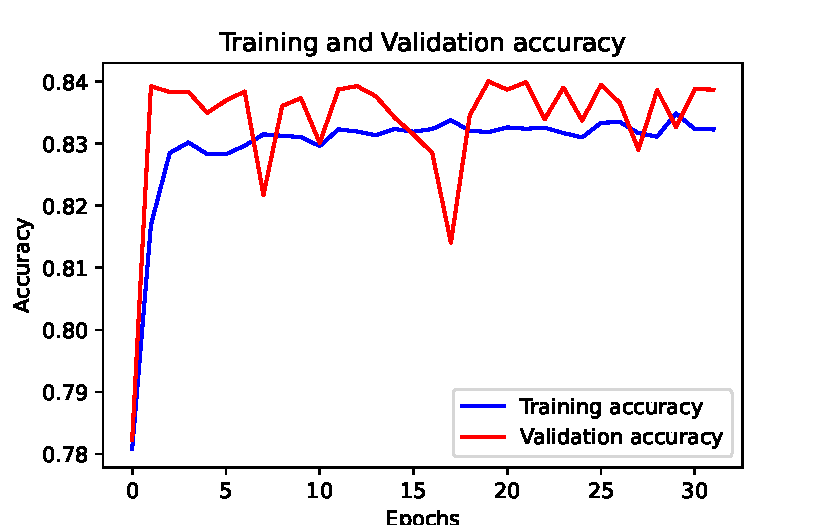
\includegraphics{RainAus_EDA_files/figure-pdf/unnamed-chunk-30-1.pdf}

}

\end{figure}

\begin{Shaded}
\begin{Highlighting}[]
\CommentTok{\# Predicting the test set results}
\NormalTok{y\_pred }\OperatorTok{=}\NormalTok{ model.predict(X\_test)}
\end{Highlighting}
\end{Shaded}

\begin{verbatim}

  1/910 ━━━━━━━━━━━━━━━━━━━━ 1:08 75ms/step
 74/910 ━━━━━━━━━━━━━━━━━━━━ 0s 691us/step 
149/910 ━━━━━━━━━━━━━━━━━━━━ 0s 684us/step
225/910 ━━━━━━━━━━━━━━━━━━━━ 0s 676us/step
296/910 ━━━━━━━━━━━━━━━━━━━━ 0s 684us/step
370/910 ━━━━━━━━━━━━━━━━━━━━ 0s 684us/step
443/910 ━━━━━━━━━━━━━━━━━━━━ 0s 686us/step
510/910 ━━━━━━━━━━━━━━━━━━━━ 0s 695us/step
577/910 ━━━━━━━━━━━━━━━━━━━━ 0s 702us/step
644/910 ━━━━━━━━━━━━━━━━━━━━ 0s 707us/step
710/910 ━━━━━━━━━━━━━━━━━━━━ 0s 712us/step
778/910 ━━━━━━━━━━━━━━━━━━━━ 0s 714us/step
846/910 ━━━━━━━━━━━━━━━━━━━━ 0s 717us/step
910/910 ━━━━━━━━━━━━━━━━━━━━ 0s 777us/step
910/910 ━━━━━━━━━━━━━━━━━━━━ 1s 777us/step
\end{verbatim}

\begin{Shaded}
\begin{Highlighting}[]
\NormalTok{y\_pred }\OperatorTok{=}\NormalTok{ (y\_pred }\OperatorTok{\textgreater{}} \FloatTok{0.5}\NormalTok{)}

\BuiltInTok{print}\NormalTok{(classification\_report(y\_test, y\_pred))}
\end{Highlighting}
\end{Shaded}

\begin{verbatim}
              precision    recall  f1-score   support

           0       0.86      0.94      0.90     22672
           1       0.70      0.47      0.56      6420

    accuracy                           0.84     29092
   macro avg       0.78      0.71      0.73     29092
weighted avg       0.83      0.84      0.83     29092
\end{verbatim}

\begin{center}\rule{0.5\linewidth}{0.5pt}\end{center}

\hypertarget{catboost}{%
\subsubsection{CatBoost}\label{catboost}}

\begin{itemize}
\item
  Catboost is a machine learning algorithm that excels in classification
  and regression tasks. As a \textbf{gradient boosting} algorithm, it
  builds an ensemble of decision trees, where each tree corrects the
  errors of the previous ones. This iterative process enhances the
  model's accuracy and robustness.
\item
  \textbf{FUNCTIONING}

  Catboost follows the principles of gradient boosting but introduces
  several unique innovations:

  \begin{itemize}
  \item
    \emph{Initialization:} The algorithm begins with a simple initial
    model, such as predicting the \textbf{mean value} for regression or
    \textbf{uniform probability} for classification.
  \item
    \emph{Sequential Tree Building:} Decision trees are constructed one
    by one. Each tree is designed to minimize a specified loss function
    by addressing the errors from previous trees.
  \item
    \emph{Model Update:} Newly built tree is added to the model,
    refining it.
  \item
    \emph{Iteration:} The process repeats until the stopping criterion
    is met.
  \end{itemize}
\item
  \textbf{Key Concepts:}

  \begin{itemize}
  \item
    \ul{Gradient Boosting:} Ensemble learning technique that combines
    weak prediction models, typically prediction trees, to form a strong
    predictive model. It iteratively adds new models to the ensemble.
  \item
    \ul{Handling Categorical Features:} It handles categorical features
    directly, without requiring extensive preprocessing. Very effective
    for real-world datasets that contain qualitative data, improving the
    performance.
  \item
    Learning Rate: The learning rate in CatBoost controls the step size
    at which the model learns during boosting. CatBoost automatically
    selects an optimal learning rate based on the dataset's features,
    striking a \textbf{balance} between \textbf{learning speed} and
    \textbf{model accuracy.} This helps achieving better performance
    with minimal tuning.
  \end{itemize}

  \begin{figure}

  {\centering 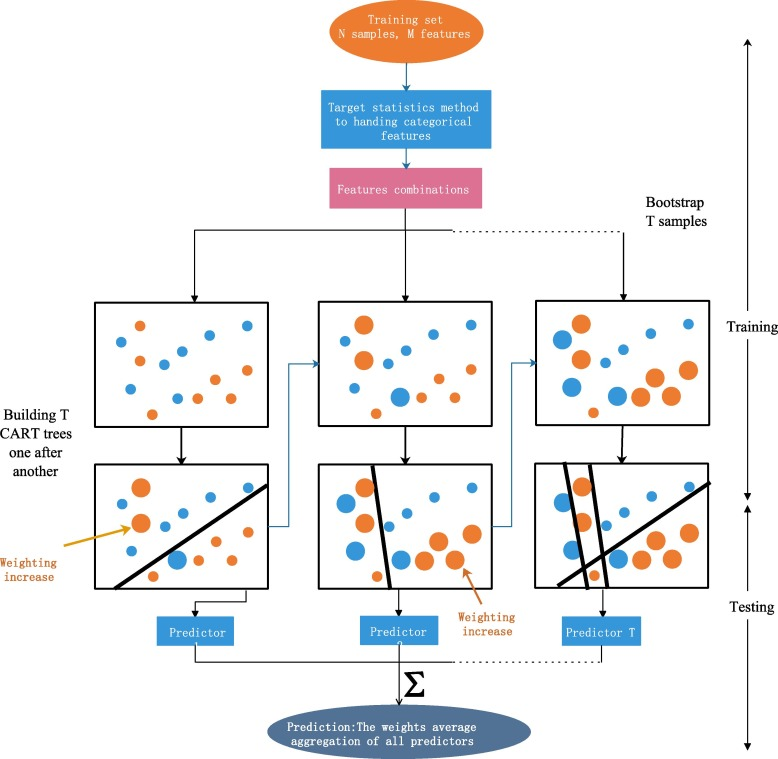
\includegraphics{CaBoostPicture.jpg}

  }

  \caption{Sequential Tree Building approach}

  \end{figure}
\end{itemize}

\begin{center}\rule{0.5\linewidth}{0.5pt}\end{center}

\begin{Shaded}
\begin{Highlighting}[]
\CommentTok{\# Load data}
\NormalTok{data }\OperatorTok{=}\NormalTok{ pd.read\_csv(}\StringTok{"weatherAUS.csv"}\NormalTok{)}

\CommentTok{\# Define columns with missing values}
\NormalTok{numeric\_features }\OperatorTok{=}\NormalTok{ data.select\_dtypes(include}\OperatorTok{=}\NormalTok{[}\StringTok{\textquotesingle{}float64\textquotesingle{}}\NormalTok{, }\StringTok{\textquotesingle{}int64\textquotesingle{}}\NormalTok{]).columns}
\NormalTok{categorical\_features }\OperatorTok{=}\NormalTok{ data.select\_dtypes(include}\OperatorTok{=}\NormalTok{[}\StringTok{\textquotesingle{}object\textquotesingle{}}\NormalTok{]).columns}

\CommentTok{\# Fill missing values}
\ControlFlowTok{for}\NormalTok{ col }\KeywordTok{in}\NormalTok{ numeric\_features:}
\NormalTok{    data[col] }\OperatorTok{=}\NormalTok{ data[col].fillna(data[col].median())}

\ControlFlowTok{for}\NormalTok{ col }\KeywordTok{in}\NormalTok{ categorical\_features:}
\NormalTok{    data[col] }\OperatorTok{=}\NormalTok{ data[col].fillna(data[col].mode()[}\DecValTok{0}\NormalTok{])}

\CommentTok{\# Prepare features and labels}
\NormalTok{X }\OperatorTok{=}\NormalTok{ data.drop(columns}\OperatorTok{=}\NormalTok{[}\StringTok{\textquotesingle{}RainTomorrow\textquotesingle{}}\NormalTok{])}
\NormalTok{y }\OperatorTok{=}\NormalTok{ data[}\StringTok{\textquotesingle{}RainTomorrow\textquotesingle{}}\NormalTok{]}

\CommentTok{\# Ensure that \textquotesingle{}RainTomorrow\textquotesingle{} is not included in categorical\_features}
\NormalTok{categorical\_features }\OperatorTok{=}\NormalTok{ [col }\ControlFlowTok{for}\NormalTok{ col }\KeywordTok{in}\NormalTok{ categorical\_features }\ControlFlowTok{if}\NormalTok{ col }\OperatorTok{!=} \StringTok{\textquotesingle{}RainTomorrow\textquotesingle{}}\NormalTok{]}

\CommentTok{\# Split the data}
\NormalTok{X\_train, X\_test, y\_train, y\_test }\OperatorTok{=}\NormalTok{ train\_test\_split(X, y, test\_size}\OperatorTok{=}\FloatTok{0.2}\NormalTok{, random\_state}\OperatorTok{=}\DecValTok{42}\NormalTok{)}

\CommentTok{\# Create CatBoost Pool}
\NormalTok{train\_pool }\OperatorTok{=}\NormalTok{ Pool(data}\OperatorTok{=}\NormalTok{X\_train, label}\OperatorTok{=}\NormalTok{y\_train, cat\_features}\OperatorTok{=}\NormalTok{categorical\_features)}
\NormalTok{test\_pool }\OperatorTok{=}\NormalTok{ Pool(data}\OperatorTok{=}\NormalTok{X\_test, label}\OperatorTok{=}\NormalTok{y\_test, cat\_features}\OperatorTok{=}\NormalTok{categorical\_features)}

\CommentTok{\# Initialize CatBoost model}
\NormalTok{model }\OperatorTok{=}\NormalTok{ CatBoostClassifier(iterations}\OperatorTok{=}\DecValTok{100}\NormalTok{, depth}\OperatorTok{=}\DecValTok{6}\NormalTok{, learning\_rate}\OperatorTok{=}\FloatTok{0.1}\NormalTok{, loss\_function}\OperatorTok{=}\StringTok{\textquotesingle{}Logloss\textquotesingle{}}\NormalTok{, verbose}\OperatorTok{=}\VariableTok{True}\NormalTok{)}

\CommentTok{\# Train the model}
\NormalTok{model.fit(train\_pool)}
\end{Highlighting}
\end{Shaded}

\begin{verbatim}
0:  learn: 0.6270827    total: 219ms    remaining: 21.7s
1:  learn: 0.5717355    total: 286ms    remaining: 14s
2:  learn: 0.5288813    total: 353ms    remaining: 11.4s
3:  learn: 0.4973616    total: 431ms    remaining: 10.3s
4:  learn: 0.4714247    total: 500ms    remaining: 9.5s
5:  learn: 0.4506941    total: 575ms    remaining: 9.01s
6:  learn: 0.4342015    total: 643ms    remaining: 8.54s
7:  learn: 0.4215802    total: 710ms    remaining: 8.17s
8:  learn: 0.4108237    total: 791ms    remaining: 8s
9:  learn: 0.4027844    total: 863ms    remaining: 7.77s
10: learn: 0.3964012    total: 922ms    remaining: 7.46s
11: learn: 0.3904812    total: 978ms    remaining: 7.17s
12: learn: 0.3857214    total: 1.03s    remaining: 6.89s
13: learn: 0.3821417    total: 1.09s    remaining: 6.68s
14: learn: 0.3791560    total: 1.14s    remaining: 6.48s
15: learn: 0.3756302    total: 1.2s remaining: 6.28s
16: learn: 0.3729289    total: 1.25s    remaining: 6.11s
17: learn: 0.3708955    total: 1.3s remaining: 5.94s
18: learn: 0.3682472    total: 1.36s    remaining: 5.79s
19: learn: 0.3661856    total: 1.41s    remaining: 5.63s
20: learn: 0.3643729    total: 1.46s    remaining: 5.48s
21: learn: 0.3627445    total: 1.51s    remaining: 5.36s
22: learn: 0.3612535    total: 1.56s    remaining: 5.23s
23: learn: 0.3600752    total: 1.61s    remaining: 5.11s
24: learn: 0.3588005    total: 1.67s    remaining: 5s
25: learn: 0.3577698    total: 1.72s    remaining: 4.88s
26: learn: 0.3565534    total: 1.77s    remaining: 4.78s
27: learn: 0.3557328    total: 1.81s    remaining: 4.67s
28: learn: 0.3549938    total: 1.86s    remaining: 4.57s
29: learn: 0.3542297    total: 1.93s    remaining: 4.5s
30: learn: 0.3535394    total: 1.98s    remaining: 4.41s
31: learn: 0.3529597    total: 2.03s    remaining: 4.32s
32: learn: 0.3523279    total: 2.08s    remaining: 4.22s
33: learn: 0.3517458    total: 2.13s    remaining: 4.14s
34: learn: 0.3512072    total: 2.19s    remaining: 4.06s
35: learn: 0.3508272    total: 2.24s    remaining: 3.98s
36: learn: 0.3503401    total: 2.29s    remaining: 3.9s
37: learn: 0.3499323    total: 2.34s    remaining: 3.83s
38: learn: 0.3492855    total: 2.4s remaining: 3.75s
39: learn: 0.3487488    total: 2.45s    remaining: 3.68s
40: learn: 0.3483432    total: 2.51s    remaining: 3.61s
41: learn: 0.3477834    total: 2.56s    remaining: 3.53s
42: learn: 0.3473898    total: 2.61s    remaining: 3.46s
43: learn: 0.3469520    total: 2.66s    remaining: 3.39s
44: learn: 0.3465444    total: 2.71s    remaining: 3.31s
45: learn: 0.3462299    total: 2.76s    remaining: 3.24s
46: learn: 0.3459126    total: 2.82s    remaining: 3.18s
47: learn: 0.3456854    total: 2.87s    remaining: 3.11s
48: learn: 0.3454154    total: 2.92s    remaining: 3.04s
49: learn: 0.3450373    total: 2.97s    remaining: 2.97s
50: learn: 0.3447874    total: 3.03s    remaining: 2.91s
51: learn: 0.3445977    total: 3.08s    remaining: 2.84s
52: learn: 0.3442821    total: 3.13s    remaining: 2.78s
53: learn: 0.3440186    total: 3.18s    remaining: 2.71s
54: learn: 0.3436322    total: 3.23s    remaining: 2.65s
55: learn: 0.3433082    total: 3.31s    remaining: 2.6s
56: learn: 0.3430198    total: 3.37s    remaining: 2.54s
57: learn: 0.3427467    total: 3.43s    remaining: 2.49s
58: learn: 0.3424777    total: 3.49s    remaining: 2.43s
59: learn: 0.3422668    total: 3.55s    remaining: 2.37s
60: learn: 0.3420107    total: 3.61s    remaining: 2.31s
61: learn: 0.3417488    total: 3.66s    remaining: 2.24s
62: learn: 0.3415566    total: 3.71s    remaining: 2.18s
63: learn: 0.3412778    total: 3.78s    remaining: 2.12s
64: learn: 0.3409374    total: 3.85s    remaining: 2.07s
65: learn: 0.3407438    total: 3.91s    remaining: 2.02s
66: learn: 0.3405608    total: 3.98s    remaining: 1.96s
67: learn: 0.3403057    total: 4.04s    remaining: 1.9s
68: learn: 0.3401749    total: 4.1s remaining: 1.84s
69: learn: 0.3400269    total: 4.17s    remaining: 1.79s
70: learn: 0.3398812    total: 4.23s    remaining: 1.73s
71: learn: 0.3396056    total: 4.3s remaining: 1.67s
72: learn: 0.3393633    total: 4.37s    remaining: 1.62s
73: learn: 0.3391712    total: 4.44s    remaining: 1.56s
74: learn: 0.3389652    total: 4.5s remaining: 1.5s
75: learn: 0.3388147    total: 4.57s    remaining: 1.44s
76: learn: 0.3386354    total: 4.63s    remaining: 1.38s
77: learn: 0.3384554    total: 4.76s    remaining: 1.34s
78: learn: 0.3381688    total: 4.85s    remaining: 1.29s
79: learn: 0.3379327    total: 4.9s remaining: 1.23s
80: learn: 0.3376758    total: 4.96s    remaining: 1.16s
81: learn: 0.3374471    total: 5.01s    remaining: 1.1s
82: learn: 0.3371651    total: 5.06s    remaining: 1.03s
83: learn: 0.3369951    total: 5.11s    remaining: 973ms
84: learn: 0.3368574    total: 5.16s    remaining: 911ms
85: learn: 0.3367000    total: 5.21s    remaining: 849ms
86: learn: 0.3365668    total: 5.26s    remaining: 787ms
87: learn: 0.3364186    total: 5.32s    remaining: 726ms
88: learn: 0.3362673    total: 5.38s    remaining: 665ms
89: learn: 0.3361320    total: 5.44s    remaining: 605ms
90: learn: 0.3358321    total: 5.5s remaining: 544ms
91: learn: 0.3357172    total: 5.56s    remaining: 484ms
92: learn: 0.3355988    total: 5.62s    remaining: 423ms
93: learn: 0.3354584    total: 5.71s    remaining: 365ms
94: learn: 0.3352782    total: 5.8s remaining: 305ms
95: learn: 0.3350775    total: 5.86s    remaining: 244ms
96: learn: 0.3349315    total: 5.92s    remaining: 183ms
97: learn: 0.3346553    total: 5.97s    remaining: 122ms
98: learn: 0.3345161    total: 6.03s    remaining: 60.9ms
99: learn: 0.3343546    total: 6.08s    remaining: 0us
<catboost.core.CatBoostClassifier object at 0x000001EBEA834EF0>
\end{verbatim}

\begin{Shaded}
\begin{Highlighting}[]
\CommentTok{\# Get evaluation results}
\NormalTok{evals\_result }\OperatorTok{=}\NormalTok{ model.get\_evals\_result()}

\CommentTok{\# Print the loss at each iteration}
\NormalTok{losses }\OperatorTok{=}\NormalTok{ evals\_result[}\StringTok{\textquotesingle{}learn\textquotesingle{}}\NormalTok{][}\StringTok{\textquotesingle{}Logloss\textquotesingle{}}\NormalTok{]}
\ControlFlowTok{for}\NormalTok{ i, loss }\KeywordTok{in} \BuiltInTok{enumerate}\NormalTok{(losses):}
    \BuiltInTok{print}\NormalTok{(}\SpecialStringTok{f\textquotesingle{}Iteration }\SpecialCharTok{\{}\NormalTok{i}\SpecialCharTok{\}}\SpecialStringTok{: Loss = }\SpecialCharTok{\{}\NormalTok{loss}\SpecialCharTok{\}}\SpecialStringTok{\textquotesingle{}}\NormalTok{)}
\end{Highlighting}
\end{Shaded}

\begin{verbatim}
Iteration 0: Loss = 0.6270827237767883
Iteration 1: Loss = 0.5717354793926579
Iteration 2: Loss = 0.5288812628855518
Iteration 3: Loss = 0.4973616233888124
Iteration 4: Loss = 0.4714247258482001
Iteration 5: Loss = 0.4506941309414565
Iteration 6: Loss = 0.4342015017759755
Iteration 7: Loss = 0.42158016843606083
Iteration 8: Loss = 0.4108236964050978
Iteration 9: Loss = 0.4027843769336262
Iteration 10: Loss = 0.3964011539734376
Iteration 11: Loss = 0.3904811695456526
Iteration 12: Loss = 0.3857213945284449
Iteration 13: Loss = 0.38214174768108533
Iteration 14: Loss = 0.37915597470494844
Iteration 15: Loss = 0.3756302421858873
Iteration 16: Loss = 0.3729288881969476
Iteration 17: Loss = 0.37089550581782865
Iteration 18: Loss = 0.3682472406955625
Iteration 19: Loss = 0.36618560966383606
Iteration 20: Loss = 0.36437285404104275
Iteration 21: Loss = 0.36274449459763336
Iteration 22: Loss = 0.3612535036541703
Iteration 23: Loss = 0.36007523330820534
Iteration 24: Loss = 0.3588005188854733
Iteration 25: Loss = 0.35776978436870616
Iteration 26: Loss = 0.3565534161036887
Iteration 27: Loss = 0.3557328195813623
Iteration 28: Loss = 0.3549938433377035
Iteration 29: Loss = 0.354229739887142
Iteration 30: Loss = 0.3535394131996704
Iteration 31: Loss = 0.35295974960899706
Iteration 32: Loss = 0.3523278904852756
Iteration 33: Loss = 0.35174578694864356
Iteration 34: Loss = 0.3512072485769523
Iteration 35: Loss = 0.3508271928376375
Iteration 36: Loss = 0.3503401363739203
Iteration 37: Loss = 0.3499322739748575
Iteration 38: Loss = 0.34928546614639683
Iteration 39: Loss = 0.3487487752654309
Iteration 40: Loss = 0.34834318752385574
Iteration 41: Loss = 0.3477833751071816
Iteration 42: Loss = 0.34738981047673967
Iteration 43: Loss = 0.34695195123232153
Iteration 44: Loss = 0.3465443798518192
Iteration 45: Loss = 0.3462298504372243
Iteration 46: Loss = 0.3459125687418106
Iteration 47: Loss = 0.3456854191770339
Iteration 48: Loss = 0.3454153942598656
Iteration 49: Loss = 0.3450373194250657
Iteration 50: Loss = 0.34478744037696357
Iteration 51: Loss = 0.3445977362087669
Iteration 52: Loss = 0.34428206455429383
Iteration 53: Loss = 0.3440186374520361
Iteration 54: Loss = 0.3436321515239965
Iteration 55: Loss = 0.3433081702001865
Iteration 56: Loss = 0.34301976783293137
Iteration 57: Loss = 0.342746698825511
Iteration 58: Loss = 0.34247771072910294
Iteration 59: Loss = 0.3422668333935659
Iteration 60: Loss = 0.3420107164587027
Iteration 61: Loss = 0.3417488039926738
Iteration 62: Loss = 0.34155661377551305
Iteration 63: Loss = 0.34127779034283395
Iteration 64: Loss = 0.34093736745608966
Iteration 65: Loss = 0.34074379035181296
Iteration 66: Loss = 0.34056082432755497
Iteration 67: Loss = 0.34030574760411686
Iteration 68: Loss = 0.34017494503364315
Iteration 69: Loss = 0.3400269046890985
Iteration 70: Loss = 0.33988116675069346
Iteration 71: Loss = 0.3396056351189006
Iteration 72: Loss = 0.33936332873521713
Iteration 73: Loss = 0.33917120390971744
Iteration 74: Loss = 0.3389652301662063
Iteration 75: Loss = 0.33881472134385904
Iteration 76: Loss = 0.33863537705401003
Iteration 77: Loss = 0.3384554262179324
Iteration 78: Loss = 0.33816879583522697
Iteration 79: Loss = 0.33793270188907587
Iteration 80: Loss = 0.3376758355898742
Iteration 81: Loss = 0.33744705126759483
Iteration 82: Loss = 0.33716505776956657
Iteration 83: Loss = 0.33699505027251486
Iteration 84: Loss = 0.3368573956806205
Iteration 85: Loss = 0.33669996281432946
Iteration 86: Loss = 0.3365667917803073
Iteration 87: Loss = 0.33641864645578584
Iteration 88: Loss = 0.33626733591787766
Iteration 89: Loss = 0.33613197490343427
Iteration 90: Loss = 0.33583206856058956
Iteration 91: Loss = 0.33571723342677906
Iteration 92: Loss = 0.3355988366380124
Iteration 93: Loss = 0.3354584312006883
Iteration 94: Loss = 0.33527819696879657
Iteration 95: Loss = 0.33507752803669977
Iteration 96: Loss = 0.3349315124033232
Iteration 97: Loss = 0.3346552828256837
Iteration 98: Loss = 0.3345161257026082
Iteration 99: Loss = 0.33435455914758744
\end{verbatim}

\begin{Shaded}
\begin{Highlighting}[]
\CommentTok{\# Make predictions}
\NormalTok{preds }\OperatorTok{=}\NormalTok{ model.predict(test\_pool)}

\CommentTok{\# Evaluate the model}
\NormalTok{accuracy }\OperatorTok{=}\NormalTok{ (preds }\OperatorTok{==}\NormalTok{ y\_test).mean()}
\BuiltInTok{print}\NormalTok{(}\SpecialStringTok{f\textquotesingle{}Accuracy: }\SpecialCharTok{\{}\NormalTok{accuracy}\SpecialCharTok{\}}\SpecialStringTok{\textquotesingle{}}\NormalTok{)}
\end{Highlighting}
\end{Shaded}

\begin{verbatim}
Accuracy: 0.8512649525642788
\end{verbatim}

\begin{Shaded}
\begin{Highlighting}[]
\BuiltInTok{print}\NormalTok{(classification\_report(y\_test, preds))}
\end{Highlighting}
\end{Shaded}

\begin{verbatim}
              precision    recall  f1-score   support

          No       0.87      0.95      0.91     22672
         Yes       0.74      0.50      0.60      6420

    accuracy                           0.85     29092
   macro avg       0.81      0.73      0.75     29092
weighted avg       0.84      0.85      0.84     29092
\end{verbatim}

\hypertarget{logistic-regression}{%
\subsubsection{Logistic Regression}\label{logistic-regression}}

\begin{itemize}
\item
  \textbf{Logistic Regression} is a supervised machine learning
  algorithm used for classification tasks where the goal is to predict
  the probability that an instance belongs to a given class or not. This
  model is used for binary classification where we use the sigmoid
  function, that takes input as independent variables and produces a
  probability value between 0 and 1.
\item
  \textbf{Key Concepts:}

  \begin{itemize}
  \item
    Logistic Regression predicts the output of a categorical dependent
    variable. In our case we have the target variable
    \emph{``RainTomorrow''} that has values ``yes'' and ``no''.
  \item
    It gives the probabilistic values which is between 0 and 1.
  \item
    Instead of fitting a regression line, we fit an \textbf{S shaped}
    logistic function, which predicts two maximum values.

    \begin{figure}

    {\centering 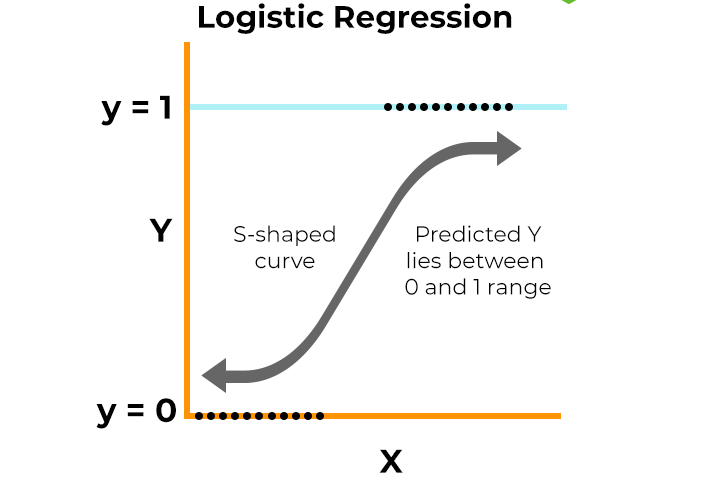
\includegraphics{LogRegPicture.png}

    }

    \caption{Sigmoid Function}

    \end{figure}
  \end{itemize}
\end{itemize}

\hfill\break

\begin{itemize}
\item
  {\textbf{Sigmoid function}} is a mathematical function used to map the
  predicted values to probabilities. It maps any real value into another
  value within the range of 0 and 1. This range is called the
  \textbf{Threshold value}.
\item
  \textbf{Types of Logistic regression}

  \begin{itemize}
  \item
    \ul{Binomial:} there can be only two possible types of dependent
    variables, such as 0 and 1, Pass or Fail, etc.
  \item
    \ul{Multinomial:} there can be 3 or more possible unordered types of
    the dependent variable, such as ``cat'', ``dogs'', or ``sheep''.
  \item
    \ul{Ordinal:} there can be 3 or more possible ordered types of
    dependent variables, such as ``low'', ``medium'', ``high''.
  \end{itemize}
\end{itemize}

\begin{Shaded}
\begin{Highlighting}[]
\NormalTok{data }\OperatorTok{=}\NormalTok{ pd.read\_csv(}\StringTok{"weatherAUS.csv"}\NormalTok{)}

\CommentTok{\# Define numerical and categorical columns}
\NormalTok{numerical\_cols }\OperatorTok{=}\NormalTok{ [}\StringTok{\textquotesingle{}MinTemp\textquotesingle{}}\NormalTok{, }\StringTok{\textquotesingle{}MaxTemp\textquotesingle{}}\NormalTok{, }\StringTok{\textquotesingle{}Rainfall\textquotesingle{}}\NormalTok{, }\StringTok{\textquotesingle{}Evaporation\textquotesingle{}}\NormalTok{, }\StringTok{\textquotesingle{}Sunshine\textquotesingle{}}\NormalTok{, }\StringTok{\textquotesingle{}WindGustSpeed\textquotesingle{}}\NormalTok{, }\StringTok{\textquotesingle{}WindSpeed9am\textquotesingle{}}\NormalTok{,}
                  \StringTok{\textquotesingle{}WindSpeed3pm\textquotesingle{}}\NormalTok{, }\StringTok{\textquotesingle{}Humidity9am\textquotesingle{}}\NormalTok{, }\StringTok{\textquotesingle{}Humidity3pm\textquotesingle{}}\NormalTok{, }\StringTok{\textquotesingle{}Pressure9am\textquotesingle{}}\NormalTok{, }\StringTok{\textquotesingle{}Pressure3pm\textquotesingle{}}\NormalTok{, }\StringTok{\textquotesingle{}Cloud9am\textquotesingle{}}\NormalTok{, }\StringTok{\textquotesingle{}Cloud3pm\textquotesingle{}}\NormalTok{,}
                  \StringTok{\textquotesingle{}Temp9am\textquotesingle{}}\NormalTok{, }\StringTok{\textquotesingle{}Temp3pm\textquotesingle{}}\NormalTok{]}
                  
\NormalTok{categorical\_cols }\OperatorTok{=}\NormalTok{ [}\StringTok{\textquotesingle{}WindGustDir\textquotesingle{}}\NormalTok{, }\StringTok{\textquotesingle{}WindDir9am\textquotesingle{}}\NormalTok{, }\StringTok{\textquotesingle{}WindDir3pm\textquotesingle{}}\NormalTok{, }\StringTok{\textquotesingle{}RainToday\textquotesingle{}}\NormalTok{]}


\CommentTok{\# Preprocessing for numerical data: Impute missing values with median and scale}
\NormalTok{numerical\_transformer }\OperatorTok{=}\NormalTok{ Pipeline(steps}\OperatorTok{=}\NormalTok{[}
\NormalTok{    (}\StringTok{\textquotesingle{}imputer\textquotesingle{}}\NormalTok{, SimpleImputer(strategy}\OperatorTok{=}\StringTok{\textquotesingle{}median\textquotesingle{}}\NormalTok{)),}
\NormalTok{    (}\StringTok{\textquotesingle{}scaler\textquotesingle{}}\NormalTok{, StandardScaler())}
\NormalTok{])}


\CommentTok{\# Preprocessing for categorical data: Impute missing values with mode and one{-}hot encode}
\NormalTok{categorical\_transformer }\OperatorTok{=}\NormalTok{ Pipeline(steps}\OperatorTok{=}\NormalTok{[}
\NormalTok{    (}\StringTok{\textquotesingle{}imputer\textquotesingle{}}\NormalTok{, SimpleImputer(strategy}\OperatorTok{=}\StringTok{\textquotesingle{}most\_frequent\textquotesingle{}}\NormalTok{)),}
\NormalTok{    (}\StringTok{\textquotesingle{}onehot\textquotesingle{}}\NormalTok{, OneHotEncoder(handle\_unknown}\OperatorTok{=}\StringTok{\textquotesingle{}ignore\textquotesingle{}}\NormalTok{))}
\NormalTok{])}


\CommentTok{\# Bundle preprocessing for numerical and categorical data}
\NormalTok{preprocessor }\OperatorTok{=}\NormalTok{ ColumnTransformer(}
\NormalTok{    transformers}\OperatorTok{=}\NormalTok{[}
\NormalTok{        (}\StringTok{\textquotesingle{}num\textquotesingle{}}\NormalTok{, numerical\_transformer, numerical\_cols),}
\NormalTok{        (}\StringTok{\textquotesingle{}cat\textquotesingle{}}\NormalTok{, categorical\_transformer, categorical\_cols)}
\NormalTok{    ])}

\CommentTok{\# Prepare the data}
\NormalTok{X }\OperatorTok{=}\NormalTok{ data.drop(columns}\OperatorTok{=}\NormalTok{[}\StringTok{\textquotesingle{}Date\textquotesingle{}}\NormalTok{, }\StringTok{\textquotesingle{}Location\textquotesingle{}}\NormalTok{, }\StringTok{\textquotesingle{}RainTomorrow\textquotesingle{}}\NormalTok{])}
\NormalTok{y }\OperatorTok{=}\NormalTok{ data[}\StringTok{\textquotesingle{}RainTomorrow\textquotesingle{}}\NormalTok{]}

\CommentTok{\# Apply label encoding to the target variable}
\NormalTok{label\_encoder }\OperatorTok{=}\NormalTok{ LabelEncoder()}
\NormalTok{y }\OperatorTok{=}\NormalTok{ label\_encoder.fit\_transform(y)}

\CommentTok{\# Split the data into training and testing sets}
\NormalTok{X\_train, X\_test, y\_train, y\_test }\OperatorTok{=}\NormalTok{ train\_test\_split(X, y, test\_size}\OperatorTok{=}\FloatTok{0.2}\NormalTok{, random\_state}\OperatorTok{=}\DecValTok{42}\NormalTok{)}

\CommentTok{\# Create and train the logistic regression model}
\NormalTok{model }\OperatorTok{=}\NormalTok{ Pipeline(steps}\OperatorTok{=}\NormalTok{[}
\NormalTok{    (}\StringTok{\textquotesingle{}preprocessor\textquotesingle{}}\NormalTok{, preprocessor),}
\NormalTok{    (}\StringTok{\textquotesingle{}classifier\textquotesingle{}}\NormalTok{, LogisticRegression(max\_iter}\OperatorTok{=}\DecValTok{1000}\NormalTok{))}
\NormalTok{])}

\NormalTok{model.fit(X\_train, y\_train)}
\end{Highlighting}
\end{Shaded}

\begin{verbatim}
Pipeline(steps=[('preprocessor',
                 ColumnTransformer(transformers=[('num',
                                                  Pipeline(steps=[('imputer',
                                                                   SimpleImputer(strategy='median')),
                                                                  ('scaler',
                                                                   StandardScaler())]),
                                                  ['MinTemp', 'MaxTemp',
                                                   'Rainfall', 'Evaporation',
                                                   'Sunshine', 'WindGustSpeed',
                                                   'WindSpeed9am',
                                                   'WindSpeed3pm',
                                                   'Humidity9am', 'Humidity3pm',
                                                   'Pressure9am', 'Pressure3pm',
                                                   'Cloud9am', 'Cloud3pm',
                                                   'Temp9am', 'Temp3pm']),
                                                 ('cat',
                                                  Pipeline(steps=[('imputer',
                                                                   SimpleImputer(strategy='most_frequent')),
                                                                  ('onehot',
                                                                   OneHotEncoder(handle_unknown='ignore'))]),
                                                  ['WindGustDir', 'WindDir9am',
                                                   'WindDir3pm',
                                                   'RainToday'])])),
                ('classifier', LogisticRegression(max_iter=1000))])
\end{verbatim}

\begin{Shaded}
\begin{Highlighting}[]
\CommentTok{\# Make predictions}
\NormalTok{y\_pred }\OperatorTok{=}\NormalTok{ model.predict(X\_test)}

\CommentTok{\# Evaluate the model}
\NormalTok{accuracy }\OperatorTok{=}\NormalTok{ accuracy\_score(y\_test, y\_pred)}
\NormalTok{conf\_matrix }\OperatorTok{=}\NormalTok{ confusion\_matrix(y\_test, y\_pred)}
\NormalTok{class\_report }\OperatorTok{=}\NormalTok{ classification\_report(y\_test, y\_pred, zero\_division}\OperatorTok{=}\DecValTok{0}\NormalTok{)}

\BuiltInTok{print}\NormalTok{(}\StringTok{"Accuracy:"}\NormalTok{, accuracy)}
\end{Highlighting}
\end{Shaded}

\begin{verbatim}
Accuracy: 0.8231472569778633
\end{verbatim}

\begin{Shaded}
\begin{Highlighting}[]
\BuiltInTok{print}\NormalTok{(}\StringTok{"Confusion Matrix:}\CharTok{\textbackslash{}n}\StringTok{"}\NormalTok{, conf\_matrix)}
\end{Highlighting}
\end{Shaded}

\begin{verbatim}
Confusion Matrix:
 [[20779  1233     0]
 [ 3252  3168     0]
 [  584    76     0]]
\end{verbatim}

\begin{Shaded}
\begin{Highlighting}[]
\BuiltInTok{print}\NormalTok{(}\StringTok{"Classification Report:}\CharTok{\textbackslash{}n}\StringTok{"}\NormalTok{, class\_report)}
\end{Highlighting}
\end{Shaded}

\begin{verbatim}
Classification Report:
               precision    recall  f1-score   support

           0       0.84      0.94      0.89     22012
           1       0.71      0.49      0.58      6420
           2       0.00      0.00      0.00       660

    accuracy                           0.82     29092
   macro avg       0.52      0.48      0.49     29092
weighted avg       0.79      0.82      0.80     29092
\end{verbatim}



\end{document}
